\documentclass{article}
\usepackage[utf8]{inputenc}
\usepackage{lmodern}
\usepackage{graphicx}
\usepackage{caption}
\usepackage{booktabs}
\usepackage[table]{xcolor}
\usepackage{hyperref}
\usepackage{rotating}
\usepackage[numbers]{natbib}
\usepackage{array} % For centering table columns
\usepackage{amsmath}
\usepackage{float}
\providecommand{\FloatBarrier}{}


\DeclareCaptionLabelFormat{boldfig}{\textbf{Fig #2}}
\captionsetup[figure]{labelformat=boldfig}

\graphicspath{ {./} }

\title{Open-Source News for Anticipatory Food Security Forecasting: Evidence from GDELT and FEWS NET}
\author{Marco Bertetti, Alvaro Calzadilla, Licia Capra, Lorenzo Lotti}
\begin{document}
\date{}

\maketitle

\begin{abstract}
Food insecurity affects millions globally, yet existing early warning systems depend on delayed or costly data sources. This study investigates whether open-source news text, processed at scale using NLP, can strengthen the anticipatory capacity of food security early-warning systems. Leveraging the GDELT Event and Global Knowledge Graph datasets, we extract conflict, aid, and food-related indicators from hundreds of thousands of news articles aligned with FEWS NET's IPC classifications across African countries. We develop a multi-task BERT-based pipeline to classify humanitarian text by impact type, urgency, and resource needs, complemented by domain-specific keyword extraction and sentiment scoring. A diagnostic comparison reveals that GDELT Events data tracks food security severity more reliably than the Global Knowledge Graph. In rolling temporal evaluations across 25 IPC assessment periods, GDELT-derived features with geographic context match lagged IPC scores for predicting food security levels (F1 0.834 vs.\ 0.836), with a small recent-period edge for GDELT-only over IPC-only (+0.020 F1 points in 2022--2024). Case studies across three crisis types confirm that news signals spike at or before IPC deterioration, including during assessment gaps. These findings suggest that streaming news data can serve as a scalable, near-real-time proxy for food security monitoring in data-scarce settings, illustrating how emerging open-data technologies can enhance anticipatory humanitarian action and inform forward-looking food security policy.
\end{abstract}


\section{Introduction}

Food security (FS) remains an elusive global goal. The United Nations Food and Agriculture Organisation (FAO)~\citep{FAO1996} defines it as a condition that \textit{``exists when all people, at all times, have physical and economic access to sufficient, safe and nutritious food to meet their dietary needs and food preferences for an active and healthy life''}. This definition rests on four key pillars: availability, access, utilisation, and stability, which together ensure that food is consistently obtainable and adequately used over time. Yet, despite decades of progress, chronic hunger and sudden-onset food crises are on the rise. FAO et al.~\citep{FAO2023} report that 702–828 million people were undernourished in 2021, and the World Food Programme (WFP) estimated that crisis-level or worse acute food insecurity threatened more than 282 million people in 2023~\citep{WFPhm2024}. Conflict, climate extremes, and economic shocks often interact, motivating the use of early-warning systems (EWS), such as FEWS NET and the Integrated Food Security Phase Classification (IPC), to anticipate humanitarian needs. However, these systems depend on household surveys, satellite images, or market data that are costly, irregular, or released with significant delay, highlighting the need for faster and more scalable predictors to support timely humanitarian response and resource allocation.\\

Despite growing interest in the use of large-scale media data for monitoring food security and humanitarian risk, there remains limited empirical understanding of what aspects of food insecurity such data can realistically capture. In particular, it is unclear how high-frequency news data varies in its spatial coverage, temporal responsiveness, and alignment with established food security indicators. This paper addresses this gap by providing a systematic, diagnostic comparison of the GDELT Events and Global Knowledge Graph datasets across African countries, evaluating their coverage patterns at multiple spatial scales and their empirical association with FEWS NET food security classifications. We focus on Africa, where food insecurity remains widespread and where both GDELT coverage and FEWS NET reporting are sufficiently dense to support systematic comparison. Specifically, this study asks whether and to what extent news-derived media signals can capture, at operational spatial and temporal scales, variation in acute food security conditions as measured by FEWS NET’s IPC classifications, how this capacity differs between GDELT's Event database and Global Knowledge Graph.

\paragraph{Contributions.}
This paper makes three contributions. First, it provides a systematic diagnostic comparison of GDELT Events and Global Knowledge Graph news representations for food security analysis, quantifying differences in spatial coverage, temporal responsiveness, and alignment with FEWS NET IPC classifications across African countries. Second, it introduces a scalable NLP pipeline that transforms news articles into interpretable, region--month humanitarian signals by combining structured event data, keyword-based indicators, and multi-task text classification. Third, it empirically characterises the structural limitations of media-derived signals, including spatial sparsity, reporting bias, and endogeneity, thereby delineating the conditions under which news-based features are informative for downstream food security modelling.\\

Unstructured text is an under-exploited but promising source of evidence for tracking food security, and a growing body of recent work has explored its potential in early warning and humanitarian analysis. Ba et al.~\citep{Ba2022} demonstrated this by processing news articles and YouTube transcripts related to Burkina Faso. After standard text pre-processing, the authors filtered and geolocated documents using a food-security lexicon and derived severity scores from crisis-related terms. Their findings, though spatially coarse and confined to a single country, showed that text can capture temporal and spatial variation with a single, automatically gathered data stream. \\

Fraiberger et al.~\citep{Fraiberger2023} scaled this approach by mining 11 million news articles from food-insecure countries between 1980 and 2020. Using 170 risk-related keywords (e.g., conflict, drought, agricultural pests), they improved IPC forecasts up to 12 months ahead, reducing prediction error by more than 40\%. Media signals also tended to lead traditional indicators; for example, reporting on a 2016 Fall Armyworm outbreak in South Sudan peaked several months before the corresponding IPC deterioration, while satellite NDVI declined only shortly beforehand. \\

Ahn et al.~\citep{Ahn2023} advanced this concept with \textit{HungerGist}, a multi-task transformer model trained on 53{,}000 articles from nine African countries. Relying solely on news text, it outperformed a baseline of expert indicators in predicting food insecurity, staple-price shocks, and social unrest. The model also produced interpretable “gists” that highlighted the phrases driving each forecast.\\

Recent synthesis work has begun to formalise the role of NLP within food security policymaking. Meeske et al.~\citep{Meeske2025} provide a comprehensive scoping review of NLP applications for food security, identifying early warning systems, crisis monitoring, and data-gap filling as core application areas. However, their review also highlights that most NLP-based food security studies remain at low technology-readiness levels, are rarely deployed operationally, and often lack rigorous validation against established food security benchmarks such as IPC classifications. Crucially, the review notes a disconnect between methodological innovation and policy-aligned evaluation, underscoring the need for diagnostic studies that explicitly assess what dimensions of food insecurity different NLP signals can and cannot capture.\\

Operational agencies are embedding similar tools. FAO's Data Lab~\citep{FAODataLab2024} scrapes web reports to update a food-loss database and track food-security sentiment. WFP's \textit{HungerMap Live}~\citep{WFPhm2024} merges text streams with other inputs and pilots an AI now-casting model projecting hunger 60 days ahead. Molenaar et al.~\citep{Molenaar2024} analysed around 38{,}000 food-related tweets; sentiment analysis and topic modelling produced themes mapping neatly onto FAO’s four FS pillars. Changes in topic prevalence and tone mirrored real-world conditions, though the authors note the need for broader social-media coverage and richer domain lexicons. Together, these studies show that textual data, from curated news to crowd-sourced posts, can complement or even supersede traditional indicators, though challenges remain in multilingual processing, finer spatial granularity, and rigorous validation.\\

Explainability and spatial bias have emerged as central concerns in text-based food security indicators. Valentin et al.~\citep{Valentin2024} propose a food-security indicator derived solely from news text at the subnational level, explicitly accounting for uneven media coverage and distinguishing between different crisis triggers. While their approach demonstrates the explanatory value of textual data and highlights the importance of correcting for reporting bias, it remains geographically confined and does not directly benchmark media-derived indicators against operational IPC classifications. This limits its ability to assess whether text-based signals align with the spatial and temporal decision scales used by humanitarian agencies.\\

Most recently, attention has shifted toward large language models (LLMs), whose rapidly expanding role across disaster-management tasks is now the subject of dedicated surveys~\citep{Lei2025}. Early evaluations probe both their capacity to forecast violent conflict from parametric knowledge and retrieval-augmented news context~\citep{Nemkova2025} and their ability to autonomously generate evidence-grounded humanitarian situation reports~\citep{Decostanzi2025}. These efforts highlight the promise of generative models for anticipatory monitoring, but also their current reliability limits in high-stakes settings, reinforcing the need for the kind of diagnostic, benchmark-grounded evaluation against operational IPC classifications that we pursue here.\\


\subsection{NLP in Related Domains}

While NLP for food security is emerging, related applications in disaster response, drought monitoring, conflict early warning, and climate-risk forecasting are more mature. Sodoge et al.~\citep{Sodoge2023} trained classifiers on German newspaper archives to detect drought impacts over time and across sectors (e.g., livestock, forestry), attaining 92–96 \% accuracy against independent assessment services. Sufi~\citep{Sufi2022} built an end-to-end disaster-detection platform using Twitter: bursts of negative posts were automatically labelled, clustered, and geolocated with high precision and recall. \\

Bridging formal and informal sources, Algiriyage et al.~\citep{Algiriyage2023} fused news articles and tweets during the 2015 Nepal earthquake, extracting “what–when–where” information. The integrated model outperformed social media alone, though scalability beyond that case remains to be proven. Reviews by Tounsi and Temimi~\citep{ExtremeWeatherReview2023} also highlight NLP's promise for extreme-weather detection, especially when combining media and social signals. \\

In conflict analytics, event databases such as ACLED and GDELT~\citep{GDELT2022} have long tracked unrest through media-reported incidents. Clustering these events helps forecast broader instability before it becomes visible through official channels. Common methods across these studies include topic modelling, sentiment analysis, and embeddings with interpretability layers.

These examples show how heterogeneous textual streams can enrich early-warning systems, automate expert reporting, and reduce bias, strengthening the case for adapting similar pipelines to food security.\\

Building on this foundation, our study examines whether continuously harvested news can serve as an operational input for food security analysis. We use NLP models to distil structured signals from GDELT’s Event and Global Knowledge Graph streams, extracting information related to conflict dynamics, humanitarian activity, and food-system stress. Additionally, we employ a multi-task BERT architecture to classify article content along dimensions such as impact type, urgency, and resource needs, and use these predictions as intermediate features in downstream food-security modelling. This design treats NLP not as a standalone forecasting tool, but as a mechanism for transforming unstructured text into interpretable signals that can be aligned with FEWS NET’s geolocated IPC classifications and integrated with conventional indicators.



\section{Methods}
\subsection{Data}

\subsubsection{FEWS NET Food Security Data}\label{sec:fewsnet_data}

The Famine Early Warning Systems Network (FEWS NET) is a leading source of sub-national food security data, originally established by USAID in 1985 in the wake of severe famines in Africa (notably the 1984–85 Ethiopian famine) \citep{spitzer2025respected}. Its mission has been to provide early warning of acute food insecurity to inform timely humanitarian response \citep{knibbs2025usaid}. FEWS NET works with international partners (e.g., NASA, NOAA, USDA) to integrate diverse inputs—satellite imagery, climate records, market prices, conflict events—into its analysis \citep{fewsnet2023ipc}. These are synthesized into regular, evidence-based forecasts published multiple times per year. Among these, the \textit{Food Security Outlook} reports are a cornerstone product, providing early warnings of hunger crises with 4–6 month lead times~\citep{backer2021validating}.

\begin{figure}[ht]
\centering
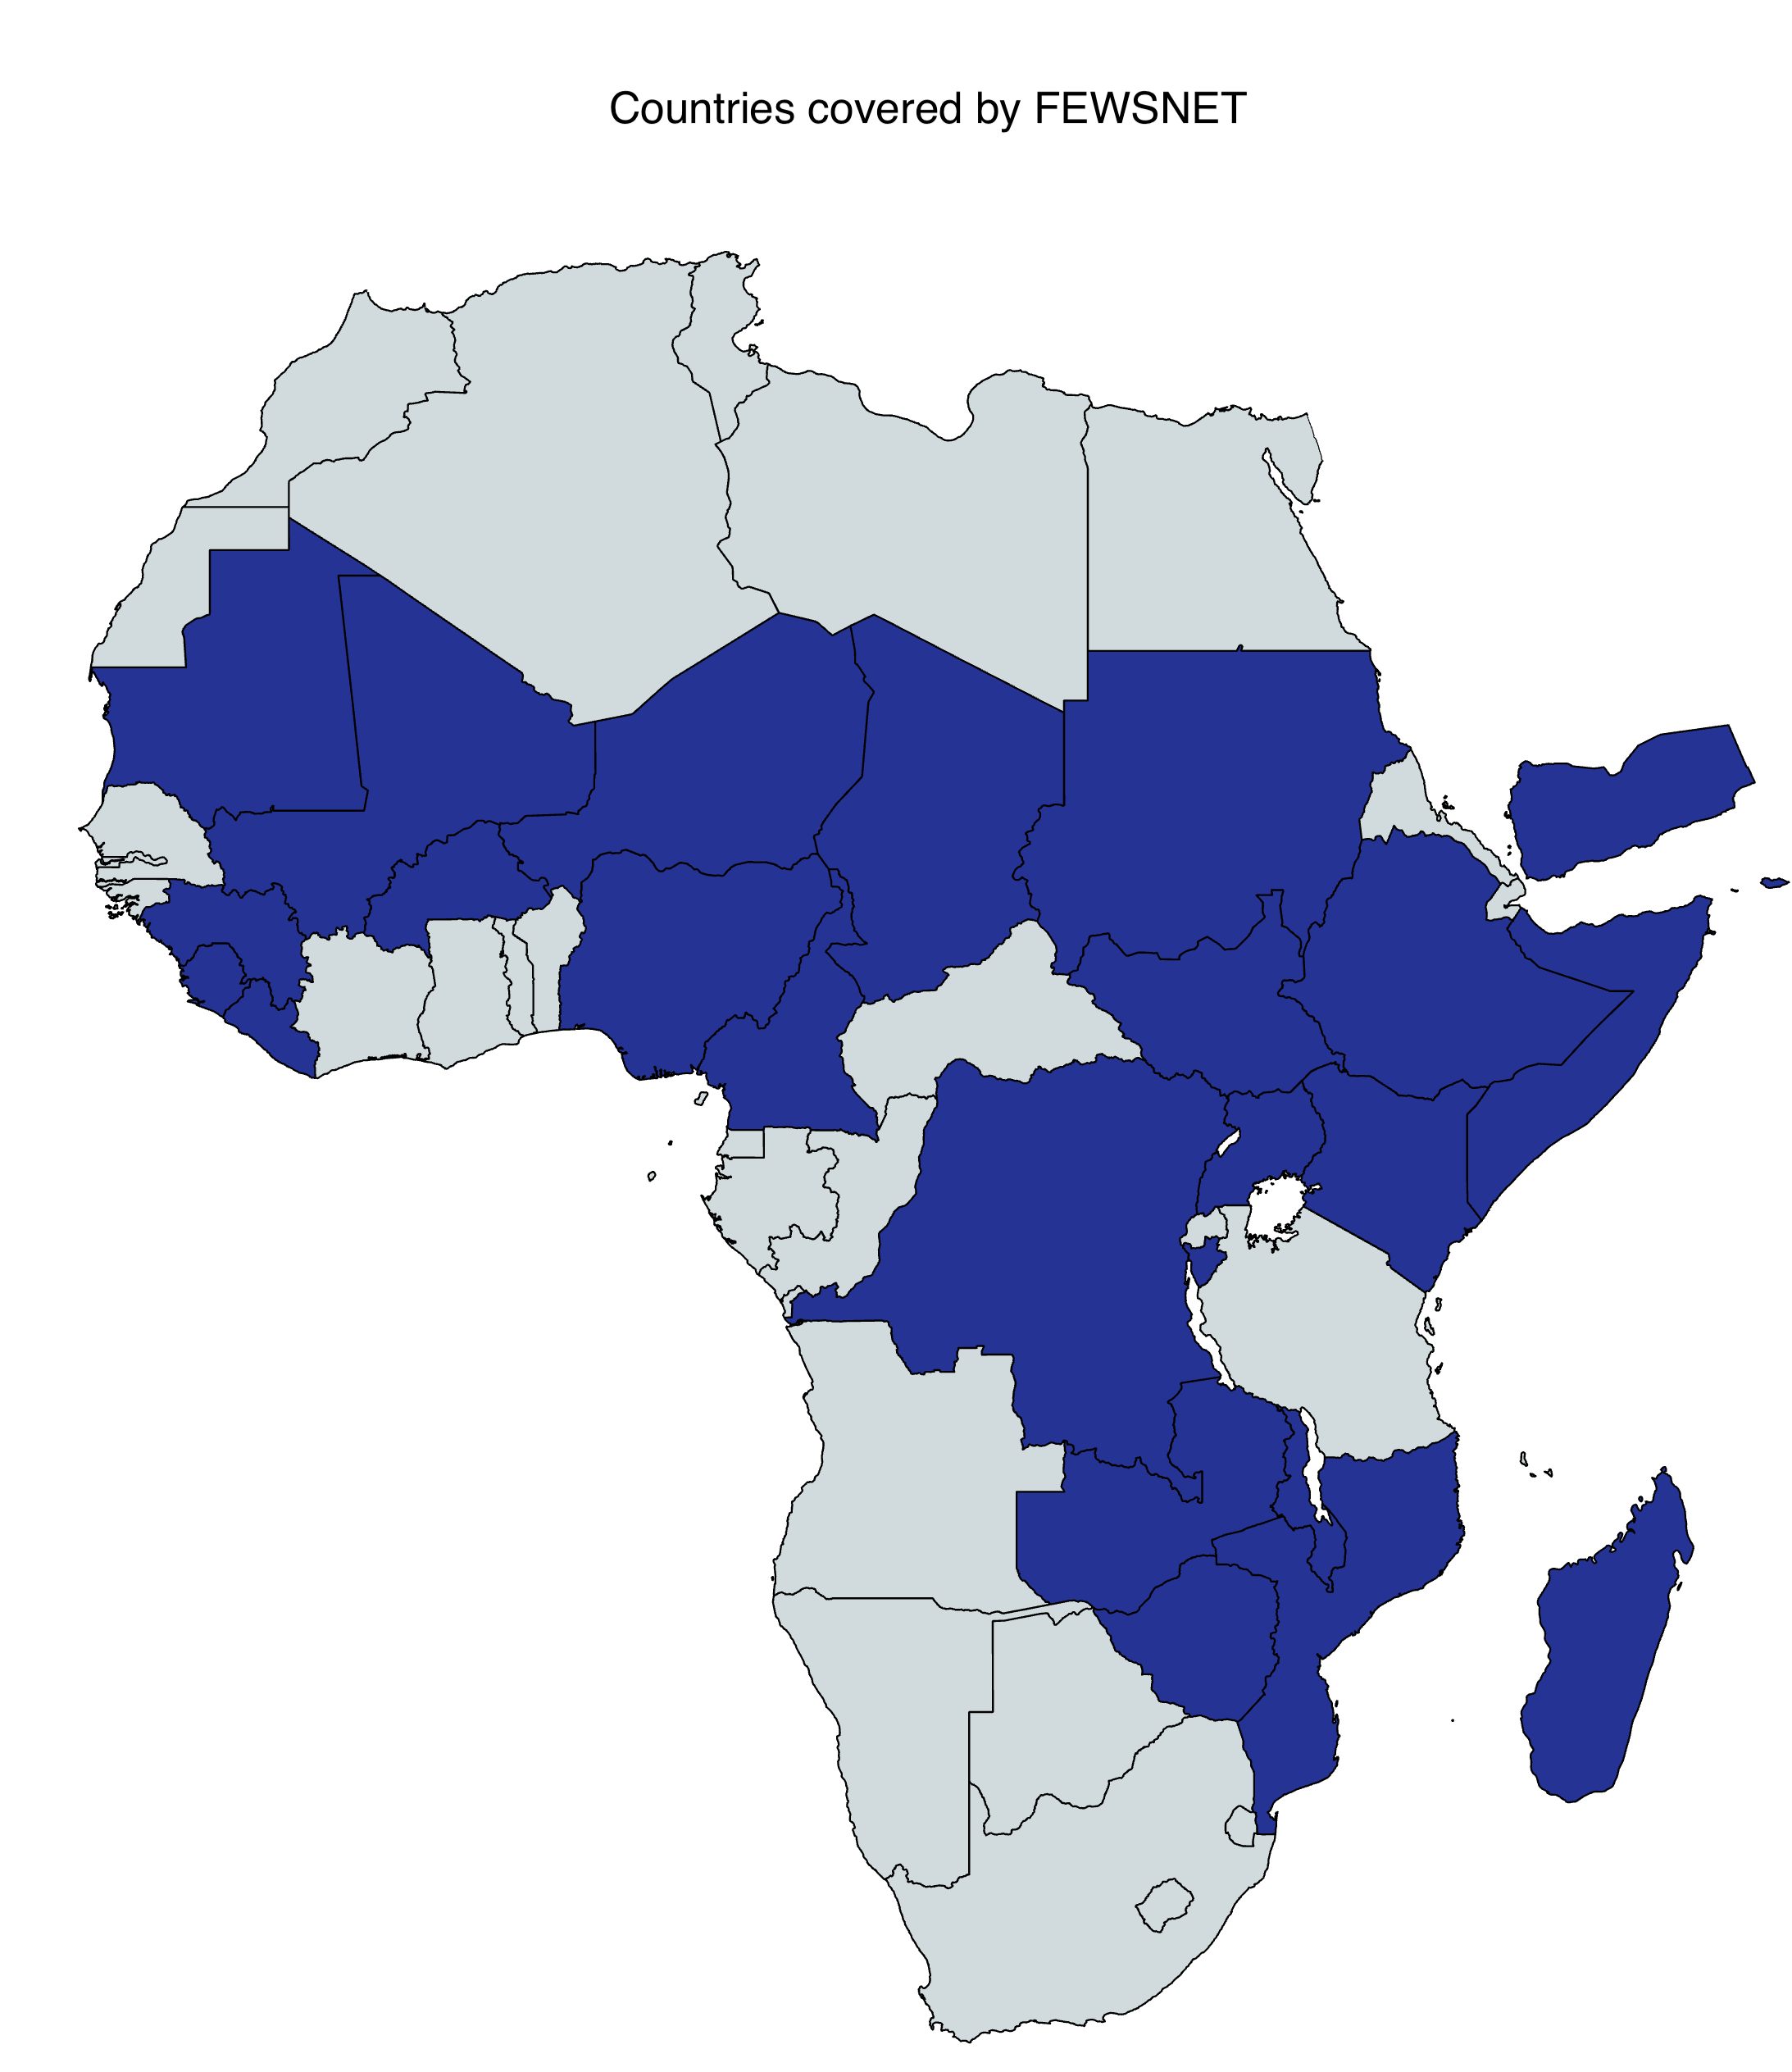
\includegraphics[width=0.8\textwidth]{map.png}
\captionsetup{labelfont=bf}
\caption{Countries in blue are those for which FEWS NET generates regular assessments. This study focuses on the African countries and Yemen.}
\label{fig:fewsnet_map}
\end{figure}

A central aspect of FEWS NET's methodology is its use of the Integrated Food Security Phase Classification (IPC), an international framework for categorising acute food insecurity into five ordinal phases \citep{ipc2019manual}. These range from Phase 1 (“Minimal”) to Phase 5 (“Famine”), with each level representing a progressively worse state of access to food.\footnote{In this paper, the terms “phase” and “class” are used interchangeably to refer to IPC levels, consistent with machine learning terminology.} The IPC framework provides a standardised vocabulary and visual schema for communicating food security severity across regions and time. Analysts assign phases to specific livelihood zones or administrative regions, based on a combination of primary and secondary data, field assessments, and scenario modelling. An overview of the five IPC phases is shown in Figure~\ref{fig:ipc_scale}.

\begin{figure}[ht]
\centering
\textbf{IPC Scale Overview}\par\vspace{0.5em}
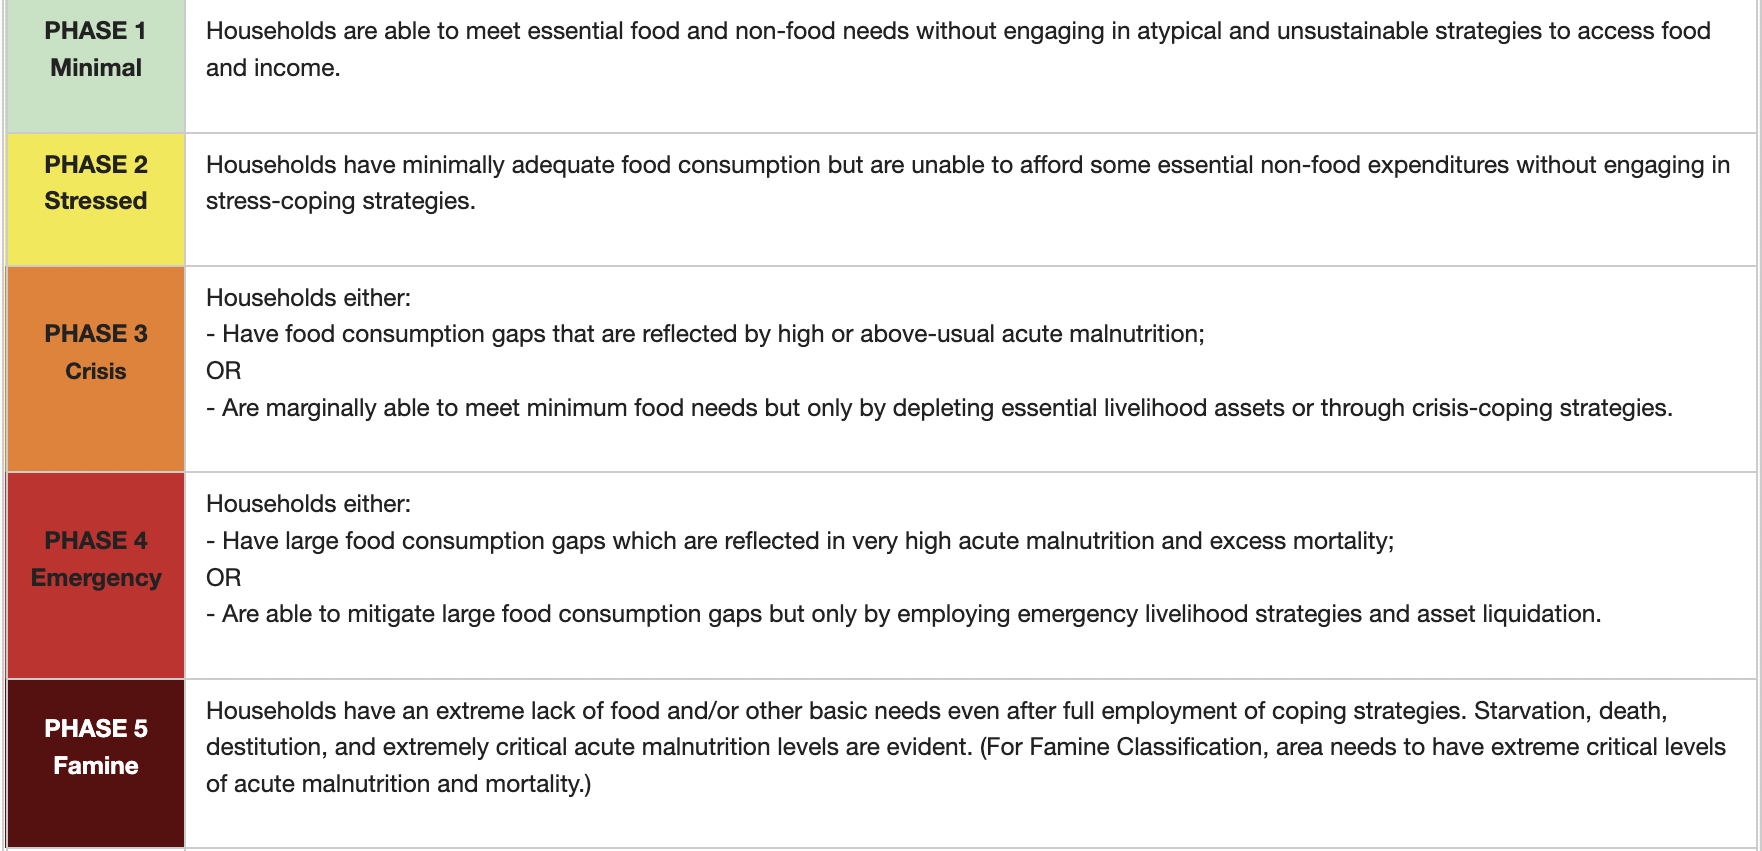
\includegraphics[width=\textwidth]{ipc_scale.png}
\caption{The five IPC phases used by FEWS NET to classify acute food insecurity. Source: FEWS NET.}
\label{fig:ipc_scale}
\end{figure}

With each publication cycle, FEWS NET releases the raw data behind each report, enabling researchers to conduct independent work on the FS topic. The key datasets made available, and those utilised in this study are the following:

\begin{itemize}
  \item \textbf{Food Security Classification}: Provides the IPC phase classification for each geographical area. Specifically, for this study we used the Current Situation (CS) assessment for the state of FS at the time of the reports' publication. Each file consists of one row for each of the 5 IPC FS phases, and each phase has a set of polygons associated to them, which allows to draw the different areas by their given state of FS phase;
  
  \item \textbf{Administrative Boundaries}: shapefiles containing polygons with information about sub-national level administrative boundaries, which are officially defined geographic divisions; 
\end{itemize}

In this study, we focus on FEWS NET’s \textit{Current Situation} (CS) phase maps, which describe food security conditions at the time of publication. These maps are released roughly three times per year—typically in February, June, and October—since the program’s shift in cadence in 2016. We limit our dataset to reports from 2016 onward to ensure temporal consistency in methodology and coverage~\citep{backer2021validating}. For each report, we extract geospatial shapefiles that contain polygons tagged with IPC phases. When multiple phases are reported for a given area, we select the highest (i.e., most severe) phase as the label for that region. We experimented with alternative aggregation strategies, including the mean and median phase, but found negligible differences in model performance. Moreover, such averages tend to flatten the distribution toward moderate categories, underrepresenting the most severe cases—which are precisely the outcomes of greatest operational and humanitarian relevance. We also use FEWS NET-provided administrative boundary files to align and aggregate data across time and countries. Our analysis includes all countries within FEWS NET’s African portfolio, as well as Yemen, which is treated as a regional priority due to its chronic crisis classification and operational significance (Figure~\ref{fig:fewsnet_map}).\\

While FEWS NET primarily serves policy and humanitarian actors, its high-quality spatial and temporal resolution makes it an attractive target for machine learning and predictive modelling. Recent studies have demonstrated how FEWS NET data can serve as training targets for AI systems. Fraiberger et al.~\citep{Fraiberger2023}, for instance, use FEWS NET IPC classifications as ground truth to train a multilingual NLP model that mines conflict- and climate-related signals from 11 million news articles. Their model, which learns to associate narrative signals with IPC outcomes, improved food crisis forecasting accuracy by over 40\% compared to baselines without textual features. Similarly, Westerveld et al.~\citep{westerveld2021forecasting} train a gradient boosting model using over 130 input variables—including weather anomalies, prices, and prior IPC values—to predict transitions in food security states in Ethiopia. Their system achieved strong skill in forecasting both improvements and deteriorations several months in advance. These efforts show how FEWS NET’s IPC data can be leveraged as structured, expert-labelled outcomes for training scalable, automated early warning systems \citep{michelson2023mlfs}.\\

Together, these insights affirm the utility of FEWS NET’s IPC outputs not only as operational decision-support tools, but also as a benchmark for scientific inquiry into food security prediction and nowcasting.

\subsubsection{GDELT Data}

The \textit{Global Database of Events, Language, and Tone} (GDELT) is an open-source platform for near-real-time monitoring of socio-political events and media narratives worldwide. It continuously ingests news reports from nearly every country in over 100 languages \citep{gdeltproject,leetaru2013gdelt}, cataloguing events and topical content as they unfold. GDELT thus provides a massive open dataset of structured information on global happenings at fine temporal granularity.

\paragraph{GDELT Events.}
The GDELT \textbf{Event} database records discrete events in the news using a “who did what to whom” schema. Each event entry includes an \textit{Actor1} (initiator) and \textit{Actor2} (target), which can be individuals, organizations, or countries, along with a CAMEO event code classifying the type of action (based on the Conflict and Mediation Event Observations taxonomy) \citep{leetaru2013gdelt}. These CAMEO codes range from cooperative to conflictual event types and enable systematic analysis of event categories. Each event record is annotated with the event’s date/time and location, the number of news articles that reported on it, and an average sentiment (“Tone”) score. A Goldstein scale value is also provided to estimate the event’s potential impact on stability.

\paragraph{Article retrieval and filtering (Events).}
While GDELT provides structured metadata and event annotations, the full news article texts are not directly included and must be retrieved separately. For the GDELT Events stream, we downloaded and consolidated all event records covering January~2016 to February~2024, yielding approximately four million event-linked article references prior to text-level processing. From the consolidated dataset, we extracted all unique \texttt{SOURCEURL} entries associated with events geolocated to FEWS~NET administrative areas, resulting in roughly 1.9~million distinct URLs. Each URL was retrieved by directly scraping the corresponding webpage using a high-concurrency pipeline with retries and timeouts. After scraping, we excluded noisy or analytically irrelevant events by removing selected CAMEO categories, reducing the corpus to approximately 920{,}000 articles. We then applied a domain-specific food-security lexicon, reducing the dataset to around 381{,}000 articles. Following heavy text preprocessing, truncation to 500 words, and near-duplicate removal using MinHash-based similarity, the final Events-based corpus comprised approximately 350{,}000 unique news articles.

\paragraph{GDELT Global Knowledge Graph.}
Complementing the event data, the GDELT \textbf{Global Knowledge Graph (GKG)} operates at the article level and captures the surrounding context and content of news articles. For each article, it extracts mentioned locations, persons and organizations, thematic keywords, numeric quantities (e.g.\ casualties, prices, aid amounts), prominent quotes, and an overall sentiment score. In sum, the GKG provides a detailed snapshot of actors, issues, and tone in media narratives.

\paragraph{Article retrieval and filtering (GKG).}
For the GDELT Global Knowledge Graph, we followed a parallel pipeline adapted to its article-centric structure. Daily GKG files were aggregated and consolidated before being spatially mapped to FEWS~NET administrative units. From the resulting dataset, we extracted all unique article URLs listed in the \texttt{DocumentIdentifier} field, after normalisation and removal of malformed entries. These URLs were scraped individually using the same chunk-based, fault-tolerant framework employed for the Events data. In contrast to the Events stream, GKG records are already thematically filtered through GDELT’s count- and topic-based annotations. We nevertheless applied additional cleaning steps to remove duplicates and empty or non-textual pages. The resulting GKG article corpus---smaller than the Events corpus but richer in semantic annotations---was retained for downstream aggregation of keyword counts, aid mentions, and sentiment-linked indicators.


\subsection{Methodology}
\label{sec:methodology}

The overall data processing pipeline integrates food security outcome data from FEWS~NET with a rich array of features derived from GDELT's event database and Global Knowledge Graph (GKG). In summary, we align the FEWS~NET Integrated Phase Classification (IPC) labels with spatio-temporal features computed from GDELT, including event counts, news article frequencies, NLP-extracted signals, and keyword-based indicators. Below, we detail each step of this pipeline, from data alignment through feature extraction and model development, to ensure reproducibility and clarity.

\subsubsection{Data Pipeline and Alignment}
FEWS~NET (Famine Early Warning Systems Network) publishes sub-national food security assessments in the form of IPC phase classifications, which range from Minimal food insecurity (Phase~1) to Famine (Phase~5) \citep{ipc2019manual}. Our first step was to integrate these FEWS~NET IPC data with the GDELT dataset. GDELT (Global Database of Events, Language, and Tone) is an open-source global event database that codifies daily news events with geopolitical significance \citep{leetaru2013gdelt}. We obtained GDELT 2.0 data streams corresponding to two components: (1) the Event database of socio-political events (with CAMEO event coding), and (2) the GKG, which indexes news media content (identifying themes, locations, counts of keywords, etc. for each news article). \\

Because the two data sources differ in granularity, we performed careful geographic and temporal alignment. Geographically, we mapped GDELT records to FEWS~NET regions. FEWS~NET IPC analyses provide sub-national and national food security phase labels. To align with GDELT data, we aggregate all media-derived signals at standardized administrative levels (primarily ADMIN2 and country) rather than at livelihood zone boundaries, which are not directly used in the final modelling pipeline. To accurately assign GDELT events or articles to the corresponding FEWS~NET regions, we leveraged the location metadata available in GDELT, including country and administrative division names as well as latitude/longitude coordinates. For precise sub-national matching, we utilized administrative boundary data from the GADM database (\url{https://gadm.org/}), which provides comprehensive and standardized geographic shapefiles down to district levels. This mapping process used available latitude–longitude coordinates for spatial attribution by overlaying points on GADM shapefiles. When precise coordinates were unavailable or ambiguous, location was inferred using administrative names or country-level identifiers provided by GDELT. As a result, while many records could be attributed to second-level administrative units, others were assigned to broader administrative regions. Temporally, we aggregated all GDELT events and articles into year-month bins. This monthly temporal resolution provides a consistent indexing structure while aligning closely with the reporting intervals of FEWS~NET IPC assessments, which typically occur several times per year. All GDELT events and articles were thus binned by their publication date into year-month periods, and then aligned to the month of the FEWS~NET food security classification label for the same region. This yielded a unified dataset indexed by region and month, with the response variable being the FEWS~NET IPC phase and dozens of candidate predictor features from GDELT.\\

While our original motivation considered mapping news-derived signals to highly granular livelihood zones to reflect localized vulnerability (e.g., crop-specific impacts within a district), this proved challenging in practice. Open-source media data are often sparse and ambiguous at fine spatial scales, with many regions lacking sufficient coverage to support reliable signal extraction. Moreover, even when detailed agricultural or weather impacts are mentioned, they rarely map cleanly to specific livelihood zones in a way that meaningfully improves predictive performance. To balance spatial specificity with signal robustness, we therefore aggregate all GDELT-derived features at the second-level administrative unit (ADMIN2) by month, which offers a standardized and interpretable spatial resolution aligned with FEWS~NET IPC reporting.

\subsubsection{GDELT Events Filtering and Aggregation}

From the GDELT Events database, we extracted records associated with humanitarian action, conflict dynamics, and socio-political activity using CAMEO event codes. Rather than restricting analysis to a single event category, we considered a broad set of codes capturing humanitarian assistance, protest, violence, coercion, and economic support, including but not limited to codes for provision of aid, protest actions, assault and fight events, economic aid appeals, and related categories.

Each event record in the GDELT Events stream includes geographic information (latitude and longitude when available, and administrative names). We mapped these records to second-level administrative units (ADMIN2) when possible using GADM shapefiles; when precise coordinates were unavailable or ambiguous, we relied on country-level location identifiers provided by GDELT. Temporal aggregation was performed on a monthly basis by binning event dates into year-month periods. From these processed records, we derived a set of event-based features for each ADMIN2–month unit (or country–month where finer attribution was unavailable), including distinct event counts, total event mentions, and the number of unique sources reporting events within that period.

\subsubsection{GDELT GKG Filtering and Aggregation}

In parallel, we extracted thematic signals from the GDELT Global Knowledge Graph (GKG), which encodes article-level metadata including thematic tags and numeric counts related to various content categories. We filtered GKG records using comprehensive thematic codes and keywords associated with food security, conflict, economic conditions, natural hazards, and health and sanitation. Key thematic filters included labels such as \texttt{FOOD\_SECURITY}, agriculture-related tags, conflict/security indicators, economic shock themes, and weather- and hazard-related codes.

Geographic attribution for GKG records utilized the primary location identified by GDELT; this often corresponds to country-level identifiers and, when available, second-level administrative units. As with Events data, records were temporally aggregated into year-month periods. From these aggregated GKG records, we constructed thematic count features by leveraging the V2Counts field where numeric indicators were available (e.g., counts of fatalities or displaced people) and frequency-based indicators for theme mentions otherwise. For each ADMIN2–month unit (or country–month where finer resolution was unavailable), we also computed article-level media attention measures reflecting the volume and thematic composition of coverage relevant to humanitarian and food security contexts.


\subsubsection{NLP-Based Article Classification (MultiTaskBERT)}
While the thematic article counts provide quantitative measures of coverage, we further enriched the textual data through natural language processing. We collected the full text (or summaries where full text was unavailable) of the news articles identified in the previous step and subjected them to a multi-label classification analysis to extract deeper semantic signals. We developed a custom \textbf{MultiTaskBERT} model, built on the BERT transformer architecture \citep{devlin2019bert}, to simultaneously classify each article along multiple dimensions relevant to humanitarian analysis:
\begin{itemize}\itemsep0em 
    \item \textbf{Impact Type}: the general category of crisis or impact described (e.g., conflict-related, weather shock, health epidemic, economic downturn, etc.).
    \item \textbf{Urgency}: the immediacy or severity of the situation, indicating whether the article describes an ongoing emergency, an emerging threat, or a longer-term concern.
    \item \textbf{Mentioned Resources}: the types of relief or resources involved, such as food assistance, nutrition supplements, water/sanitation, medical supplies, or livelihood support.
\end{itemize}
Using a single BERT-based model for all three tasks allowed us to employ a hard parameter-sharing multi-task learning approach: the model has one shared encoder (the BERT backbone) with separate output layers (classification heads) for each task. This design exploits commonalities in language cues across tasks (for example, the words indicating urgency might also inform the type of impact).

For training the multi-task classifier, we constructed a labeled corpus of 7{,}000 humanitarian news articles. Each article in the training set was annotated with the appropriate impact type label, an urgency level, and the resource categories mentioned. Due to resource constraints, we did not produce a fully human-annotated training set. Instead, we adopted a \textit{weak supervision} approach in which the training labels were generated by a large language model (OpenAI's GPT-5.1), prompted with task-specific instructions and few-shot examples for each classification dimension. We treat these as \textit{silver-standard} rather than gold-standard labels and flag two consequences explicitly. First, any systematic biases or blind spots of the labelling model (for example, language, regional, or framing biases in how humanitarian impact and urgency are interpreted) can propagate into the BERT classifier trained on them, and ultimately into the downstream features. Second, our validation of these labels is limited: a random 5\% subset was manually reviewed by the authors, and while this spot-check indicated high agreement with the LLM-generated labels, it is a small, non-independent audit rather than a rigorous inter-annotator study against an external gold standard. The resulting MultiTaskBERT outputs should therefore be read as informative but noisy intermediate signals rather than validated ground truth, and a larger human-labelled corpus with formal agreement metrics remains important future work. In preprocessing, we applied BERT’s WordPiece tokenization to each article’s text, ensuring consistency with the model’s vocabulary. Many articles were longer than BERT’s maximum sequence length of 512 tokens; to address this, we employed a \textbf{sliding window} tokenization strategy. Specifically, long texts were split into overlapping segments of up to 512 tokens (with a stride, e.g. 256, to retain context between segments). Each segment was fed through the model, and we aggregated the segment-level predictions (using either averaging or taking the most severe category) to produce article-level classifications. This sliding window approach preserved as much information as possible from lengthy reports while respecting BERT’s input size constraints.\\

We partitioned the data into training and validation sets using stratified sampling, so that each class (for each task) was proportionally represented in both sets. This \textbf{stratified split} was important to prevent minor classes (such as less common impact types or resource categories) from being absent in the validation fold. The MultiTaskBERT model was implemented in PyTorch, using the Hugging Face Transformers framework. We leveraged Hugging Face’s \textbf{Trainer API} to manage the training loop, which provided features like dynamic learning rate scheduling, gradient accumulation for long sequences, and periodic evaluation on the validation set. During training, the model’s loss was computed as the weighted sum of the losses of the three classification heads: two heads used standard cross-entropy loss (for impact type and urgency classification), and one head used binary cross-entropy loss (for the multi-label resource classification task). We adjusted task-specific loss weights to balance the influence of each task, given that the number of classes and label frequencies differed by task. As training progressed, we monitored performance using standard classification metrics including accuracy and macro-averaged F1 score for each task. The final MultiTaskBERT model achieved validation accuracy of approximately 0.75 for impact-type classification and 0.79 for urgency classification, and macro-averaged F1 scores of 0.84 for resource identification, indicating that it learned to extract the targeted information from news text with reasonable accuracy across all three tasks. We selected the checkpoint at the end of training (epoch~10), as resource F1 continued to improve throughout; full per-epoch metrics are reported in the appendix (Table~\ref{tab:bert_training_metrics}). After training, we used this model to infer labels on all relevant GDELT articles in our dataset. Each article thus received an \textit{impact type}, an \textit{urgency level}, and a set of \textit{resource mentions} as predicted by the model. We aggregated these outputs to create additional region-month features: for example, the number of articles in a region-month classified as “high urgency,” the count of articles mentioning food or water resources, or the distribution of impact types (how many articles were conflict-related vs. climate-related, etc.). These features provide a nuanced textual summary of the humanitarian situation reported in the news for each region and time period. \\

\subsubsection{Keyword-Based Textual Feature Extraction}
To complement the model-driven NLP features, we also implemented a rule-based textual analysis to capture specific crisis indicators that might be explicitly mentioned in news articles. In particular, we were interested in quantifying references to \textbf{fatalities}, \textbf{displacement}, and \textbf{economic shocks} in the news, as these are key aspects of humanitarian crises (e.g. casualty counts, population movements, market disruptions). Some of these signals are directly available from GDELT’s metadata: the GKG includes a structured \textit{V2Counts} field which enumerates numeric counts reported in the text for a predefined set of categories (e.g., the number of people killed, number of people displaced, number injured or sick, etc.). We leveraged these GDELT-provided counts when available. For instance, if an article’s GKG record indicated \texttt{CountType=KILL} with a Number value, we took that as the reported fatalities in that article. Likewise, \texttt{CountType=DISPLACED} (or related types covering refugees) gave us the number of people displaced. These pre-extracted features from GDELT (the ``V2Counts’’ fields) were incorporated as article-level data points and subsequently aggregated per ADMIN2–month (or higher where finer resolution was unavailable) (summing the totals or taking the maximum, as appropriate, to reflect the scale of impact mentioned in that month).\\

However, not all relevant textual cues are captured by GDELT’s predefined counts, especially for economic shocks or more nuanced context. Therefore, we developed custom scripts to scan the article texts for additional keywords and patterns. We compiled domain-specific lexicons for each category of interest. For fatalities, the lexicon included words and phrases like “killed,” “deaths,” “casualties,” “fatalities,” as well as contextual phrases (e.g., “people killed,” “dead bodies”) to reduce false positives. For displacement, we listed terms such as “displaced,” “homeless,” “evacuated,” “refugees,” “internally displaced persons (IDPs),” etc. For economic shocks, we gathered keywords relating to market and livelihood crises: e.g., “prices,” “inflation,” “drought” (as an economic shock to agriculture), “unemployment,” “loss of income,” “economic crisis,” and so forth. Using these lexicons in combination with regular expressions, we performed a scan on each article’s text. We utilized the spaCy NLP library to assist with this process: spaCy’s tokenizer and part-of-speech tagger helped us identify keyword instances in context and to capture numeric modifiers. For example, if the word “displaced” appeared, our script would look to its immediate left for a number (e.g., “50{,}000 displaced”) or a quantifier phrase (like “thousands of people displaced”) and extract that quantity if present. Regular expressions were used to reliably find patterns like “[0-9,]+ (people )?killed” or “million people displaced,” etc. This approach allowed us to quantify not just the presence of a keyword but the magnitude of the reported phenomenon when available. In cases where a numeric figure was not explicitly given (e.g., “many people were displaced”), we instead marked a boolean flag that the article mentioned displacement qualitatively.\\

From this textual analysis, we derived several features per article: the number of fatalities mentioned (if any), the number of people displaced, an indicator of any economic shock mention, and counts of economic-related terms (for instance, how many different economic shock terms were present, as a simple proxy for economic stress). These article-level features were then aggregated to the administrative-unit–month level. We took sums for additive quantities (e.g., total fatalities mentioned in all articles that month for the district) and counts of articles for qualitative indicators (e.g., how many articles in the administrative-unit–month mentioned any displacement, serving as a frequency indicator of displacement-related news). The outcome of this step was a set of structured features capturing the crisis impacts described in the news text, derived via lexicon- and regex-based mining. Combining both the GDELT V2Counts data and our custom extraction ensures we did not miss crucial signals simply because they were not covered by the default GDELT schema. This multi-pronged text analysis is especially valuable for capturing aspects like \textbf{conflict intensity (fatalities)} or \textbf{population movement (displacements)} that directly inform food security outcomes (e.g., conflict fatalities may disrupt food systems, and mass displacement often leads to humanitarian emergencies).

\subsubsection{Model Training and Evaluation}
The final stage of our methodology was to merge all the engineered features with the outcome labels and train predictive models to forecast food insecurity. By the end of the data processing pipeline, for each administrative-unit–month we have: the FEWS~NET IPC label (our ground-truth indicator of food security status), and a rich feature vector drawn from GDELT (including event counts, article counts, NLP-derived features, and keyword-based metrics). We constructed a modelling dataset from 2016 through 2024 (covering all available overlapping time periods between GDELT and FEWS~NET data), totalling approximately 71{,}000 administrative-unit–month examples. Prior to modelling, all features were standardized (when required for certain algorithms) and we applied any necessary imputation for missing values (e.g., if a region had no news articles in a month, the corresponding features were set to zero).\\

In order to properly quantify the impact of the features we have extracted, we established four baseline models. All four are constructed with the goal of predicting future Food Security (FS) states at the district level. The first three baselines rely on simple heuristic rules, detailed below, applied directly to FEWS NET's historical FS data. These heuristics are designed to capture patterns that may recur periodically over time—what we refer to as "seasonal" and "recurring" patterns. In this context, "seasonal" refers to any cyclical trend or repeated pattern observed in the data. \\

The fourth baseline moves beyond heuristics and employs a machine learning (ML) approach. By using historical FS states as input variables, this model can identify complex relationships and subtle patterns that simple heuristics might miss. As a result, the ML-based model has the potential to improve both the modelling process and the accuracy of predictions, providing more robust insights to guide decision-making and interventions. \\

Since the goal of this paper is to quantify both the added value and the substitutability of features extracted from news data in predictive food security models, such data were not included in any of the baselines.

Below is a detailed description of each baseline we have computed:
\begin{itemize}

\item \textbf{Previous Period's IPC Score (PPS)}: This first model assumes a scenario of no change in food security conditions and simply replicates the Integrated Food Security Phase Classification (IPC) score from the preceding period. Its aim is to provide insights into the stability of food security over consecutive periods.

\item \textbf{Same Period Last Year (SPLY)}: Recognizing the influence of seasonal factors on food security, this model considers the IPC score from the same period in the previous year. By accounting for seasonality, its aim is to capture recurring patterns and provide insights into cyclical trends in food security.

\item \textbf{Maximum of Previous Two Periods (Max-2PP)}: This model selects the highest (worst) IPC score from the previous two periods. Its aim is to highlight potential deteriorations by reflecting on recent negative trends in food security conditions.

\item \textbf{Classifier using historical CS scores (CHS)}: This ML model was trained using exclusively the most recent IPC Current Situation score (forward-filled) and geographic dummy variables encoding the administrative region (ADMIN0/ADMIN1/ADMIN2). It serves as an ML baseline that measures how well standard classifiers perform with lagged IPC scores and location context alone, before any GDELT-derived features are introduced.
\end{itemize}

After establishing baseline performance, we trained three ML classifiers across multiple feature configurations: \textbf{Logistic Regression} (LR), \textbf{Random Forest}~\citep{breiman2001random} (RF), and \textbf{CatBoost}~\citep{dorogush2018catboost}. These models span a range of modelling paradigms, from a regularised linear model to tree-based ensembles capable of capturing nonlinear interactions, while balancing interpretability and predictive power. We deliberately excluded deep learning architectures (e.g., LSTMs, feed-forward neural networks) from the prediction stage: the relatively modest number of input features limits the advantage of such models over gradient-boosted trees, and their reduced interpretability would hinder the diagnostic goals of this study. Features were standardised when required (for LR), and tree-based models received raw feature values. We treated the prediction problem as a multi-class classification (predicting the IPC phase 1--5). Model evaluation followed a \textbf{rolling temporal window} protocol designed to mimic realistic operational forecasting. For each IPC assessment period in the evaluation set, models were trained on data from the preceding 20 monthly periods and tested on the held-out assessment period. This forward-chaining scheme ensures strict temporal separation between training and test data, preventing look-ahead bias while reflecting the sequential nature of food security monitoring.\\

We evaluated all models using accuracy and the macro-averaged F$_1$ score, which weights all classes equally to ensure that minority outcomes (particularly higher IPC phases) are properly represented. To assess sensitivity to temporal coverage, we reported results for two evaluation scopes: the full set of available assessment periods (25 evaluations, 2016--2024) and a recent subset (last 6 evaluations, 2022--2024), motivated by documented improvements in GDELT's geographic coverage and source diversity over time.

We also analysed feature importance scores from Random Forest models to identify which GDELT-derived signals were most informative for prediction.\\

In summary, our methodology starts with merging FEWS~NET IPC labels with GDELT Event and GKG data, followed by diagnostic comparison of both streams and multi-step feature engineering—including event filtering by CAMEO code (e.g., 073 for humanitarian aid), thematic article counts (food security themes), NLP-based text classification (via a multi-task BERT model predicting impact, urgency, and resource needs), and lexicon- and regex-based keyword extraction (capturing fatalities, displacement, economic shocks, etc.). Based on the diagnostic finding that GKG coverage is too spatially sparse for sub-national modelling, the predictive models use only GDELT Events-derived features. This design allows us to rigorously test whether open-source event and news data can serve as reliable, interpretable, and timely proxies for on-the-ground food security outcomes—potentially advancing near-real-time food security monitoring in resource-constrained settings.

\section{Results}
We begin by examining country-level media coverage across Africa and Yemen using the two GDELT products (Figure~\ref{fig:gdelt_maps}). Both datasets provide broad geographic coverage across FEWS NET countries, although several states appear with no records in at least one source, highlighting non-random gaps in media reporting. Despite this overlap in coverage, the spatial distribution of article volumes differs markedly between datasets. The Events database exhibits strong cross-country heterogeneity, with a small number of countries, most notably Nigeria, Ethiopia, and Sudan, showing very high article counts relative to the rest of the continent. In contrast, the GKG data display a more compressed distribution, with many countries clustered at intermediate levels of coverage and fewer extreme values. One clear exception is Yemen, which appears as a pronounced outlier in the GKG map, reflecting sustained international media attention and the narrative richness captured by article-level knowledge graphs rather than discrete event coding. Taken together, these patterns suggest that while both GDELT sources offer extensive geographic reach, they encode fundamentally different dimensions of information: event intensity versus narrative salience.\\

Extending the analysis along the temporal dimension, we aggregated GDELT article counts by country and by month (Figure~\ref{fig:gdelt_temporal}). At this level of granularity, both datasets retain a skew toward a subset of highly covered countries, but they differ markedly in their temporal structure. The Events dataset is characterised by relatively stable baseline coverage punctuated by sharp, short-lived spikes that align closely with discrete episodes of violent conflict. A prominent example is Sudan, where article counts surge abruptly from April~2023 onward, coinciding with the outbreak of large-scale fighting between the Sudanese Armed Forces and the Rapid Support Forces, which rapidly escalated into a nationwide humanitarian emergency \citep{reuters_sudan_2023, unocha_sudan_2023}. A similar, though more localized, spike is observed for Niger in August~2023, following the July military coup and subsequent intensification of insurgent attacks in the Tillabéri region \citep{reuters_niger_2023, icg_niger_2023}.\\

In contrast, the GKG dataset exhibits a smoother but more strongly time-skewed distribution, with article volumes increasing substantially from 2023 onward across several countries. This pattern is especially pronounced for Yemen and Sudan, reflecting sustained international media attention to protracted conflicts, humanitarian access constraints, and diplomatic developments rather than isolated violent events \citep{reuters_yemen_2023, unocha_yemen_2023}. Smaller but noticeable increases in GKG coverage are also visible for countries such as Mauritania in mid-2023, plausibly linked to nationally salient political events, including legislative elections, though without the acute crisis signals observed in active conflict settings \citep{africanews_mauritania_2023}. Overall, these temporal patterns highlight a fundamental distinction between the two GDELT products: Events data respond sharply to episodic shocks, while GKG data accumulate more gradually as narrative intensity builds over time.

\begin{figure}[H]
    \centering
    % GDELT Events
    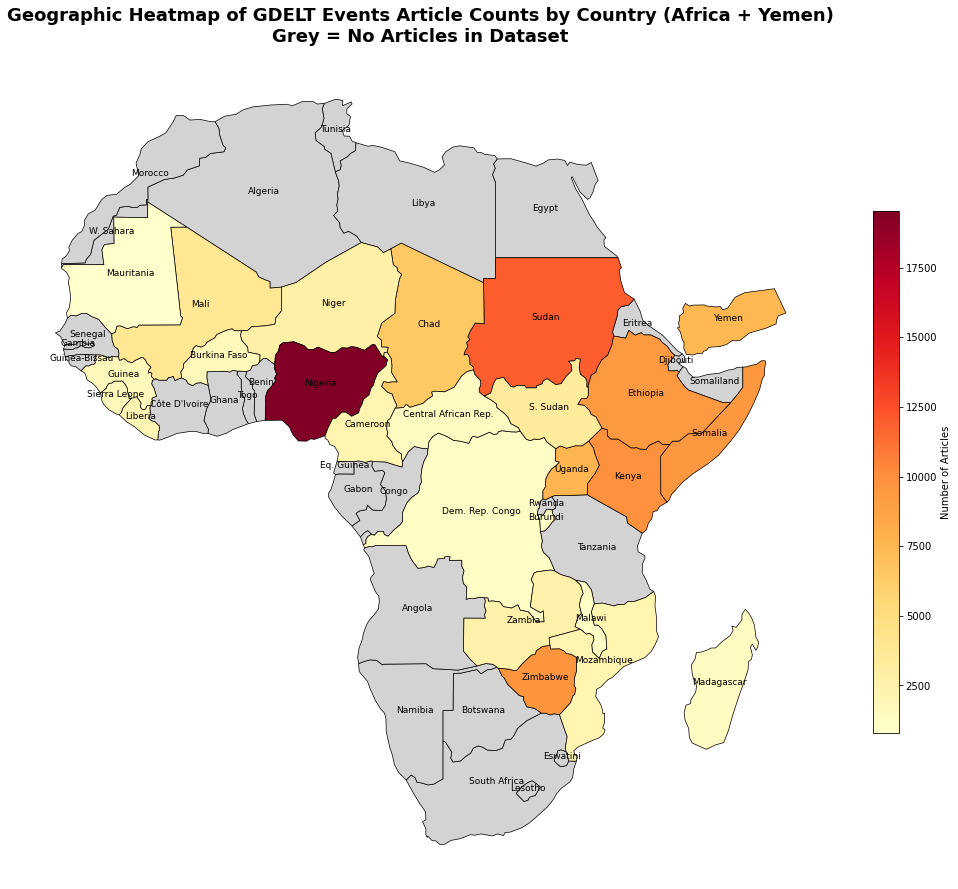
\includegraphics[width=0.6\textwidth]{events_map.png}

    \vspace{0.5em}

    % GDELT GKG
    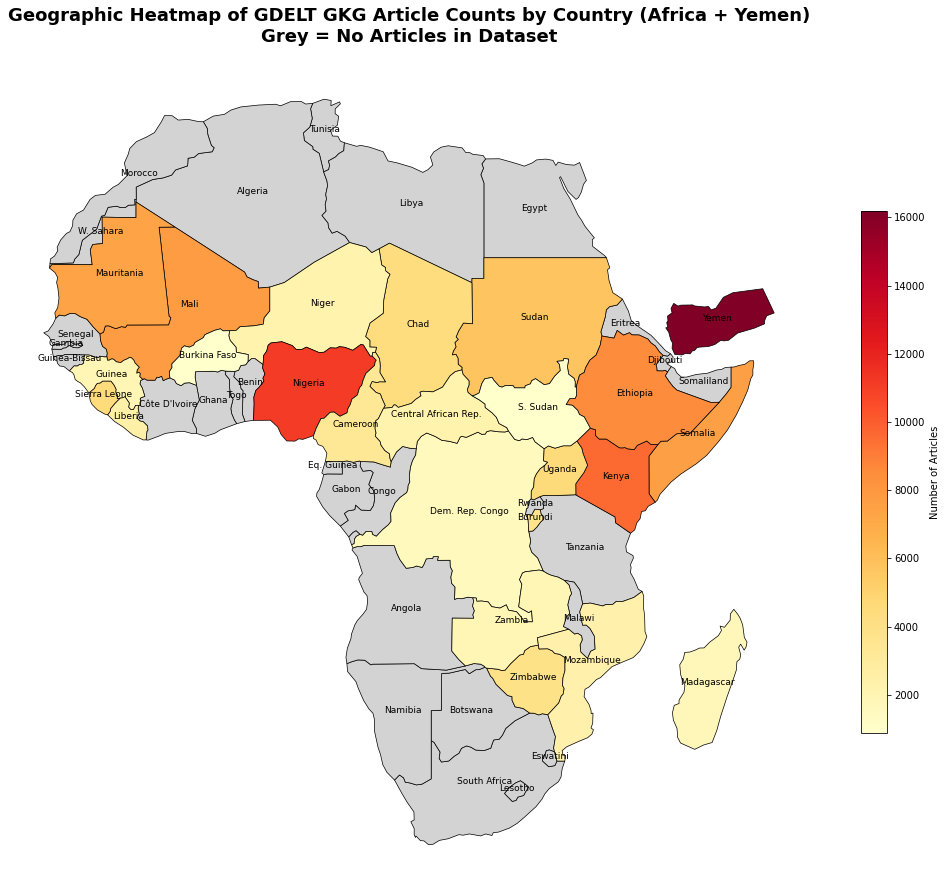
\includegraphics[width=0.6\textwidth]{gkg_map.png}

    \caption{Geographic distribution of GDELT article coverage across Africa and Yemen.
    \textbf{Top:} GDELT Events article counts, reflecting the spatial distribution of reported events.
    \textbf{Bottom:} GDELT Global Knowledge Graph (GKG) article counts, capturing narrative-based media coverage.
    Grey shading indicates countries with no articles in the corresponding dataset.}
    \label{fig:gdelt_maps}
\end{figure}



\begin{figure}[tbp]
\centering
% Top: GDELT Events (smaller height)
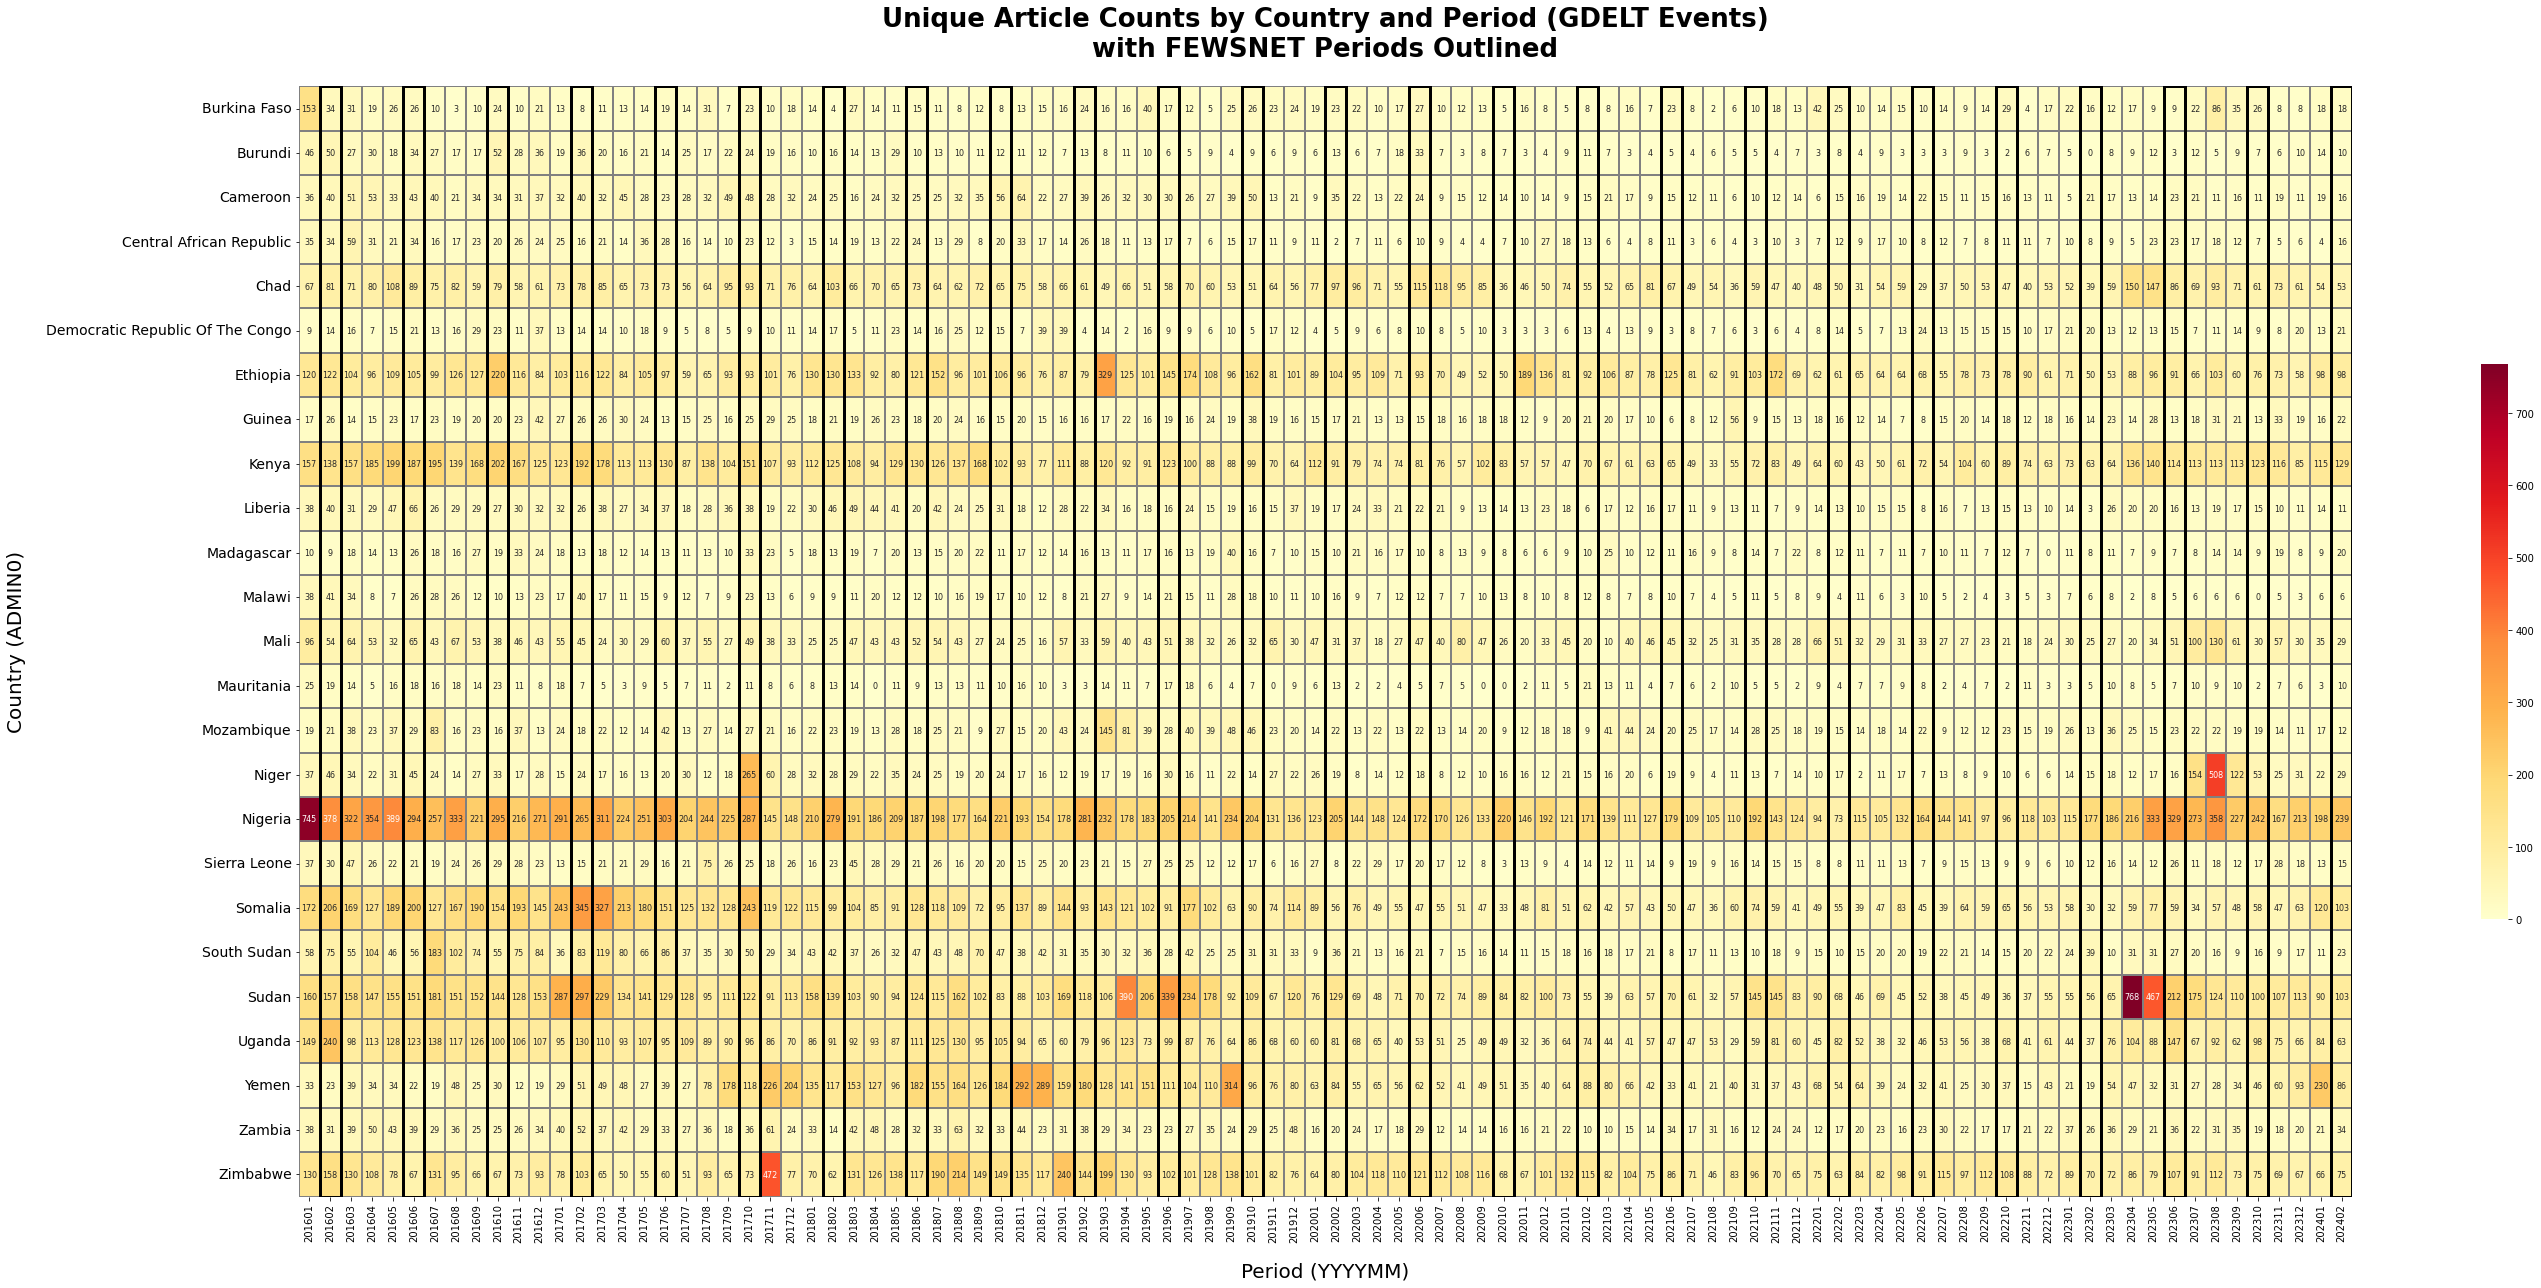
\includegraphics[width=1\textwidth]{events_article_counts.png}
\vspace{0.8em}
% Bottom: GDELT GKG
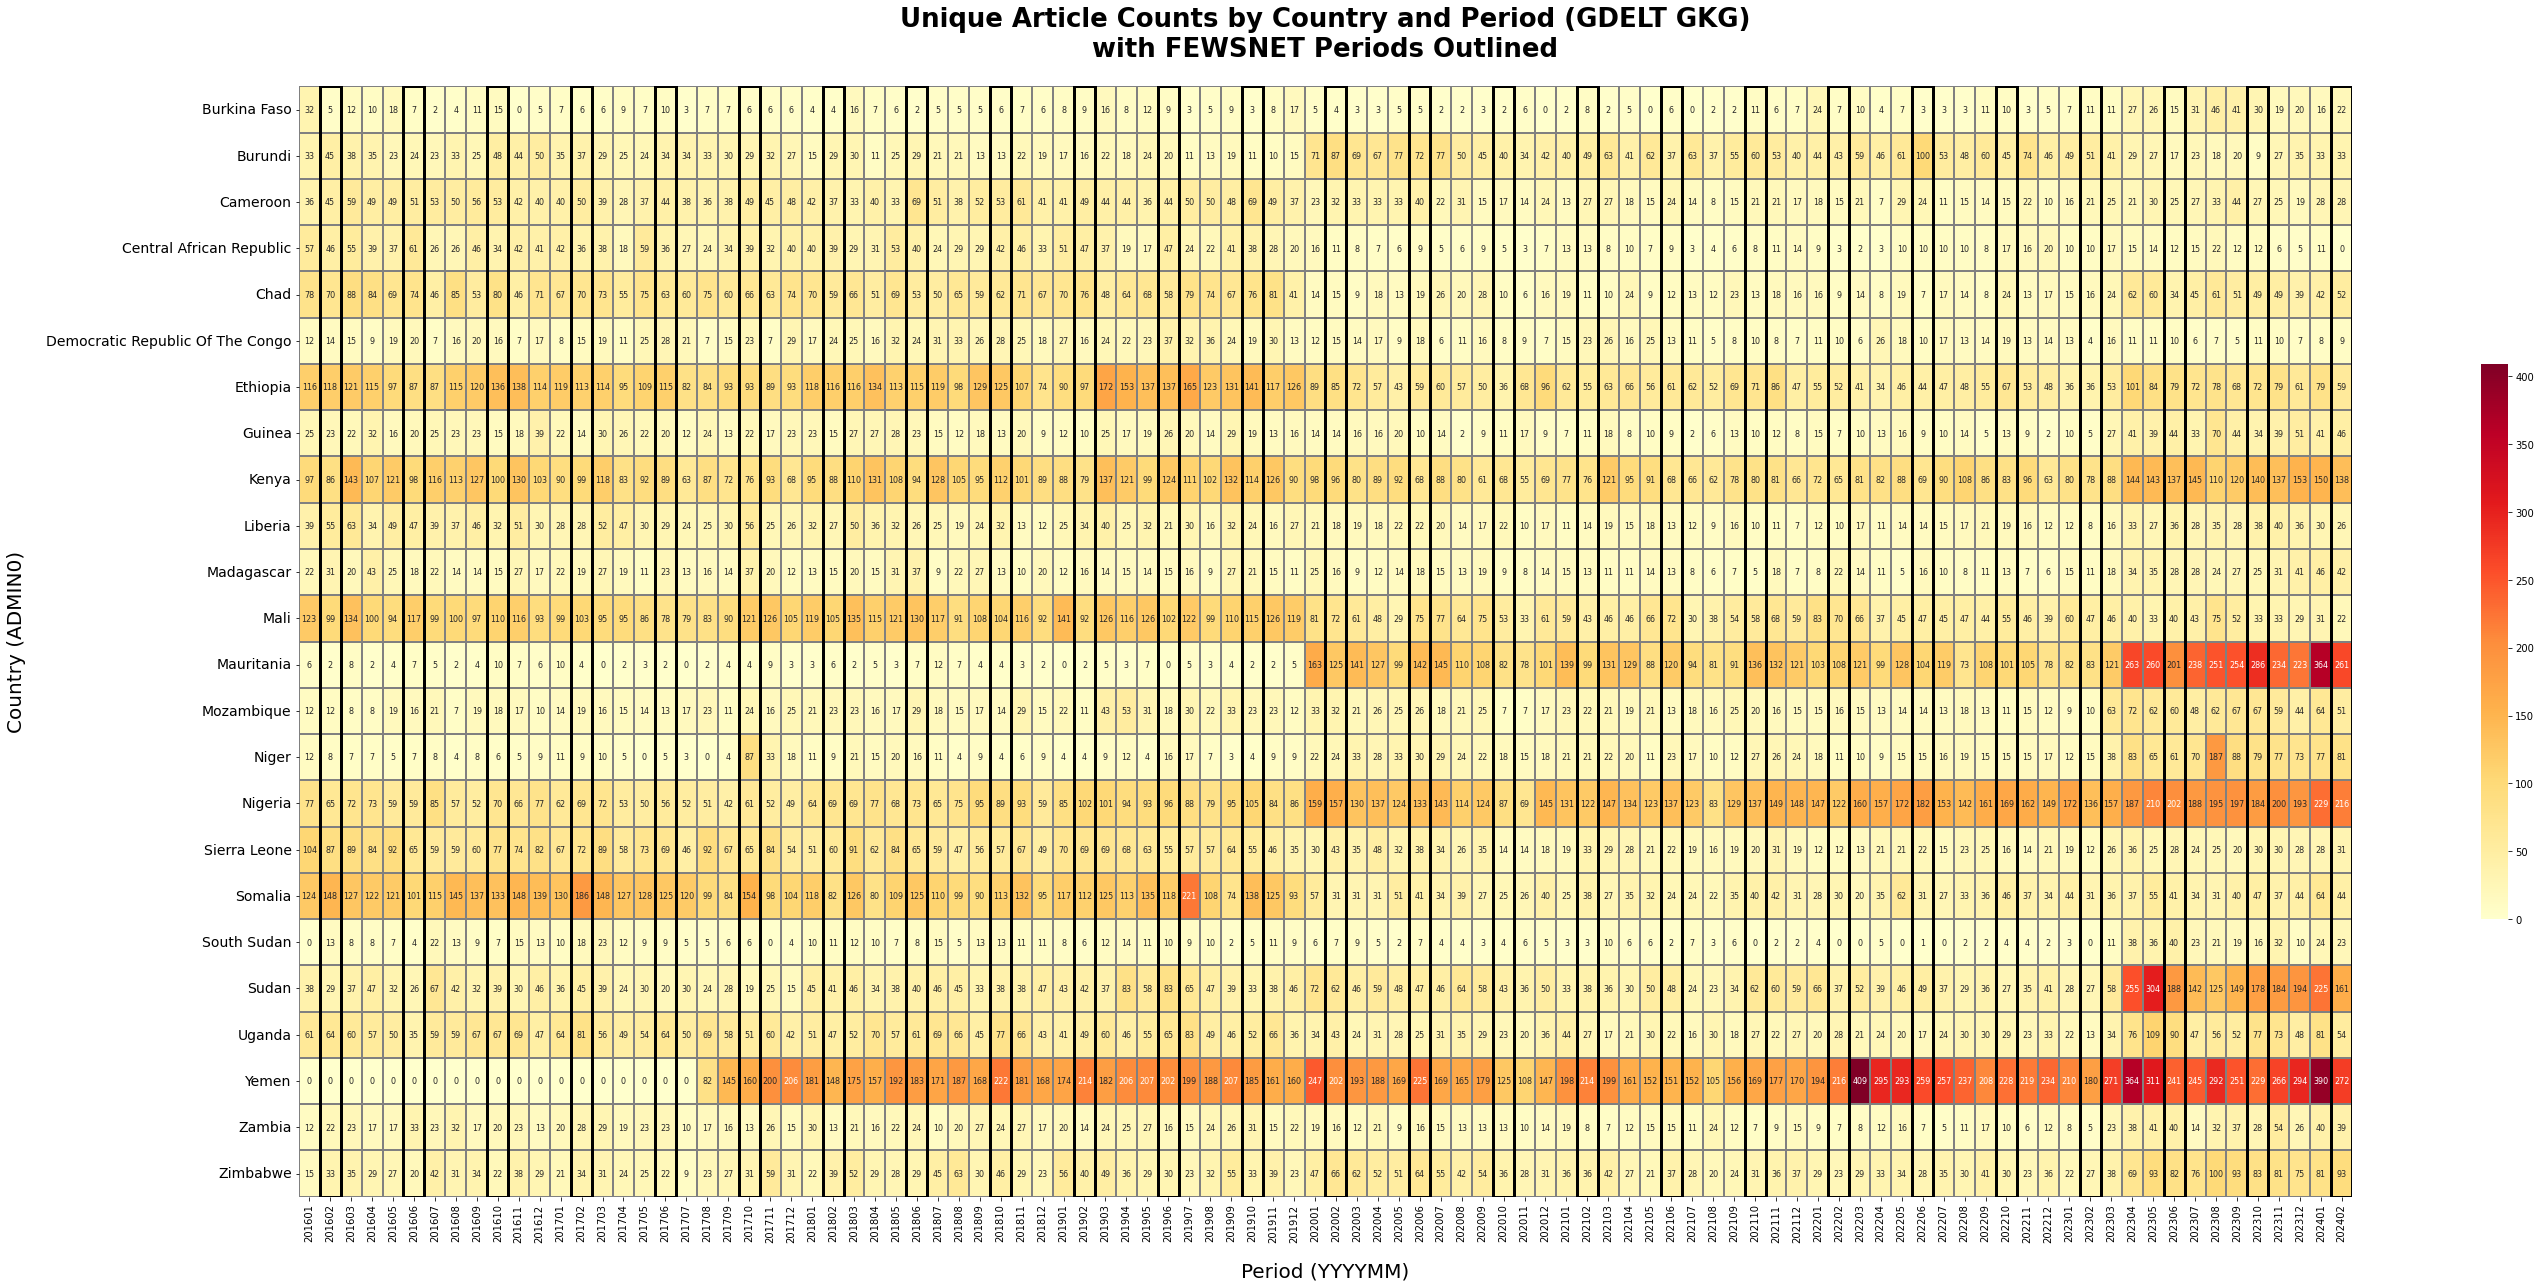
\includegraphics[width=1\textwidth]{gkg_article_counts.png}

\caption{Geographic and temporal distribution of GDELT article coverage across Africa and Yemen. 
\textbf{Top:} GDELT Events article counts. 
\textbf{Bottom:} GDELT GKG article counts. 
}
\label{fig:gdelt_temporal}
\end{figure}

\FloatBarrier
To contextualize these media coverage patterns against actual food security outcomes, we aggregated Integrated Phase Classification (IPC) scores by country and period (Figure~\ref{fig:ipc_mean}). This heatmap summarizes the mean IPC phase for each country and FEWS NET reporting round, providing a high-level view of food insecurity severity across the continent over time. Higher values indicate greater population exposure to crisis (Phase 3), emergency (Phase 4), or famine (Phase 5) conditions, while lower values reflect predominantly minimal (Phase 1) or stressed (Phase 2) food security environments. Comparing these trends to the media signal maps enables a direct visual assessment of the correspondence between humanitarian need and media attention.

\begin{figure}[H]
    \centering
    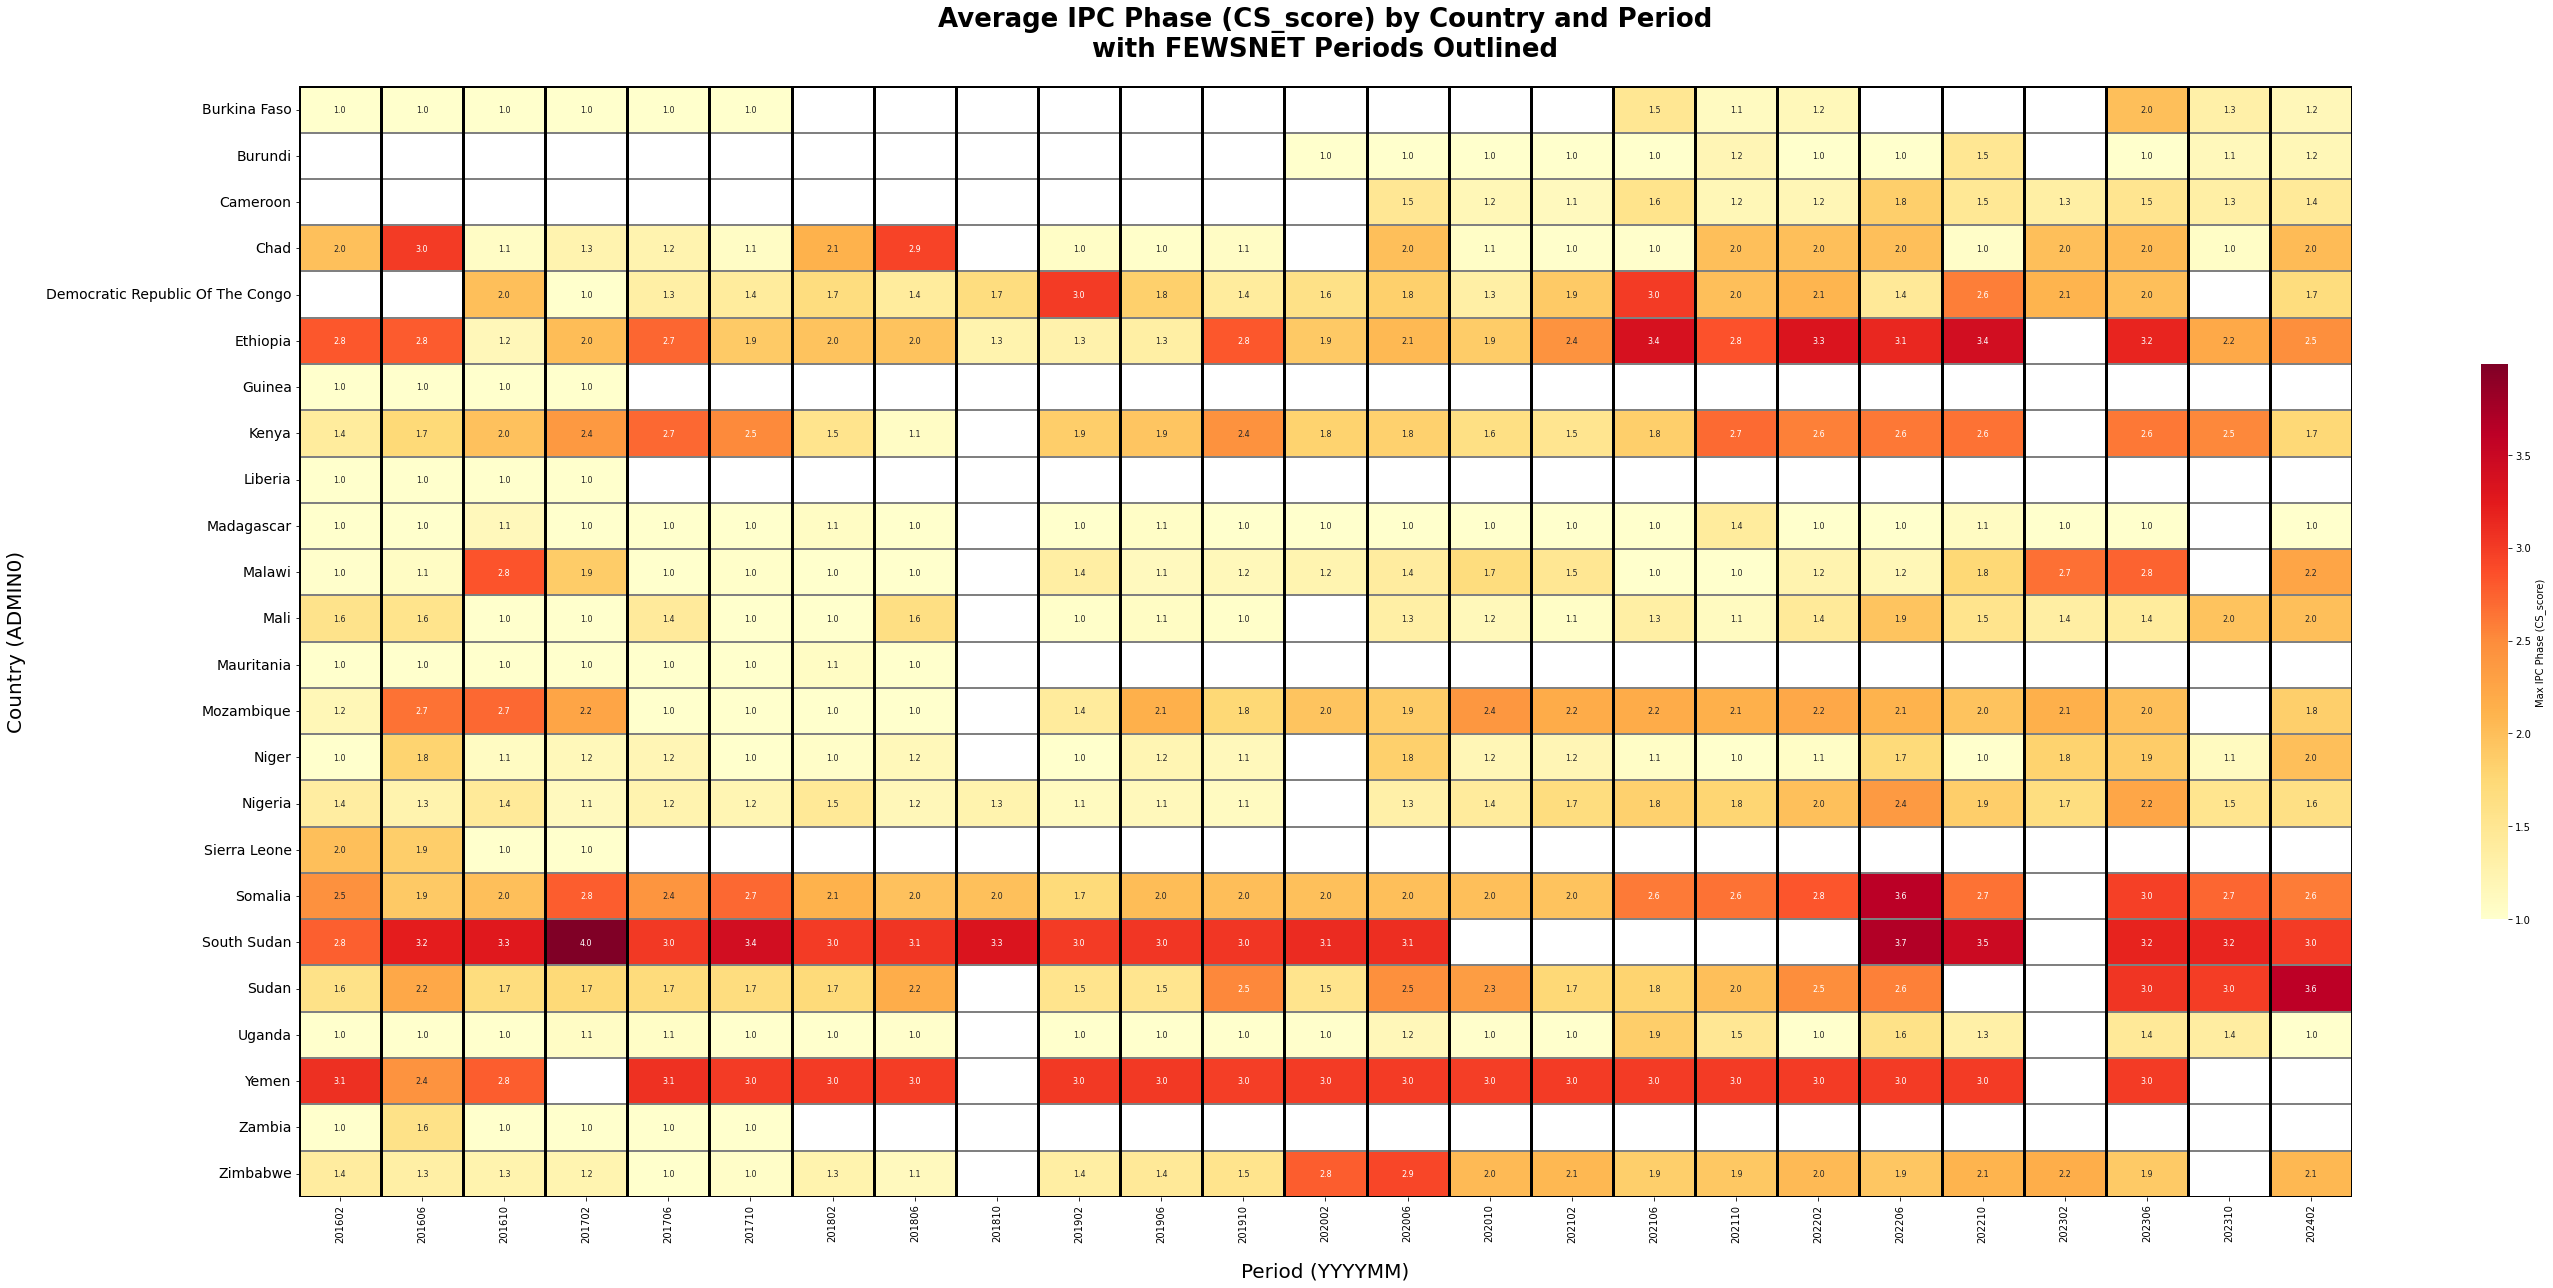
\includegraphics[width=1\textwidth]{mean_ipc.png}
    \caption{
        \textbf{Country-level mean IPC phase by FEWS NET period (2016--2024).}
        Each cell shows the arithmetic mean of the highest reported IPC phase across all administrative units within a country and FEWS NET reporting round. 
        Values closer to 1 indicate minimal food insecurity; values of 3 or higher correspond to widespread crisis, emergency, or famine conditions. 
        Bold outlines denote official FEWS NET analysis periods.
    }
    \label{fig:ipc_mean}
\end{figure}


Since our objective is to evaluate the feasibility of using GDELT-derived signals for food security prediction, it is essential to assess data coverage at sub-national levels. To this end, we examined the distribution of article counts across predefined buckets at the ADMIN1 (Figure~\ref{fig:admin1_distributions}) and ADMIN2 (Figure~\ref{fig:admin2_distributions}) spatial scales. \\

The resulting distributions reveal stark contrasts between the two GDELT products. The Events dataset exhibits relatively broad coverage at both administrative levels, with a substantial share of regions and districts falling into non-zero article-count buckets. Even at the ADMIN2 level, a meaningful number of districts receive between 1 and 50 articles, and a non-negligible fraction exceed 50 articles, indicating geographically widespread event reporting. \\

By contrast, the GKG dataset displays a highly concentrated and zero-inflated distribution. Already at the ADMIN1 level, the vast majority of regions receive no GKG articles at all, while a small number of regions accumulate very high article counts. This imbalance becomes even more pronounced at the ADMIN2 level, where only a tiny fraction of districts fall into the highest coverage bucket (50+ articles), and the overwhelming majority receive zero coverage. The resulting long-tailed distribution indicates that GKG-derived signals are heavily driven by a limited set of highly visible locations. \\

These patterns highlight a fundamental trade-off between the two data sources. While GKG provides rich narrative and thematic information where coverage exists, its severe spatial sparsity at fine geographic scales poses challenges for comprehensive sub-national modelling. In contrast, the Events dataset offers broader and more evenly distributed spatial coverage, making it better suited as a baseline signal for district-level prediction tasks. \\

Based on this evidence of severe spatial sparsity, we excluded GKG-derived features from the predictive models presented in subsequent sections, relying exclusively on GDELT Events features for downstream prediction tasks.

\begin{figure}[H]
    \centering

    % Top: Events (ADMIN1)
    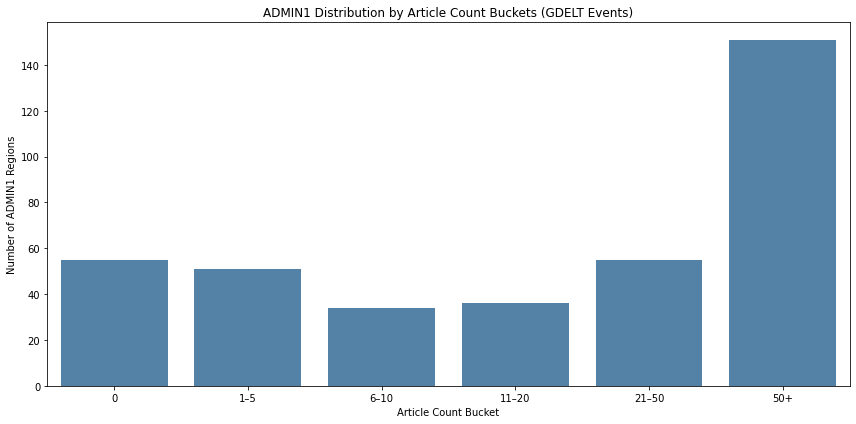
\includegraphics[width=0.5\textwidth]{admin1_distribution.png}

    \vspace{0.5em}

    % Bottom: GKG (ADMIN1)
    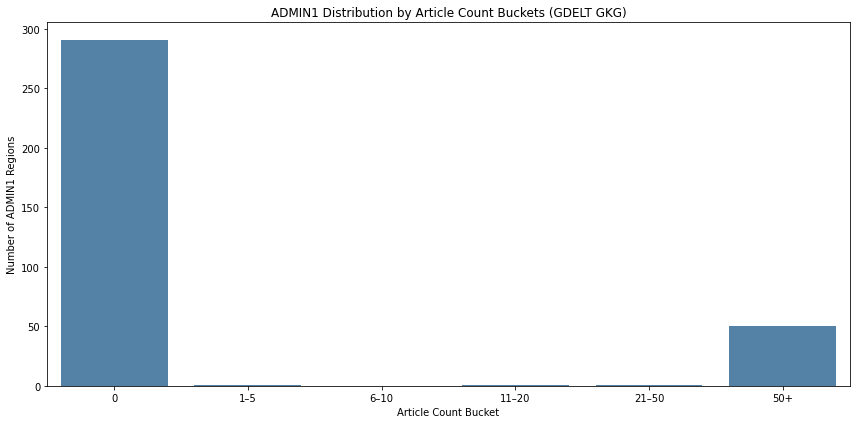
\includegraphics[width=0.5\textwidth]{gkg_admin1_distribution.png}

    \caption{Distribution of article counts at the ADMIN1 level across GDELT data sources.
    \textbf{Top:} GDELT Events, showing a relatively broad spread across multiple article-count buckets.
    \textbf{Bottom:} GDELT Global Knowledge Graph (GKG), exhibiting a highly concentrated and zero-inflated distribution, with most regions receiving no coverage and a small number accumulating very high counts.}
    \label{fig:admin1_distributions}
\end{figure}

\begin{figure}[H]
    \centering

    % Top: Events (ADMIN2)
    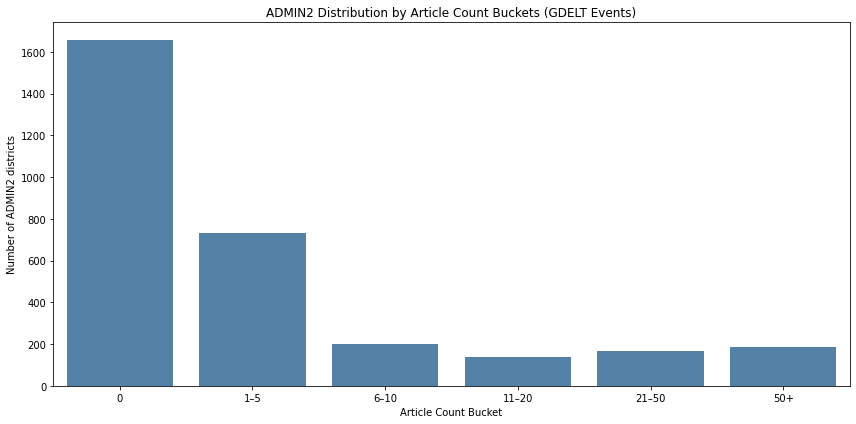
\includegraphics[width=0.5\textwidth]{admin2_distribution.png}

    \vspace{0.5em}

    % Bottom: GKG (ADMIN2)
    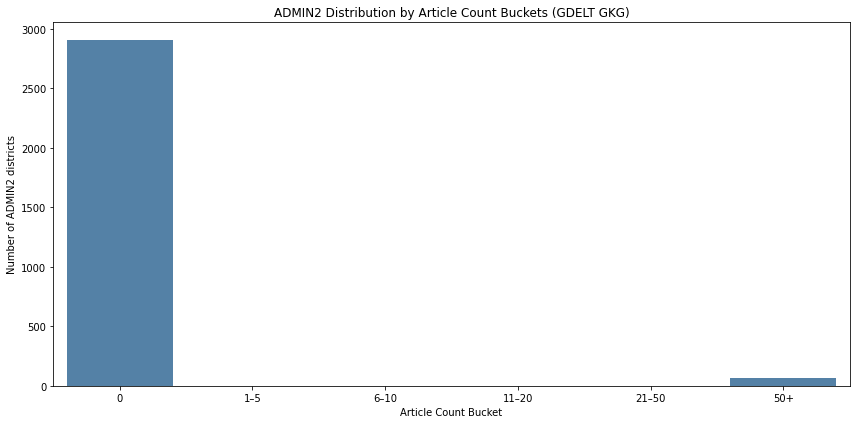
\includegraphics[width=0.5\textwidth]{gkg_admin2_distribution.png}

    \caption{Distribution of article counts at the ADMIN2 level across GDELT data sources.
    \textbf{Top:} GDELT Events, showing a meaningful spread across districts, with many ADMIN2 units receiving non-zero coverage across multiple count buckets.
    \textbf{Bottom:} GDELT Global Knowledge Graph (GKG), exhibiting extreme sparsity at this spatial scale: the vast majority of districts receive zero articles, while only a very small number accumulate high article counts.}
    \label{fig:admin2_distributions}
\end{figure}

\FloatBarrier

To assess whether variation in media coverage systematically co-varies with observed food security conditions, we conduct a diagnostic regression analysis relating article volumes to contemporaneous FEWS NET food security classifications. Specifically, we estimate an ordinary least squares model with country and period fixed effects, regressing the number of articles published between successive FEWS NET reporting periods on the corresponding IPC-based food security score. This analysis is not intended to establish causality, but rather to evaluate whether each GDELT product exhibits a systematic association with observed food security conditions after controlling for time-invariant country characteristics and common temporal shocks. \\

For the Events dataset, we find a positive and statistically significant association between food security severity and article volume. Specifically, a one-phase increase in the IPC CS score is associated with an average increase of approximately 33 event-based articles between reporting periods ($p < 0.01$). This pattern is broadly consistent with the descriptive distributions shown in Figure~\ref{fig:appendix_raw_scatter}, where higher IPC phases tend to correspond to somewhat higher densities of event reporting despite substantial dispersion across observations. \\

To assess whether this association reflects food-security-specific reporting rather than general country-month media attention, we benchmark FS-filtered article counts against total (unfiltered) GDELT country-month volume from the public \texttt{gdelt-bq.gdeltv2.events} feed. In proportional (log) terms FS-filtered news responds roughly twice as strongly to IPC severity as total news: $+12.6\%$ per IPC phase versus $+6.3\%$, with country and period fixed effects on $N=404$ country-months ($p<0.01$ vs $p\approx 0.05$; Figure~\ref{fig:appendix_log_scatter}). In raw levels the two counts are near-collinear at this aggregation (pairwise correlation $\approx 0.77$), so when entered jointly in a level fixed-effects regression neither is individually identified — a textbook collinearity outcome that is consistent with proportional responsiveness being the appropriate unit for highly skewed media data rather than evidence against the filter. We therefore interpret the keyword filter as amplifying news sensitivity to food security severity, particularly in low-baseline-coverage countries that level regressions implicitly downweight, while remaining linearly close to overall country-month media attention. \\

In contrast, applying the same specification to the GKG dataset yields no statistically significant relationship between article counts and IPC CS scores. This divergence is consistent with earlier spatial and temporal diagnostics: while event-based reporting tends to spike around discrete shocks that often co-occur with acute food security deterioration, GKG coverage reflects broader narrative attention that evolves more gradually and appears less sensitive to marginal changes in IPC phase. Taken together, these results suggest that event-based media signals exhibit more concentrated short-run co-movement with food security dynamics, whereas GKG-derived measures appear to capture complementary but less temporally responsive dimensions of information. Combined with the spatial sparsity documented above, these patterns motivated our decision to exclude GKG-derived features from the predictive models and to rely on GDELT Events features for downstream food security prediction. \\

To support this interpretation and provide greater transparency on the structure of the underlying media signals, we include a comprehensive set of diagnostic heatmaps in the Appendix (Supplementary Figures~S5--S27). These figures visualise the country-by-period distribution of key features extracted from both GDELT Events and GKG data, including conflict- and crisis-related indicators and predicted humanitarian resource needs. Consistent with the regression results, the Events-based heatmaps display sparse but sharply defined temporal spikes aligned with discrete shocks, whereas GKG-derived heatmaps exhibit smoother and more persistent patterns reflecting sustained narrative coverage. These diagnostics are not used directly for inference, but serve to validate feature construction choices and to illustrate the heterogeneous and non-random nature of media-derived signals used in subsequent predictive analyses. \\

To verify directly that the contemporaneous co-movement above translates into forward-looking content, we run a complementary lead-lag panel regression in which today's FS-filtered article volume predicts the IPC CS score at the $k$th next observed assessment ($k=1,\dots,4$), with country and period fixed effects (Table~\ref{tab:lead_lag_diagnostic}). Conditional on today's IPC, today's article volume remains significantly associated with future IPC at $k=1$ ($p=0.005$) and $k=2$ ($p=0.021$) -- the same horizons as the predictive analyses in Section~\ref{sec:modelling_results} -- loses significance at $k=3$ ($p=0.159$), and is again marginally significant at $k=4$ ($p=0.085$). At $k=4$, however, today's IPC itself is no longer statistically distinguishable from zero ($\hat\beta=0.030$, $p=0.586$), so GDELT is the only marginally informative predictor at the longest horizon. The lead-lag panel therefore provides direct evidence that GDELT carries forward-looking food-security information beyond IPC persistence at the one- to two-assessment-ahead horizon, complementing the contemporaneous and proportional findings above. \\

\paragraph{Limitations and scope.}
Several limitations of news-derived media data should be noted before turning to predictive modelling. First, media coverage is uneven across space and time, reflecting journalistic priorities, language availability, and geopolitical salience rather than a uniform sampling of on-the-ground conditions. As shown in the preceding diagnostics, this results in substantial spatial sparsity at fine administrative levels, particularly for narrative-rich sources such as the GDELT Global Knowledge Graph, which may constrain model performance in low-coverage regions. Second, media reports may respond endogenously to severe or highly visible crises, raising the possibility that some signals capture contemporaneous attention rather than early warning. We address this concern by construction: the predictive analyses in Section~\ref{sec:modelling_results} use GDELT features observed strictly before each target IPC assessment, with forecast horizons of one and two reporting periods (approximately four and eight months) ahead, so any out-of-sample predictive lift in those models reflects information available at the time of the prediction rather than contemporaneous reporting of the target assessment itself. Third, the FEWS NET IPC classifications used as outcome variables are expert assessments rather than direct measurements, and therefore embed both judgement and information constraints. The analyses in this section are intended to characterise these structural properties and delimit the conditions under which news-derived signals are informative. The modelling results that follow should therefore be interpreted as conditional on these constraints, rather than as evidence of universal predictive capacity.

\subsection{Modelling Acute Food Insecurity from Text-Extracted Features}
\label{sec:modelling_results}

Having established the diagnostic properties of GDELT-derived signals in the preceding sections, we now evaluate their predictive value for food security modelling. We assess three prediction tasks of increasing difficulty: (i)~predicting the next IPC assessment level, (ii)~predicting IPC levels two assessment periods ahead (~8 months), and (iii)~predicting binary worsening transitions between consecutive assessments. For each task, we compare feature sets systematically to isolate the contribution of news-derived signals.

An important framing consideration guides interpretation throughout. Given the strong temporal autocorrelation of IPC scores, lagged IPC already captures much of the predictive signal. As a result, improvements over IPC-based baselines are inherently limited. The primary contribution of news-derived signals is therefore not to outperform IPC, but to provide a complementary or substitute signal when IPC assessments are unavailable, sparse, or delayed.

\subsubsection{Experimental Setup}

We train three classifiers, Logistic Regression (LR), Random Forest (RF), and CatBoost, on four primary feature sets: (1)~\textit{IPC only}, using only the most recent IPC score (forward-filled) and geographic dummy variables (one-hot encoding of ADMIN0, ADMIN1, and ADMIN2 identifiers, yielding 3{,}331 binary features that jointly capture country, region, and district context); (2)~\textit{IPC + GDELT base}, adding 119 aggregated GDELT Events features---comprising event and article counts, sentiment scores (mean, sum, count), named entity recognition frequencies at each administrative level, BERT-predicted impact/urgency/resource distributions, and crisis keyword indicators (fatalities, displacement, food insecurity, economic shocks); (3)~\textit{IPC + GDELT + temporal}, further adding 35 temporal features (rolling means over 3 and 6 periods, lags, and escalation indicators); and (4)~\textit{GDELT only}, using all GDELT features with geographic dummies but no lagged IPC score. We also evaluate variants without geographic dummies to assess the role of location context.

Evaluation follows a rolling temporal window protocol: for each IPC assessment period, models are trained on the preceding 20 monthly periods and tested on the held-out assessment. The 20-month window balances sufficient training data for stable estimation against responsiveness to distributional shifts in both media coverage and food security dynamics. This mimics a realistic operational forecasting scenario and avoids look-ahead bias. We report accuracy and macro-averaged F1 scores. Results are presented for two temporal scopes: the full evaluation window (25 assessment periods, 2016--2024) and a recent subset (last 6 assessment periods, 2022--2024), motivated by documented improvements in GDELT's geographic coverage and linguistic processing over time \citep{leetaru2013gdelt}.

\subsubsection{Task 1: Predicting the Next IPC Assessment}

Table~\ref{tab:next_ipc} presents results for predicting the next observed IPC phase (1--5). Logistic Regression consistently outperforms tree-based models across all feature sets, likely due to implicit regularisation in the high-dimensional feature space (3,300+ geographic dummies).

\begin{table}[H]
\centering
\small
\caption{Next IPC assessment prediction (macro-averaged). Best ML result per column in bold. Heuristic baselines are evaluated over 24 periods (one fewer than ML models) because they require at least one prior assessment to generate a prediction.}
\label{tab:next_ipc}
\begin{tabular}{ll cccc}
\toprule
& & \multicolumn{2}{c}{All periods (25)} & \multicolumn{2}{c}{Last 6 periods} \\
\cmidrule(lr){3-4} \cmidrule(lr){5-6}
Model & Feature Set & Acc & F1 & Acc & F1 \\
\midrule
\multicolumn{6}{l}{\textit{Heuristic baselines}} \\
PPS & -- & 0.708 & 0.727 & 0.613 & 0.640 \\
SPLY & -- & 0.676 & 0.695 & 0.649 & 0.674 \\
Max-2PP & -- & 0.731 & 0.738 & 0.671 & 0.679 \\
\midrule
\multicolumn{6}{l}{\textit{ML classifiers}} \\
LR & IPC only (CHS) & \textbf{0.838} & \textbf{0.836} & 0.773 & 0.775 \\
LR & IPC + GDELT base & 0.835 & 0.833 & 0.773 & 0.775 \\
LR & IPC + GDELT + temporal & 0.834 & 0.833 & 0.775 & 0.777 \\
LR & GDELT only & 0.837 & 0.834 & \textbf{0.793} & \textbf{0.794} \\
CatBoost & IPC only (CHS) & 0.740 & 0.738 & 0.638 & 0.635 \\
CatBoost & IPC + GDELT + temporal & 0.740 & 0.738 & 0.635 & 0.632 \\
RF & IPC only (CHS) & 0.735 & 0.740 & 0.649 & 0.650 \\
RF & IPC + GDELT base & 0.741 & 0.739 & 0.680 & 0.680 \\
LR & GDELT only (no geo) & 0.498 & 0.387 & 0.412 & 0.333 \\
\bottomrule
\end{tabular}
\end{table}

Two findings emerge. First, over the full evaluation window, GDELT-only features with geographic context achieve performance essentially equivalent to lagged IPC scores (F1 0.834 vs 0.836), demonstrating that news-derived signals can \textit{substitute} for lagged IPC scores where assessments are unavailable, delayed, or have coverage gaps. Second, when restricting evaluation to recent periods (2022--2024), GDELT-only shows a small edge over IPC-only of +0.020 F1 points (0.794 vs 0.775). This recent-period gain is consistent with the documented expansion of GDELT's geographic and linguistic coverage over time, but should be interpreted cautiously: the 2022--2024 window also coincides with several large geopolitical shocks (the Sudan civil war, Ukraine-related supply disruptions, post-COVID inflation) that disproportionately drive media volume and may inflate the apparent advantage. Geographic dummy variables are essential: without them, GDELT-only performance collapses to F1~0.333, indicating that news signals encode \textit{what is happening} but require location context to map to absolute IPC levels.

\subsubsection{Task 2: Longer-Horizon Forecasting (2 Assessments Ahead)}

To test whether GDELT features provide greater value at longer forecast horizons---where the most recent IPC score becomes increasingly stale---we predict IPC levels two assessment periods ahead (approximately 8 months). The target variable is constructed by looking forward two observed IPC assessments from each prediction point. Results are reported in Table~\ref{tab:longer_horizon}.

\begin{table}[H]
\centering
\small
\caption{Two-assessment-ahead IPC forecast (macro-averaged). Best ML result per column in bold. Heuristic baselines are evaluated over 22 periods (one fewer than ML models).}
\label{tab:longer_horizon}
\begin{tabular}{ll cccc}
\toprule
& & \multicolumn{2}{c}{All periods (23)} & \multicolumn{2}{c}{Last 6 periods} \\
\cmidrule(lr){3-4} \cmidrule(lr){5-6}
Model & Feature Set & Acc & F1 & Acc & F1 \\
\midrule
\multicolumn{6}{l}{\textit{Heuristic baselines}} \\
PPS & -- & 0.727 & 0.725 & 0.670 & 0.670 \\
SPLY & -- & 0.686 & 0.700 & 0.665 & 0.682 \\
Max-2PP & -- & 0.735 & 0.737 & 0.702 & 0.704 \\
\midrule
\multicolumn{6}{l}{\textit{ML classifiers}} \\
LR & GDELT only & \textbf{0.751} & \textbf{0.746} & \textbf{0.703} & \textbf{0.703} \\
LR & IPC only (CHS) & 0.746 & 0.740 & 0.703 & 0.703 \\
LR & IPC + GDELT base & 0.744 & 0.738 & 0.700 & 0.700 \\
LR & IPC + GDELT + temporal & 0.742 & 0.737 & 0.699 & 0.700 \\
CatBoost & IPC + GDELT + temporal & 0.719 & 0.721 & 0.657 & 0.660 \\
CatBoost & IPC only (CHS) & 0.717 & 0.719 & 0.658 & 0.662 \\
RF & IPC only (CHS) & 0.671 & 0.672 & 0.577 & 0.568 \\
\bottomrule
\end{tabular}
\end{table}

At the two-assessment horizon, GDELT-only outperforms IPC-only across the full evaluation window (F1 0.746 vs 0.740), confirming that as the lagged IPC score becomes stale, near-real-time news signals provide incrementally more useful information about current conditions. Over the most recent 6 periods, the two feature sets converge (both at F1~0.703). These results support the theoretical motivation for incorporating streaming media data into food security monitoring: at horizons beyond the most recent assessment, the informational advantage of expert classifications diminishes, and continuously updated news signals become relatively more valuable.

\subsubsection{Task 3: Transition Prediction}

We also evaluated a binary formulation: predicting whether an area's IPC score \textit{worsens} relative to the previous assessment (positive class $\approx$~12--17\% of observations). This task strips out the autocorrelation that dominates level prediction and directly tests whether models can detect escalation.

\begin{table}[H]
\centering
\small
\caption{Transition prediction---detecting IPC worsening (F1 for worsened class). Best ML result per column in bold. Heuristic baselines are evaluated over 24 periods (one fewer than ML models).}
\label{tab:transitions}
\begin{tabular}{ll cccc}
\toprule
& & \multicolumn{2}{c}{All periods (25)} & \multicolumn{2}{c}{Last 6 periods} \\
\cmidrule(lr){3-4} \cmidrule(lr){5-6}
Model & Feature Set & Acc & F1 & Acc & F1 \\
\midrule
\multicolumn{6}{l}{\textit{Heuristic baselines}} \\
No-Change & -- & 0.874 & 0.000 & 0.829 & 0.000 \\
Always-Worsen & -- & 0.126 & 0.216 & 0.171 & 0.279 \\
SPLY-Transition & -- & 0.829 & 0.185 & 0.776 & 0.215 \\
\midrule
\multicolumn{6}{l}{\textit{ML classifiers}} \\
LR & IPC only (CHS) & \textbf{0.914} & \textbf{0.718} & 0.893 & \textbf{0.705} \\
LR & IPC + GDELT base & 0.912 & 0.708 & 0.893 & 0.703 \\
LR & IPC + GDELT + temporal & 0.913 & 0.704 & \textbf{0.895} & 0.701 \\
LR & GDELT only & 0.711 & 0.445 & 0.630 & 0.437 \\
CatBoost & IPC + GDELT + temporal & 0.776 & 0.447 & 0.794 & 0.521 \\
CatBoost & IPC only (CHS) & 0.770 & 0.443 & 0.789 & 0.519 \\
RF & IPC + GDELT + temporal & 0.779 & 0.395 & 0.776 & 0.468 \\
RF & IPC only (CHS) & 0.686 & 0.376 & 0.686 & 0.426 \\
\bottomrule
\end{tabular}
\end{table}

Results are reported in Table~\ref{tab:transitions}. For transition prediction, the lagged IPC score dominates. Logistic Regression with IPC-only achieves the highest F1 (0.718) with near-perfect recall (99.5\%), and adding GDELT features slightly reduces performance. This result reflects the strong autocorrelation in food security dynamics: the most recent IPC score, combined with location fixed effects, already captures most of the information relevant to detecting worsening. Tree-based models (CatBoost, RF) show modest improvements from GDELT features in recent periods (+0.003 to +0.042 F1), suggesting that news signals may capture some escalation dynamics that linear models cannot exploit, though the overall gains remain small.

This negative finding is itself informative. It indicates that GDELT-derived features primarily encode information about \textit{absolute food security levels}---where a region sits on the IPC scale---rather than \textit{directional changes} in food security status. In other words, news coverage reflects the severity of a situation more than whether conditions are improving or deteriorating, a distinction that has implications for how media-derived signals should be deployed in operational monitoring systems.

\subsubsection{Summary of Predictive Findings}

Across all three prediction tasks, the results support three principal conclusions:

\begin{enumerate}
    \item \textbf{GDELT as IPC substitute.} When lagged IPC scores are unavailable, GDELT features combined with geographic context achieve comparable predictive performance for IPC level prediction (F1 0.834 vs.\ 0.836 over all periods), with a small recent-period edge of +0.020 F1 points (0.794 vs.\ 0.775; 2022--2024) that warrants caution given concurrent geopolitical shocks. This finding has direct operational relevance for regions with gaps in IPC assessment coverage, for monitoring between assessment cycles, and for rapid deployment in newly affected areas.

    \item \textbf{Increasing value at longer horizons.} At two-assessment-ahead forecasting, GDELT-only outperforms IPC-only even over the full evaluation window, confirming that continuously updated news signals become relatively more informative as lagged IPC scores become stale. This supports the use of news-derived features in medium-term monitoring applications.

    \item \textbf{Geographic context is essential.} Without location fixed effects, all GDELT-based models collapse (F1~0.33--0.39), demonstrating that news signals must be interpreted within spatial context. This finding underscores the importance of geographically grounded feature engineering when using media data for food security prediction.
\end{enumerate}

The transition prediction results further clarify the nature of GDELT's informational content: news-derived features capture variation in food security \textit{levels} rather than \textit{changes}, suggesting they are best suited for nowcasting and level estimation rather than directional early warning. Taken together, these findings delineate both the promise and the boundaries of using open-source news data as an input to food security modelling.

\subsubsection{Feature Importance Analysis}

To understand which GDELT-derived signals drive predictive performance, we examined feature importance scores from the Random Forest models. Figure~\ref{fig:feature_importance} presents the top-ranked features for the next-IPC prediction task under two configurations: the full model (IPC + GDELT + temporal) and the GDELT-only model (no lagged IPC score).

\begin{figure}[H]
    \centering
    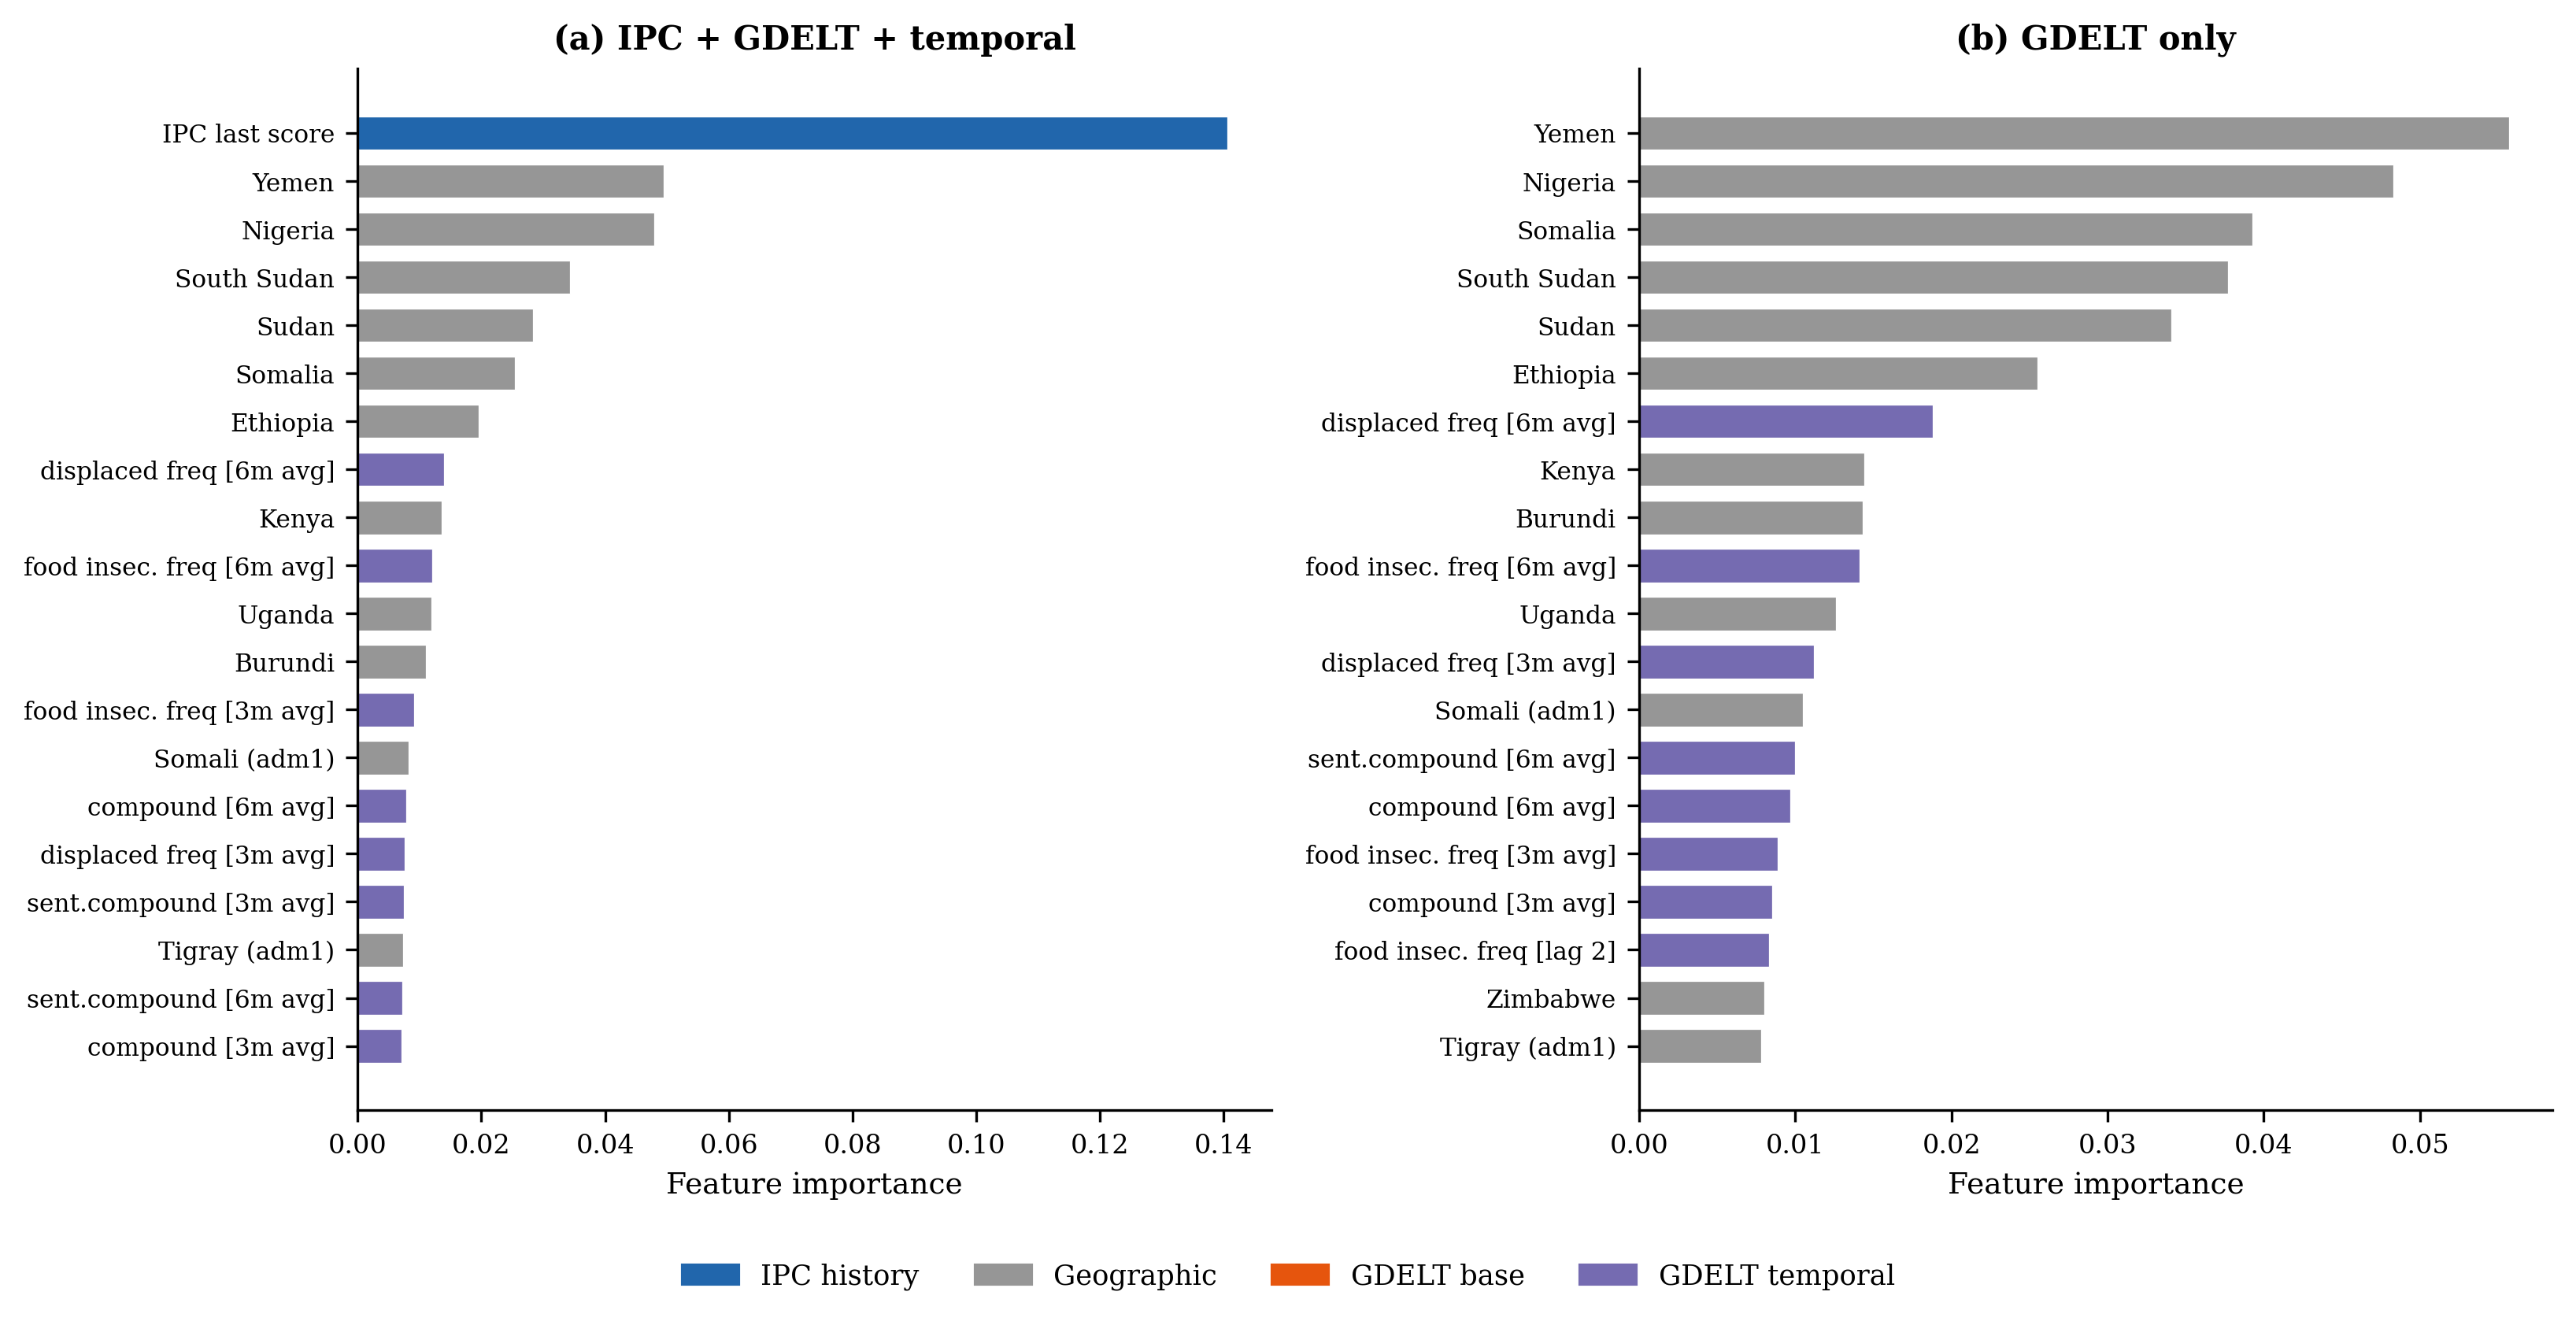
\includegraphics[width=\textwidth]{feature_importance.png}
    \caption{Top 20 features by importance (Random Forest, next-IPC prediction). \textbf{(a)}~Full model (IPC + GDELT + temporal): the most recent IPC score dominates, followed by country fixed effects; among GDELT features, displacement and food insecurity rolling averages rank highest. \textbf{(b)}~GDELT-only model: without lagged IPC scores, geographic context absorbs much of the importance, with temporal GDELT features---particularly displacement frequency and food insecurity frequency rolling averages---emerging as the leading news-derived signals. Feature categories are colour-coded: \textcolor[HTML]{2166ac}{IPC history}, \textcolor[HTML]{969696}{geographic}, \textcolor[HTML]{e6550d}{GDELT base}, \textcolor[HTML]{756bb1}{GDELT temporal}.}
    \label{fig:feature_importance}
\end{figure}

A natural concern is whether predictive performance is driven primarily by raw country-month news volume rather than by content-specific signal. Our feature aggregation step creates a per-period \texttt{\_count} feature for every list-typed input (e.g., \texttt{evt\_clean\_text\_count}, \texttt{evt\_NER\_count}, \texttt{evt\_compound\_score\_count}), each of which effectively records the number of articles contributing to a given country-period. None of these article-volume proxies appears among the top-25 most important features in any of the four configurations evaluated. The few \texttt{\_count}-named features that do rank (e.g., \texttt{evt\_displaced\_count\_mean},  \\ \texttt{evt\_fatalities\_count\_sum}) are NLP-extracted per-article counts of \emph{displaced persons} or \emph{fatalities}, not counts of articles. Predictive performance is therefore driven by content-extracted aggregations (displacement and food-insecurity frequencies, sentiment compound scores, BERT-derived resource indicators), the previous IPC score, and geographic dummies. We accordingly do not include total country-month news volume as a separate control: the random forest already has access to article-volume signal through the existing \texttt{\_count} features but does not assign it meaningful importance. \\

Notably, the BERT-derived features (predicted impact type, urgency, and resource need distributions) do not appear among the top-ranked individual features. Their contribution is instead distributed across multiple correlated indicators, each carrying modest individual importance. This suggests that while the MultiTaskBERT pipeline enriches the feature space, the dominant predictive signal comes from structured event counts and keyword-based indicators rather than from article-level NLP classifications. Isolating the marginal contribution of BERT features through ablation remains a direction for future work.

\subsubsection{Case Studies: GDELT Signals as Near-Real-Time Crisis Indicators}

To ground the statistical findings in operational context, we examine three crisis episodes where ADMIN2-level IPC scores deteriorated sharply. These cases are illustrative rather than representative: they were selected for crisis-type diversity (civil war, regional conflict, natural disaster) and sufficient GDELT coverage to permit meaningful signal inspection, and should not be taken as evidence of generalisable performance across all settings. Each case represents a distinct crisis driver and geographic setting, allowing us to assess whether GDELT-derived signals provided visible near-real-time indicators across heterogeneous scenarios. Figure panels show, from top to bottom: (i)~GDELT event counts overlaid with IPC phase assessments, (ii)~the subset of scraped articles from which NLP features were extracted, (iii)~reported fatality and displacement counts mentioned in articles, and (iv)~keyword frequencies for fatalities, displacement, food insecurity, and weather/climate. News-derived signals can relate to IPC classifications in three modes: \emph{leading} (e.g., displacement or market-price reporting that surfaces before the next FEWS NET assessment), \emph{coinciding} (e.g., active-conflict coverage that moves at the same pace as conditions on the ground), or \emph{following} (e.g., post-classification humanitarian-response coverage). The dominant mode varies with crisis type and IPC reporting cadence, and the three cases below illustrate this heterogeneity.

\paragraph{Sudan --- Khartoum (civil war).}
The Sudan civil war erupted on 15 April 2023 (Figure~\ref{fig:case_sudan}). Prior to the conflict, Khartoum was consistently assessed at IPC~1--2, with low GDELT coverage. Immediately following the war's onset, GDELT event counts surge from $\sim$500 to over 5{,}000 per month, scraped article counts increase tenfold, and fatality keyword mentions spike from near zero to over 700. Critically, a 12-month gap in IPC assessments (June 2022 to June 2023) means no official food security classification was available during the initial crisis escalation, precisely the period where GDELT signals were most active. When IPC assessments resumed in June 2023, Khartoum was classified at IPC~3, rising to IPC~4 by February 2024. This case illustrates the gap-filling potential suggested by the predictive analysis: where official assessments are delayed or disrupted, near-real-time news signals can help fill the monitoring gap.

\begin{figure}[H]
    \centering
    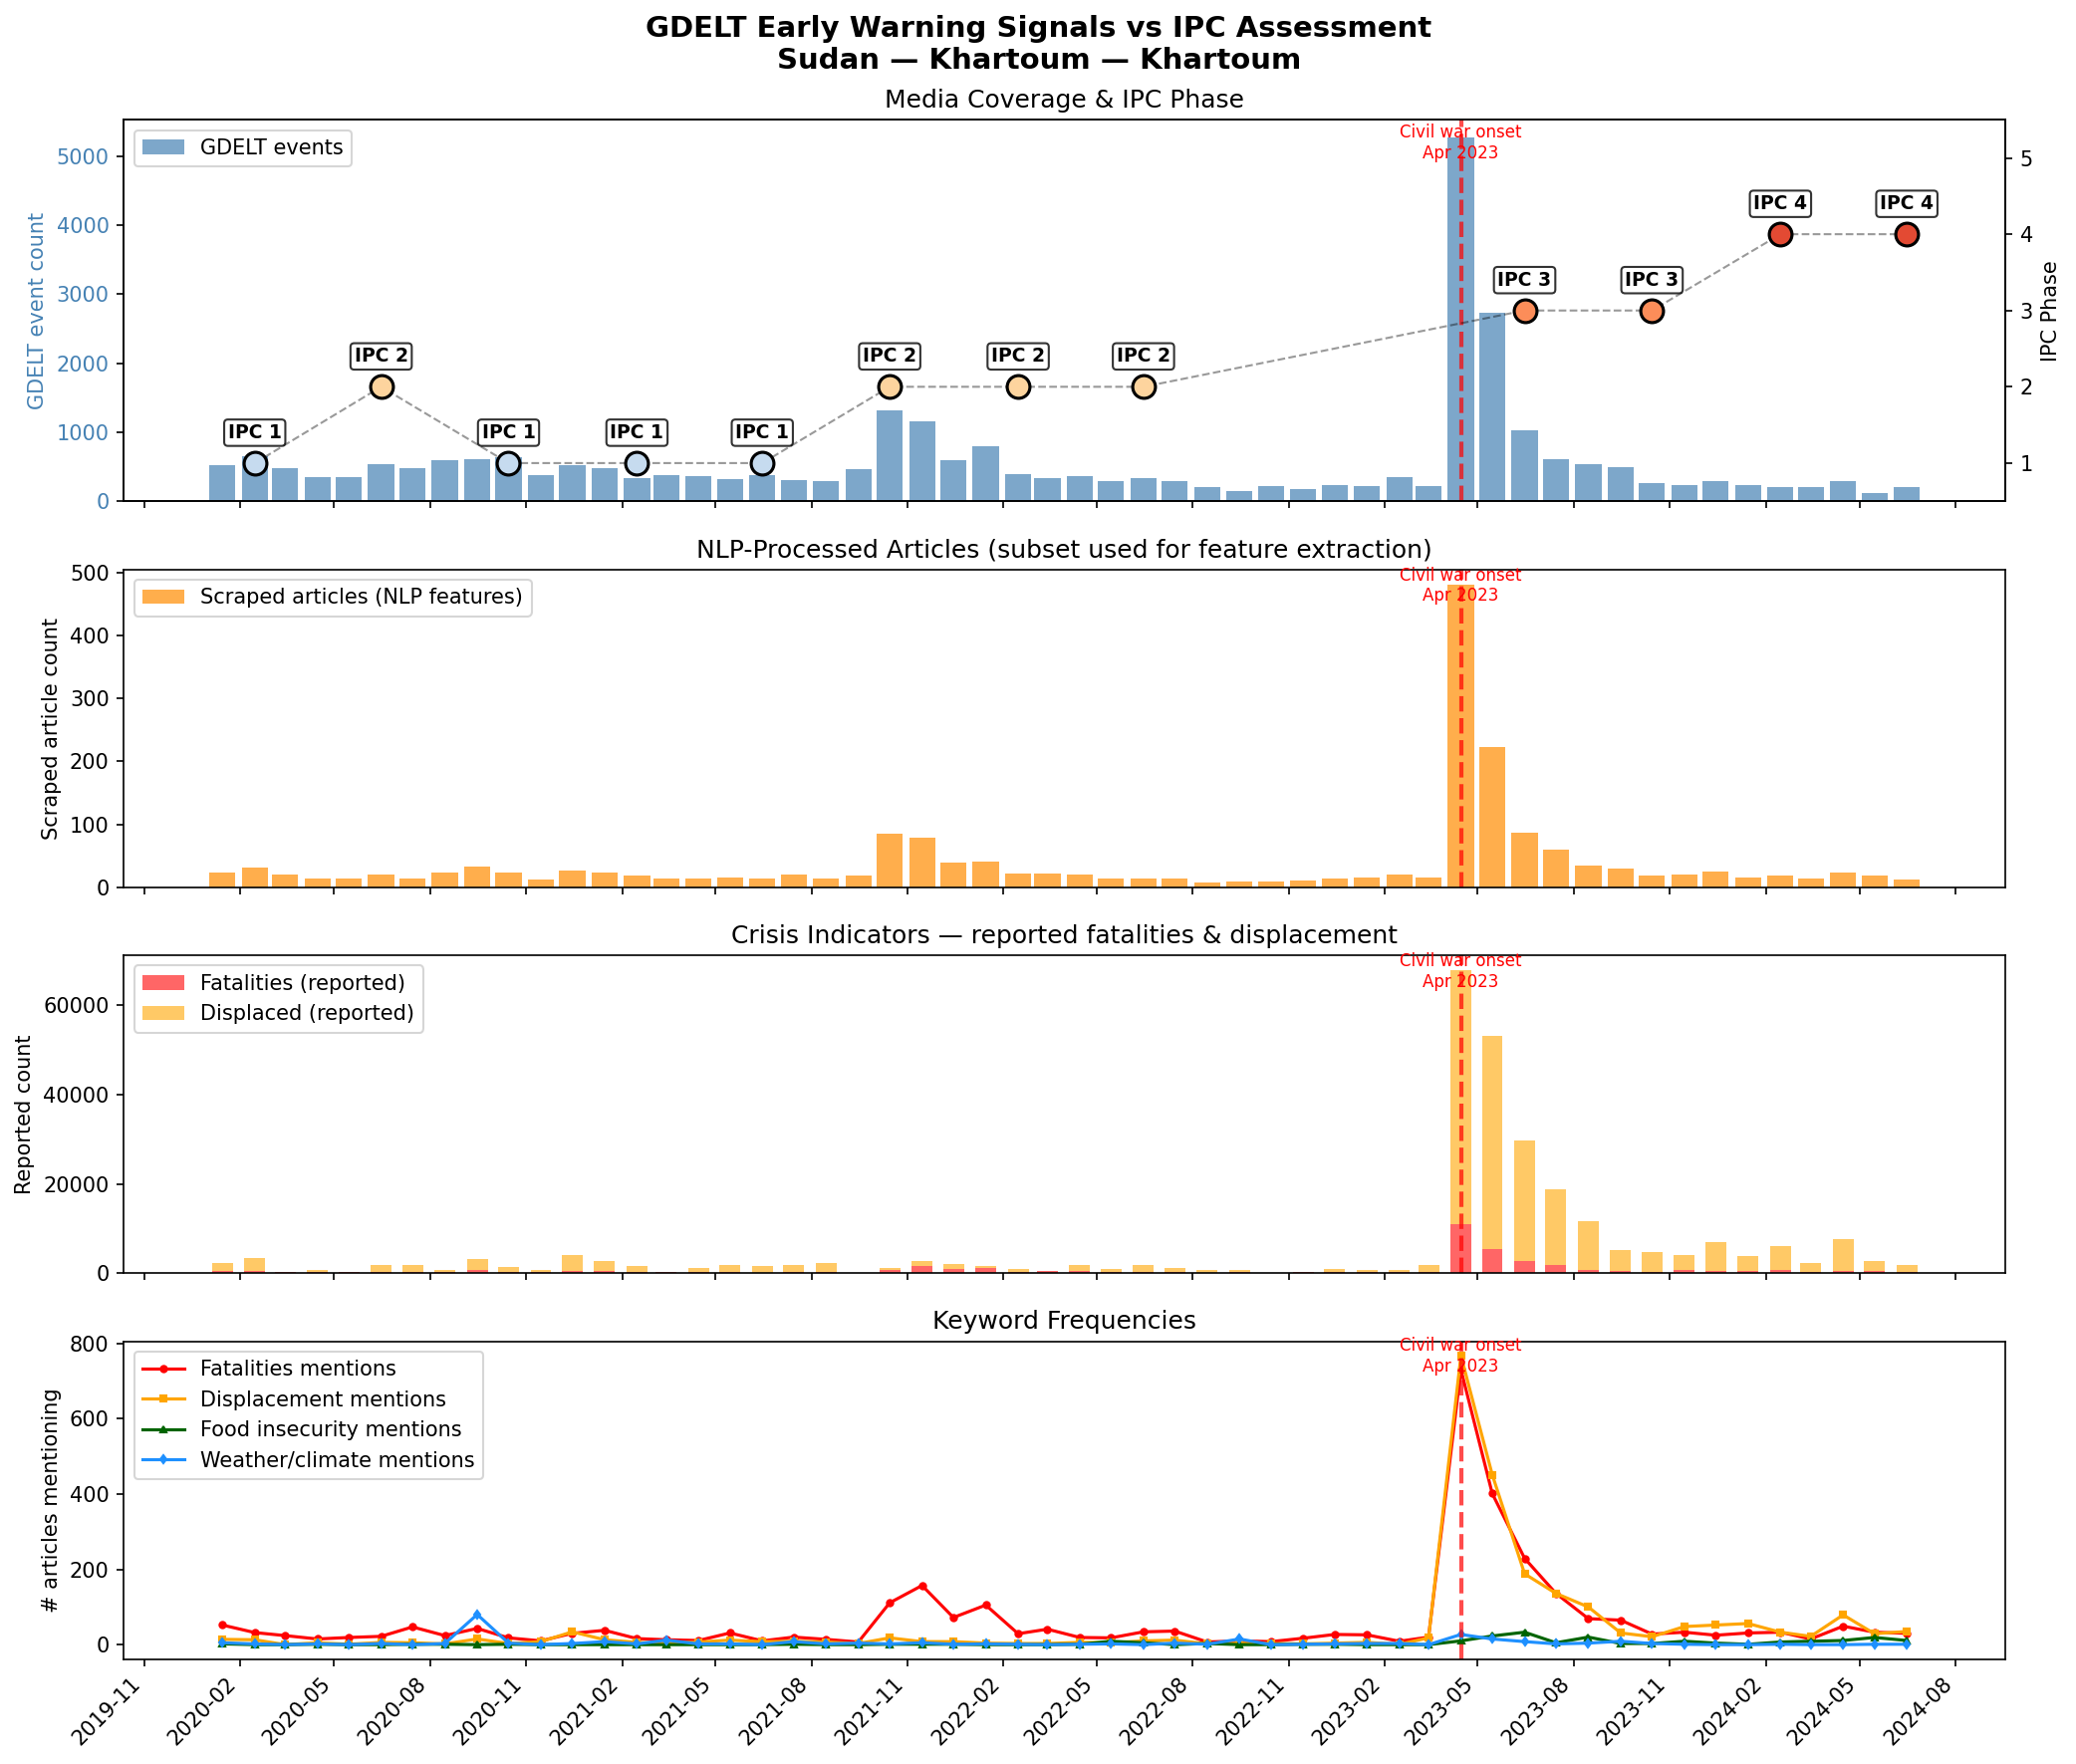
\includegraphics[width=\textwidth]{crisis_timeline_sudan_khartoum_khartoum.png}
    \caption{GDELT near-real-time media signals vs.\ IPC assessment timeline for Khartoum, Sudan. The vertical dashed line marks the onset of the civil war (April 2023). Note the 12-month gap in IPC assessments during the initial crisis period.}
    \label{fig:case_sudan}
\end{figure}

\paragraph{Ethiopia --- South Tigray (regional conflict).}
The Tigray conflict began on 4 November 2020 (Figure~\ref{fig:case_ethiopia}). South Tigray had been assessed at IPC~1--2 since 2019. GDELT event counts spike sharply at the war's onset, from $\sim$100 to nearly 1{,}800 per month, accompanied by a surge in scraped articles (from $<$10 to $>$130) and displacement counts exceeding 20{,}000. The IPC classification jumped from 2 to 4 in the February 2021 assessment, within months of the conflict's start, and remained at IPC~4 for the following three years. The keyword frequency panel shows fatality and displacement mentions dominating the signal, consistent with the conflict-driven nature of the crisis. Unlike the Sudan case, IPC assessments continued throughout the conflict, and the GDELT signal spike coincided with, rather than preceded, the IPC deterioration, reflecting the rapid pace of the Tigray crisis escalation.

\begin{figure}[H]
    \centering
    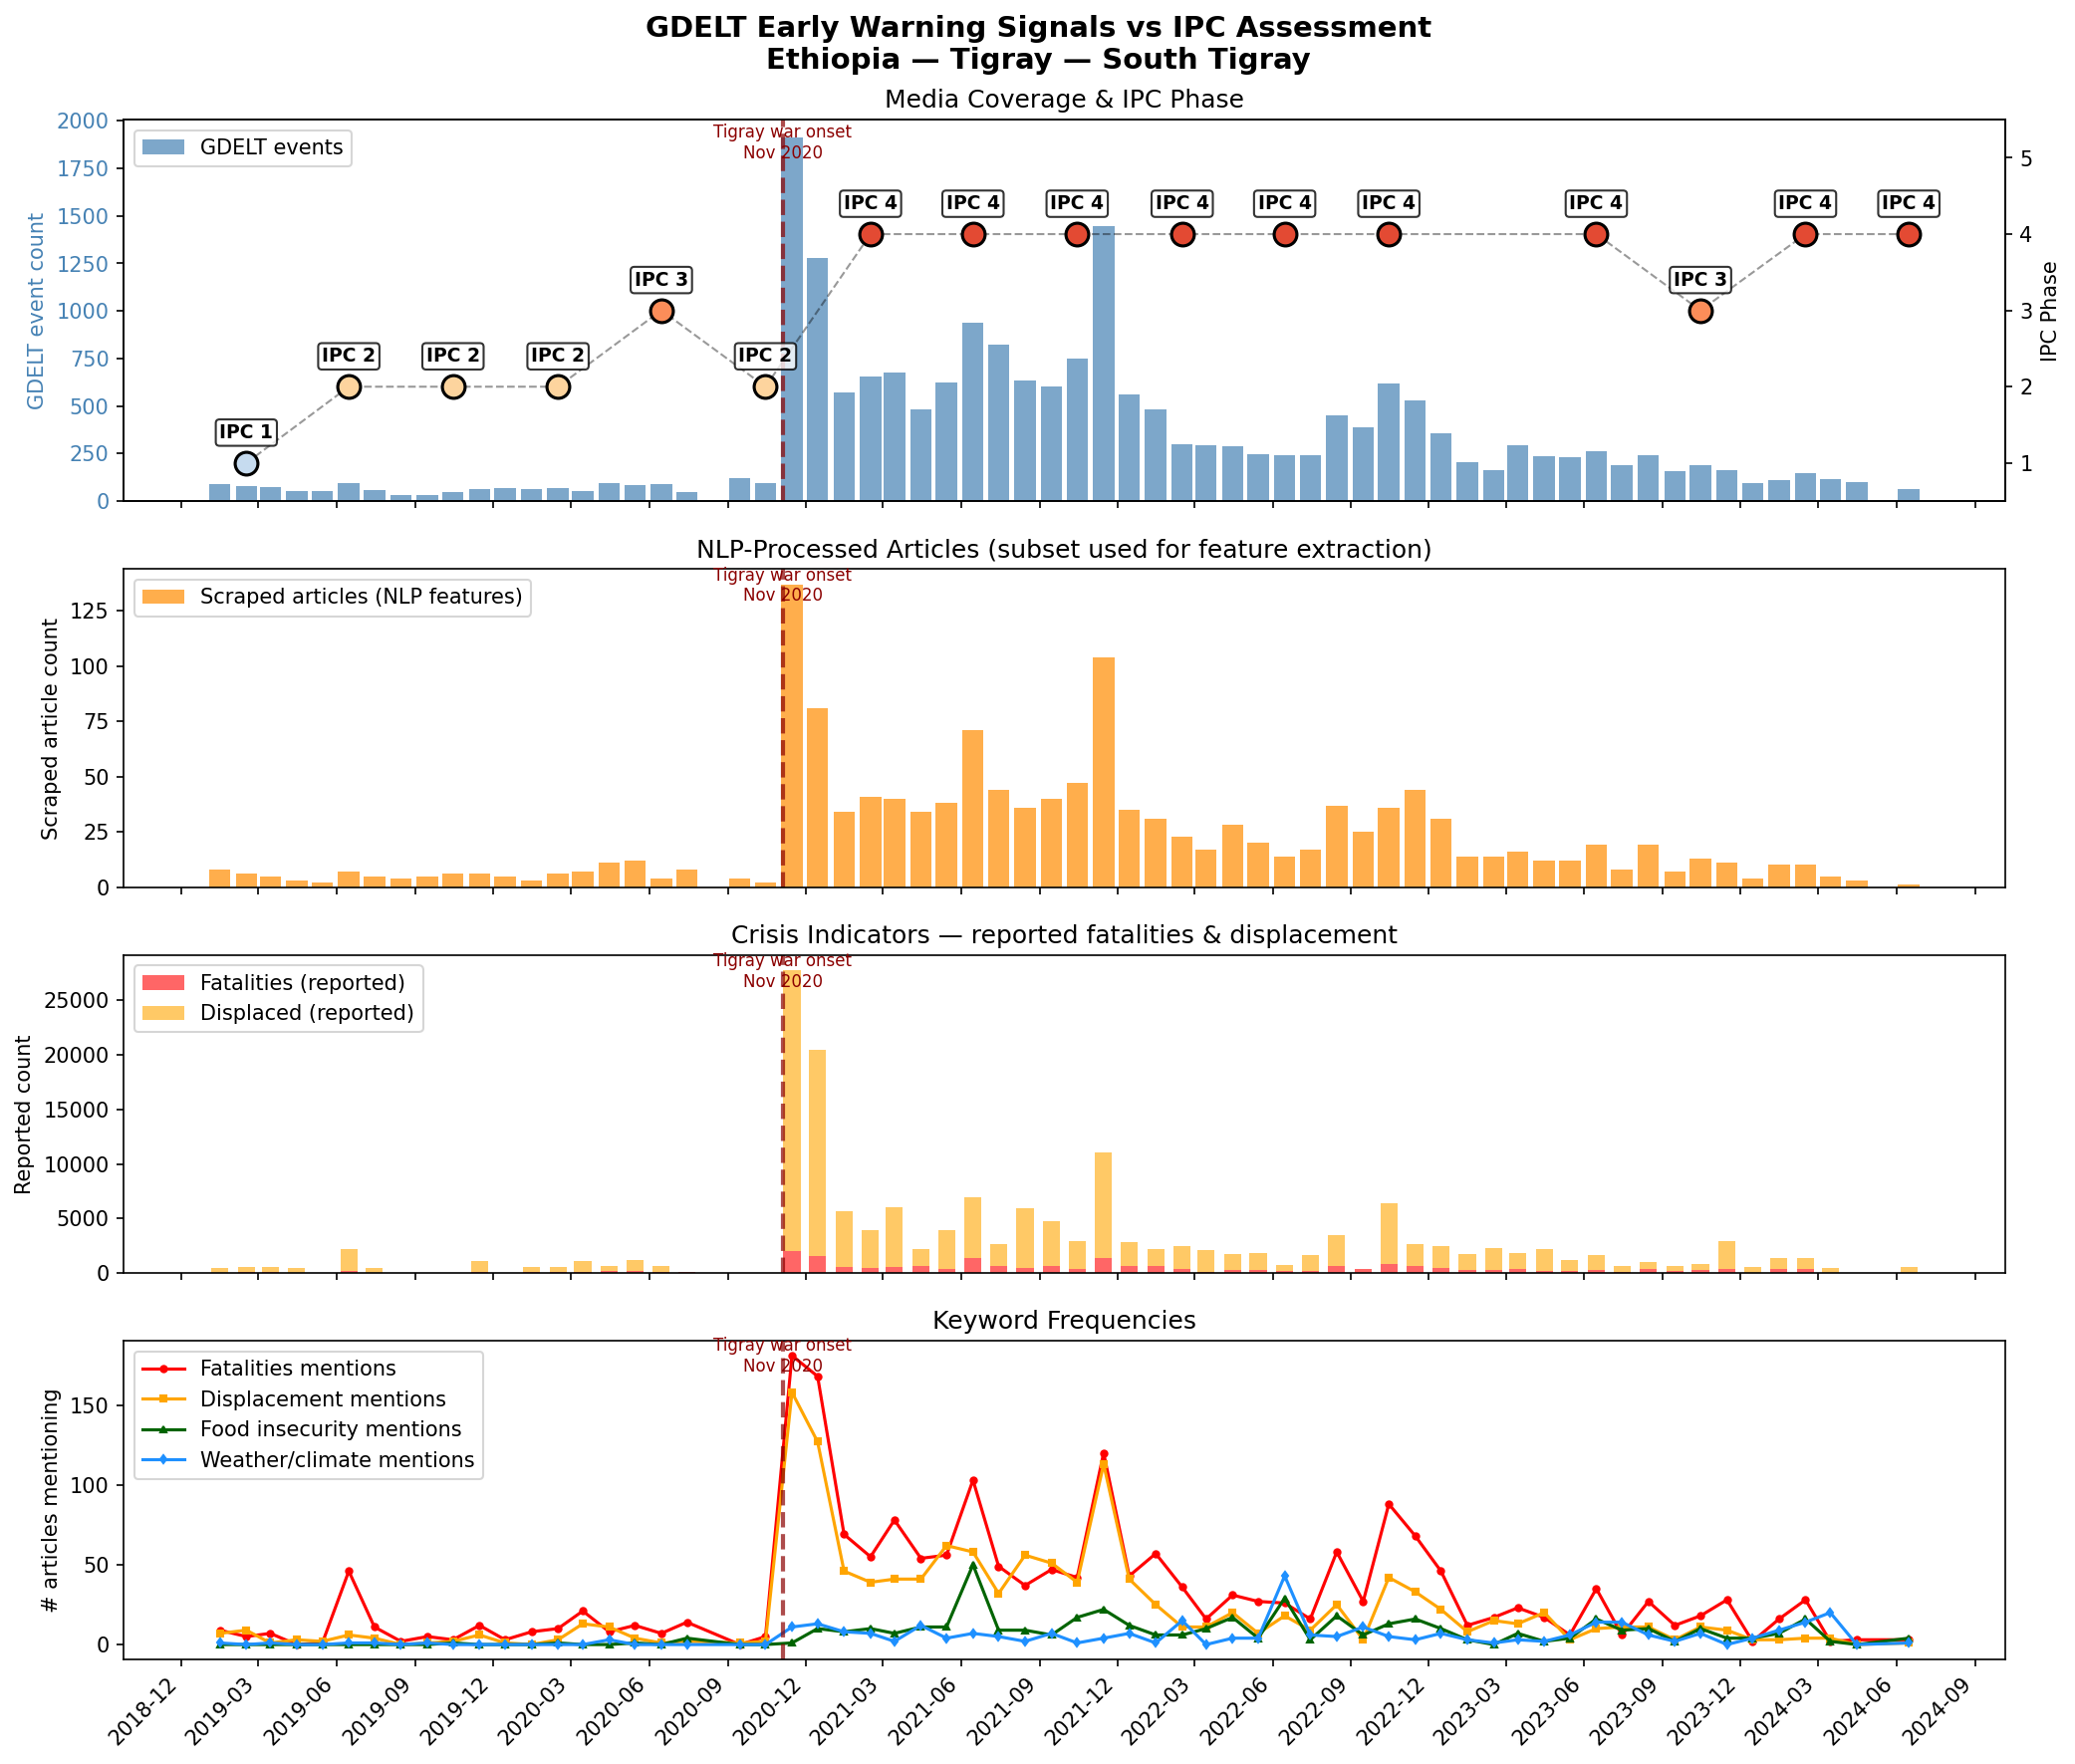
\includegraphics[width=\textwidth]{crisis_timeline_ethiopia_tigray_south_tigray.png}
    \caption{GDELT near-real-time media signals vs.\ IPC assessment timeline for South Tigray, Ethiopia. The vertical dashed line marks the onset of the Tigray conflict (November 2020).}
    \label{fig:case_ethiopia}
\end{figure}

\paragraph{Mozambique --- Dondo, Sofala (Cyclone Idai).}
Cyclone Idai made landfall near Beira on 14 March 2019 (Figure~\ref{fig:case_mozambique}), devastating Sofala province. Prior to the cyclone, Dondo was consistently at IPC~1 with minimal GDELT coverage ($<$50 events/month). The cyclone triggered an immediate spike: event counts exceeded 800, scraped articles jumped from near zero to over 60, and displacement counts surged above 5{,}000. Notably, \textit{weather/climate keyword mentions} peaked sharply alongside fatality and displacement signals, distinguishing this case from the conflict-driven crises. The IPC classification rose from 1 to 3 in the June 2019 assessment. This case demonstrates that GDELT captures climate-driven food security shocks with the same fidelity as conflict-driven ones, and that the weather-related features extracted from article text carry informative signal for natural-disaster scenarios.

\begin{figure}[H]
    \centering
    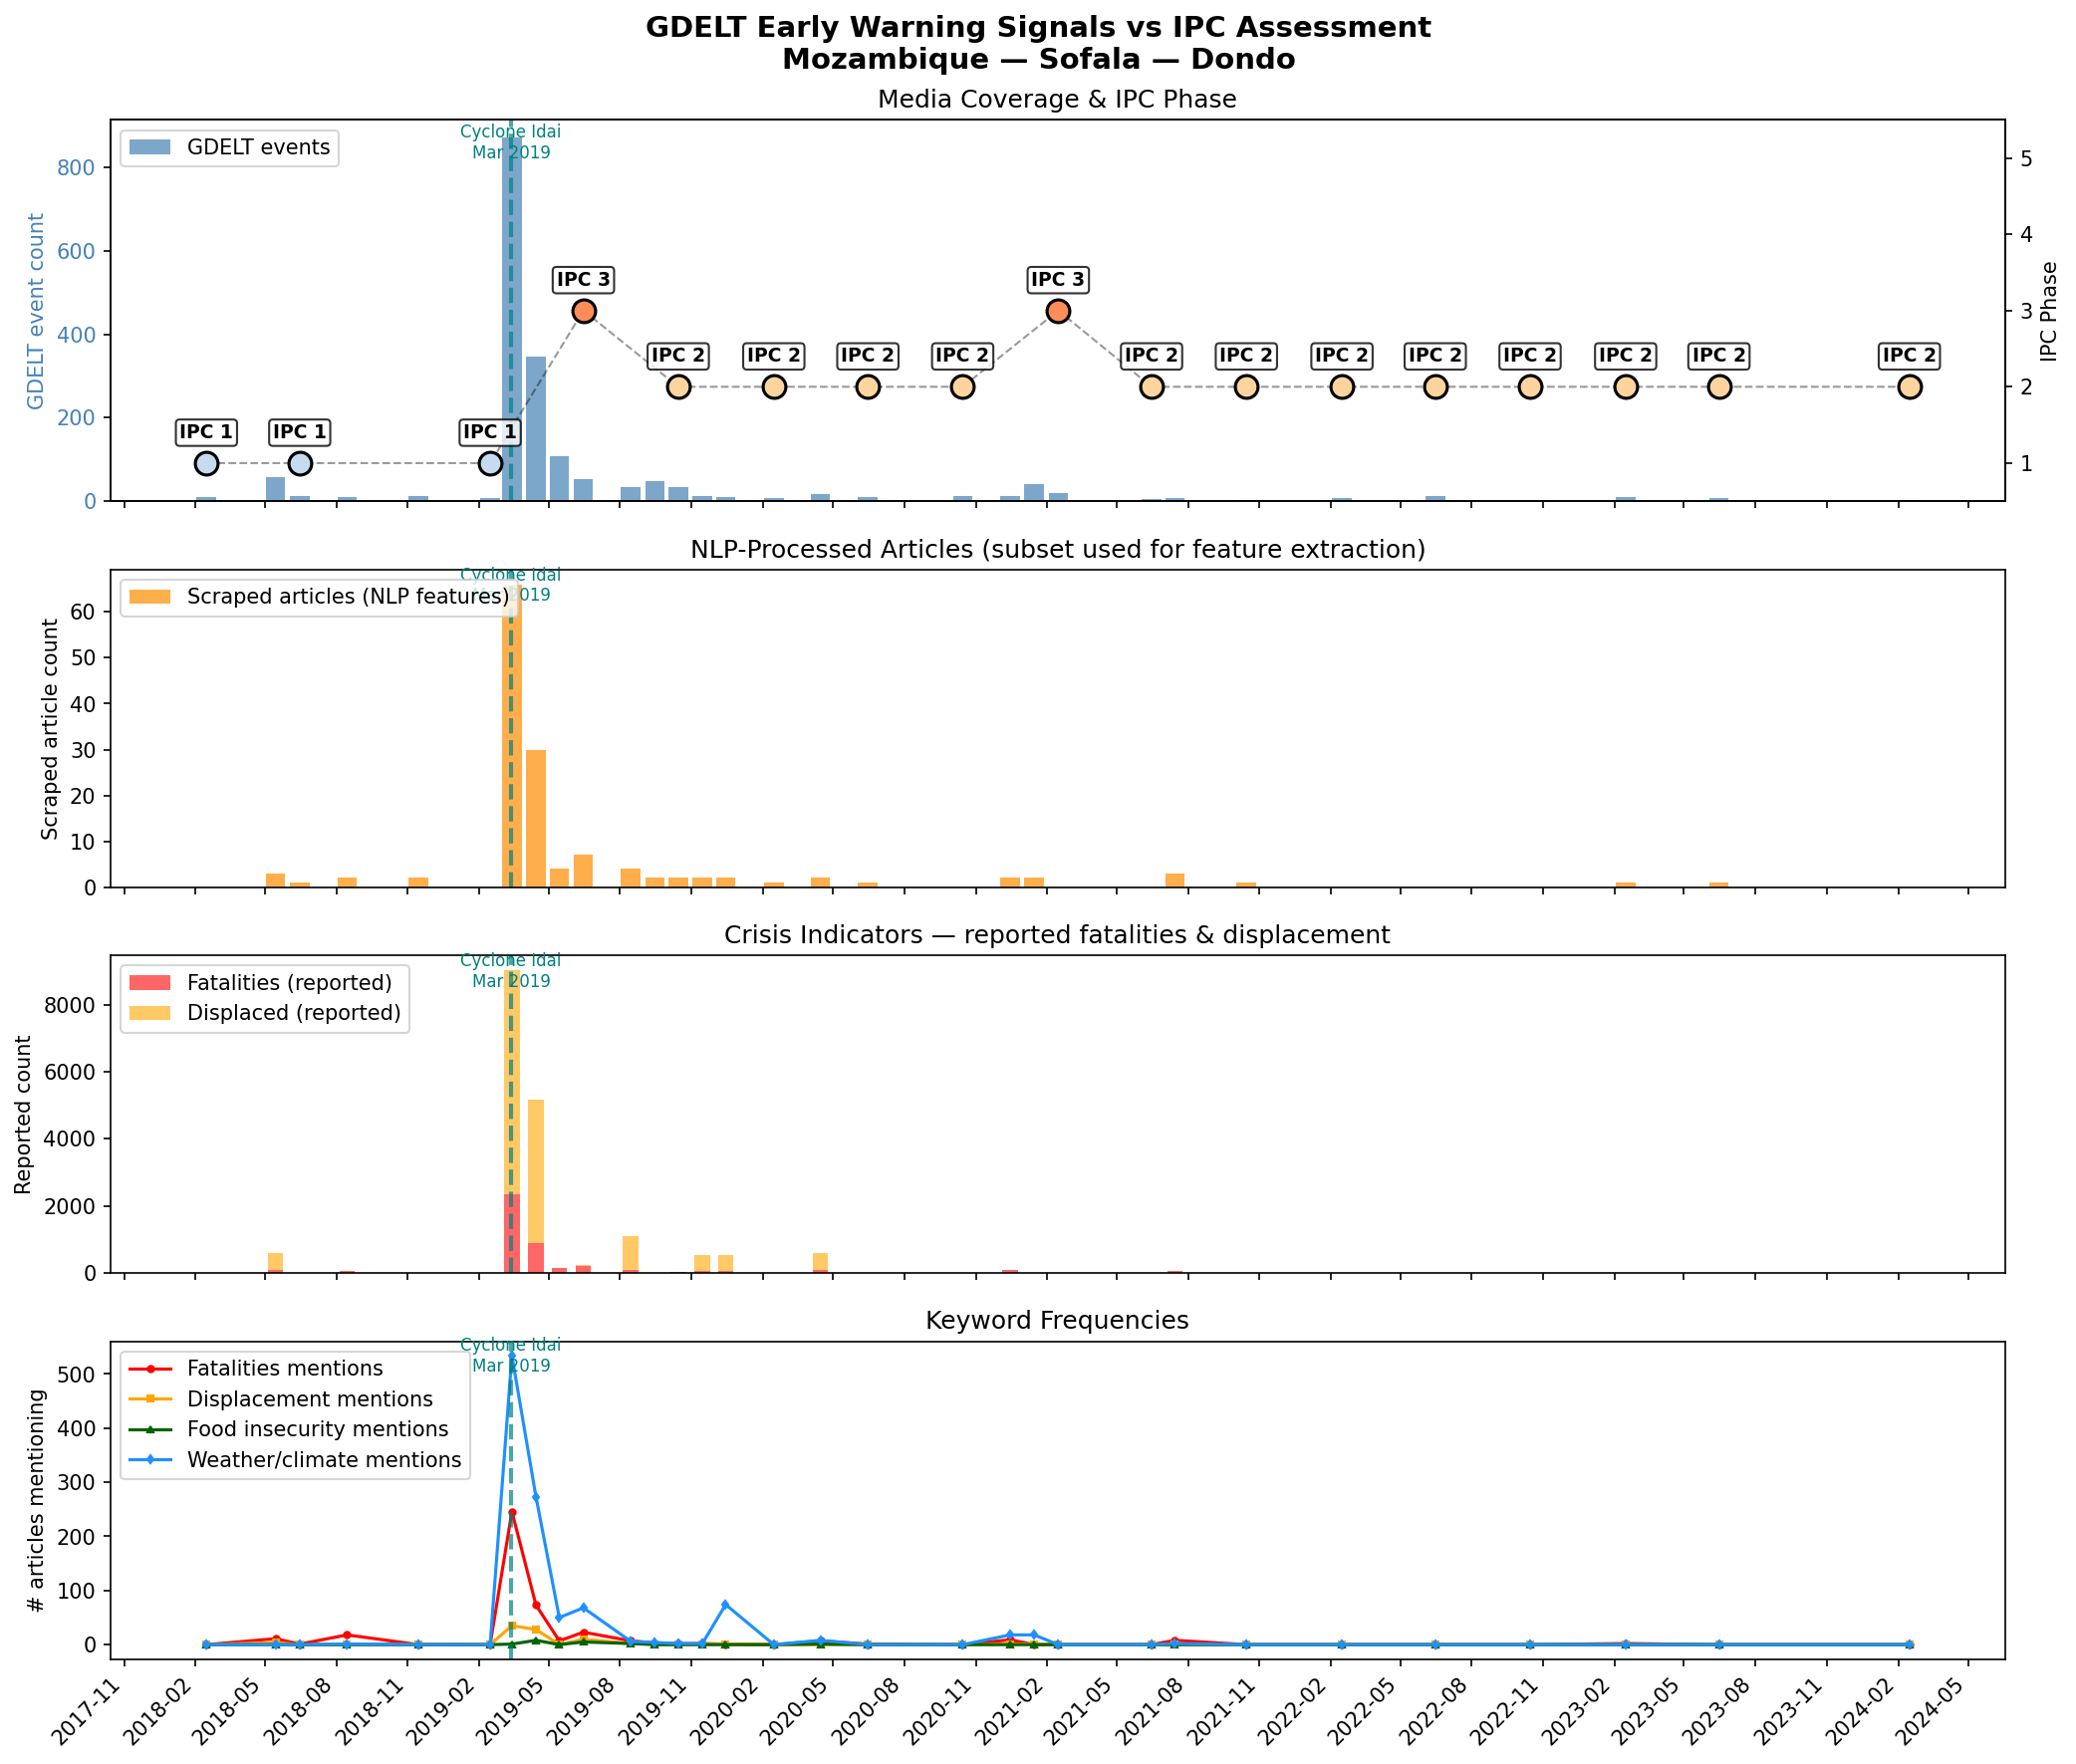
\includegraphics[width=\textwidth]{crisis_timeline_mozambique_sofala_dondo.png}
    \caption{GDELT near-real-time media signals vs.\ IPC assessment timeline for Dondo (Sofala), Mozambique. The vertical dashed line marks the landfall of Cyclone Idai (March 2019). Note the prominent weather/climate keyword signal in the bottom panel.}
    \label{fig:case_mozambique}
\end{figure}

\paragraph{Cross-case synthesis.}
The three cases map onto the temporal modes anticipated above: Sudan and Mozambique exhibit GDELT \emph{leading} IPC (by $\sim$12 months in Sudan, due to an assessment blackout, and by $\sim$3 months in Mozambique, as the cyclone spike preceded the June 2019 IPC update by an entire reporting cycle), while Ethiopia (Tigray) exhibits \emph{coincidence}, with the event-volume surge and the phase-2-to-4 IPC jump both occurring in the February 2021 window. None of the three cases shows news \emph{following} IPC; such cases plausibly exist (see Limitations) but are not represented in this selection. This pattern is consistent with the predictive modelling results showing that GDELT features can substitute for lagged IPC scores (Task~1) and provide increasing value at longer forecast horizons (Task~2). The cases also reveal differentiated signal signatures: conflict crises produce fatality- and displacement-dominated signals, while weather events generate distinct climate keyword patterns, suggesting that the feature space captures mechanistic information about crisis drivers, not merely generic ``bad news'' coverage.


\section{Discussion}

This study set out to assess whether open-source news data, processed through NLP pipelines, can provide operationally useful signals for food security analysis. The results offer a nuanced answer: GDELT-derived features are informative for \textit{level estimation} and \textit{nowcasting} of IPC phases, but contribute less to detecting \textit{directional changes} in food security status. In this section, we interpret these findings in the context of prior work, examine the mechanisms that may explain them, and discuss the practical implications and limitations of deploying news-based signals in humanitarian monitoring and nowcasting.

\subsection{Interpretation of Key Findings}

\paragraph{Substitutability of news signals for lagged IPC scores.}
The central finding of this study is that GDELT features combined with geographic context match the predictive performance of lagged IPC scores for level prediction (Task~1: F1 0.834 vs.\ 0.836 over all periods; 0.794 vs.\ 0.775 in recent periods). This result is consistent with Fraiberger et al.~\citep{Fraiberger2023}, who demonstrated that news-derived signals improve IPC forecasts, but goes further by showing that news features can \textit{substitute} for, rather than merely supplement, lagged IPC scores. The practical implication is significant: in settings where IPC assessments are delayed, disrupted, or entirely absent---as illustrated by the 12-month gap in Khartoum's assessment timeline---GDELT-derived features offer a viable near-real-time proxy for food security status.

The substitutability finding strengthens slightly over recent periods (2022--2024), where GDELT-only outperforms IPC-only by +0.020 F1 points. This temporal improvement aligns with documented expansions in GDELT's geographic coverage, linguistic processing capabilities, and source diversity over the past decade \citep{leetaru2013gdelt}. It suggests that the informational value of news-derived signals is not static but improves as underlying data quality increases---an encouraging trajectory for operational deployment. We caveat this trajectory, however: the 2022--2024 window coincides with several large geopolitical shocks (Sudan civil war, Ukraine-related supply disruptions, post-COVID inflation) that simultaneously elevate media volume and food security severity in our sample, so the recent-period gain may partly reflect these episodes' high news salience rather than a generalisable improvement in the GDELT signal itself.

\paragraph{Increasing value at longer forecast horizons.}
At the two-assessment-ahead horizon ($\sim$8 months), GDELT-only features outperform IPC-only even over the full evaluation window (F1 0.746 vs.\ 0.740). This result has a straightforward interpretation: as the most recent IPC score becomes stale, its predictive power for future conditions diminishes, while continuously updated news signals retain their ability to reflect current dynamics. This finding supports the theoretical motivation advanced by Ahn et al.~\citep{Ahn2023} and others for integrating streaming media data into monitoring systems, and extends it by providing direct empirical evidence of the crossover point at which news features become more informative than expert classifications.

\paragraph{Why transition prediction resists improvement.}
The failure of GDELT features to improve transition prediction (Task~3) deserves careful interpretation. We argue this reflects a structural property of news-derived data rather than a methodological limitation. Food security transitions---particularly worsenings---are relatively rare events ($\sim$12--17\% of observations) driven by the interaction of slow-moving structural vulnerabilities (poverty, governance, infrastructure) with acute shocks (conflict, drought, price spikes). News media primarily captures the latter: acute, visible events that generate coverage. However, whether such shocks translate into IPC deterioration depends critically on pre-existing vulnerability, which news signals do not encode. The strong performance of IPC-only for transitions (F1 0.718) confirms that the best predictor of whether conditions will worsen is \textit{where they currently stand}---a piece of information already embedded in the most recent IPC score and geographic fixed effects.

This interpretation is reinforced by the collapse of GDELT-only performance for transitions (F1 0.445), compared to its strong showing for level prediction (F1 0.834). News-derived features capture \textit{what is happening} (severity of crisis) but not \textit{what will change} (direction of movement), a distinction that has direct implications for how media-derived signals should be deployed in operational systems.

\paragraph{The essential role of geographic context.}
Across all tasks, removing geographic dummy variables caused GDELT-based model performance to collapse (F1 $\sim$0.33--0.39). This finding underscores that news signals are inherently relative rather than absolute: the same volume of conflict reporting may correspond to IPC~2 in one country and IPC~4 in another, depending on baseline vulnerability, media market structure, and reporting norms. Geographic fixed effects effectively calibrate the news signal to local context. This result has practical implications for system design: any operational deployment of news-based food security monitoring must incorporate spatial context, either through explicit location encoding or through models that learn region-specific baselines.

\subsection{Relation to Prior Work}

Our findings extend and qualify several strands of prior research. Fraiberger et al.~\citep{Fraiberger2023} demonstrated that news-derived features reduce IPC forecast error by over 40\%, but their evaluation combined news features with other inputs (weather, prices) rather than testing substitutability directly. Our controlled feature-set comparison isolates the contribution of news signals and shows they can stand alone with geographic context. Ahn et al.~\citep{Ahn2023} showed that transformer-based models trained on news text outperform expert indicator baselines, but their \textit{HungerGist} system operated at the country level. Our ADMIN2-level analysis demonstrates that news signals retain predictive value at finer spatial scales, though with the caveat that geographic encoding is essential.

The diagnostic comparison of GDELT Events and GKG data also contributes to the emerging literature on media data quality for humanitarian applications. Consistent with Valentin et al.~\citep{Valentin2024}, who emphasised the importance of correcting for uneven media coverage, we find that the Events stream provides broader and more temporally responsive coverage than the GKG, while the GKG captures richer narrative content where coverage exists. The regression analysis showing a significant positive association between Events article volume and IPC severity (but not for GKG) suggests that event-coded data more reliably tracks the intensity dimension of food security crises.

\subsection{Limitations}

Several limitations qualify the interpretation and generalisability of our findings.

\paragraph{Media coverage bias.}
GDELT coverage is neither random nor uniform. Countries and regions that receive sustained international media attention (e.g., Sudan, Somalia, Ethiopia) are over-represented, while equally severe crises in less visible areas may go underreported. Our geographic fixed effects partially mitigate this by learning region-specific baselines, but cannot fully correct for systematic under-coverage in data-scarce areas. The case studies illustrate this: the three selected areas all had substantial GDELT coverage, and the approach's utility in regions with minimal media presence remains unvalidated.

\paragraph{Endogeneity concerns.}
Media attention may respond to, rather than anticipate, food security deterioration. While the case study timelines suggest that GDELT signals spike at or shortly after crisis onset---often before IPC assessments are published---we cannot rule out the possibility that some signals are contemporaneous with, rather than leading, the underlying conditions. The predictive modelling framework mitigates this through strict temporal separation (rolling windows with no look-ahead), but the distinction between leading and coincident signals has implications for the practical ``early warning'' framing.

\paragraph{Label quality.}
IPC classifications are expert assessments, not direct measurements. They incorporate judgement, scenario modelling, and information constraints, which may introduce noise or systematic bias into the ground-truth labels. Furthermore, the irregularity of IPC assessment cycles (approximately 3 times per year) means that the true trajectory of food security conditions between assessments is unobserved, limiting the temporal resolution at which any model can be evaluated. A second, distinct label-quality concern affects the intermediate text features rather than the IPC targets: the MultiTaskBERT impact, urgency, and resource signals are trained on LLM-generated (weak-supervision) labels validated only on a small, non-independent 5\% sample. These features may therefore inherit biases from the labelling model, and should be regarded as noisy auxiliary signals rather than verified annotations; establishing their validity against a human-labelled gold standard is left to future work.

\paragraph{Model simplicity.}
The linear dominance of Logistic Regression across all tasks suggests that the current feature space may not benefit from more complex nonlinear modelling. While this simplicity is a practical advantage (LR models are fast, interpretable, and robust to overfitting), it also suggests that the feature engineering may not yet capture interactions or higher-order patterns that tree-based models could exploit. Future work with larger and more diverse datasets may benefit from deeper architectures.

\paragraph{Temporal scope.}
The evaluation window (2016--2024) is constrained by the availability of consistent FEWS NET and GDELT data. The finding that GDELT performance improves in recent periods is encouraging but also means that the strongest results are based on a relatively small number of evaluation folds (6 periods for the recent-period analysis), limiting statistical power.

\subsection{Implications for Operational Monitoring}

Despite these limitations, the findings have concrete implications for how news-derived signals could be integrated into food security monitoring:

\begin{enumerate}
    \item \textbf{Gap-filling between IPC cycles.} The substitutability result suggests that GDELT-based models could provide interim food security estimates during the months between IPC assessment cycles, offering continuous monitoring where only periodic snapshots currently exist. The Sudan case study demonstrates the value of this capability during assessment disruptions.

    \item \textbf{Rapid deployment in new crises.} When a new crisis emerges in an area without recent IPC scores, GDELT signals combined with geographic context could provide an immediate estimate of food security severity. This is particularly relevant for sudden-onset disasters (as in the Mozambique case) where formal assessment processes take weeks to months to produce official classifications.

    \item \textbf{Signal differentiation by crisis type.} The case studies show that GDELT features capture not only the \textit{intensity} of a crisis but also its \textit{type}---conflict-driven crises generate fatality- and displacement-dominated signals, while climate events produce distinct weather keyword patterns. This differentiation could inform response planning by signalling not just \textit{that} conditions are deteriorating but \textit{why}, enabling more targeted resource allocation.

    \item \textbf{Complementary rather than competing.} The results do not suggest that GDELT should replace IPC assessments---which remain the gold standard for food security classification---but rather that news-derived signals occupy a complementary niche: they are available in near-real-time, at low cost, and at scale, while IPC assessments provide authoritative but infrequent and resource-intensive expert judgement. A hybrid system that combines both would inherit the strengths of each.
\end{enumerate}


\section{Conclusion}

This study investigated the potential of open-source news data, processed through NLP pipelines, to serve as an input for food security analysis and prediction. Using GDELT's Event and Global Knowledge Graph datasets aligned with FEWS NET IPC classifications across African countries, we conducted a systematic evaluation spanning diagnostic media analysis, multi-task predictive modelling, and qualitative case studies.

Three principal contributions emerge. First, we demonstrate that GDELT-derived features combined with geographic context can \textit{substitute} for lagged IPC scores in predicting food security levels, achieving equivalent performance over all periods (F1 0.834 vs.\ 0.836) with a small recent-period edge (0.794 vs.\ 0.775 in 2022--2024). This substitution should be read with two important caveats: it holds only when geographic identifiers are included, as GDELT features in isolation are substantially weaker predictors, so geography---not news content alone---carries much of the signal; and the recent-period advantage rests on a short (2022--2024) evaluation window that coincides with major geopolitical shocks (Sudan civil war, Ukraine-related supply disruptions, post-COVID inflation), and we therefore interpret it cautiously rather than as established forecast skill. This finding has direct operational relevance for regions with delayed, disrupted, or absent official assessments. Second, we show that the informational advantage of news signals increases at longer forecast horizons, where lagged IPC scores become stale---supporting the integration of streaming media data into medium-term early warning applications. Third, through case studies spanning three countries and three crisis drivers (civil war, regional conflict, and cyclone), we provide qualitative evidence that GDELT signals spike at or immediately following crisis onset, often before IPC assessments are updated, and that the feature space captures differentiated crisis signatures.

The study also delineates clear boundaries. News-derived features encode information about food security \textit{levels} rather than \textit{transitions}, and geographic context is essential for calibrating media signals to local conditions. These findings imply that GDELT-based models are best suited for nowcasting and level estimation---complementing rather than replacing expert-led assessment systems---and that future work should focus on integrating news signals with other near-real-time data streams (e.g., satellite imagery, market prices) to address the limitations of any single source.

More broadly, this work contributes to the growing body of evidence that unstructured text, processed at scale through NLP, can provide timely and interpretable signals for humanitarian monitoring. As GDELT's coverage continues to expand and NLP capabilities improve, the substitutability demonstrated here is likely to strengthen, offering a scalable pathway toward more responsive near-real-time food security early warning in data-scarce settings.

\newpage
\bibliographystyle{elsarticle-num}
\bibliography{sources}

\appendix

\section{Supplementary Figures: IPC Phase Heatmaps}

\begin{figure}[H]
    \centering
    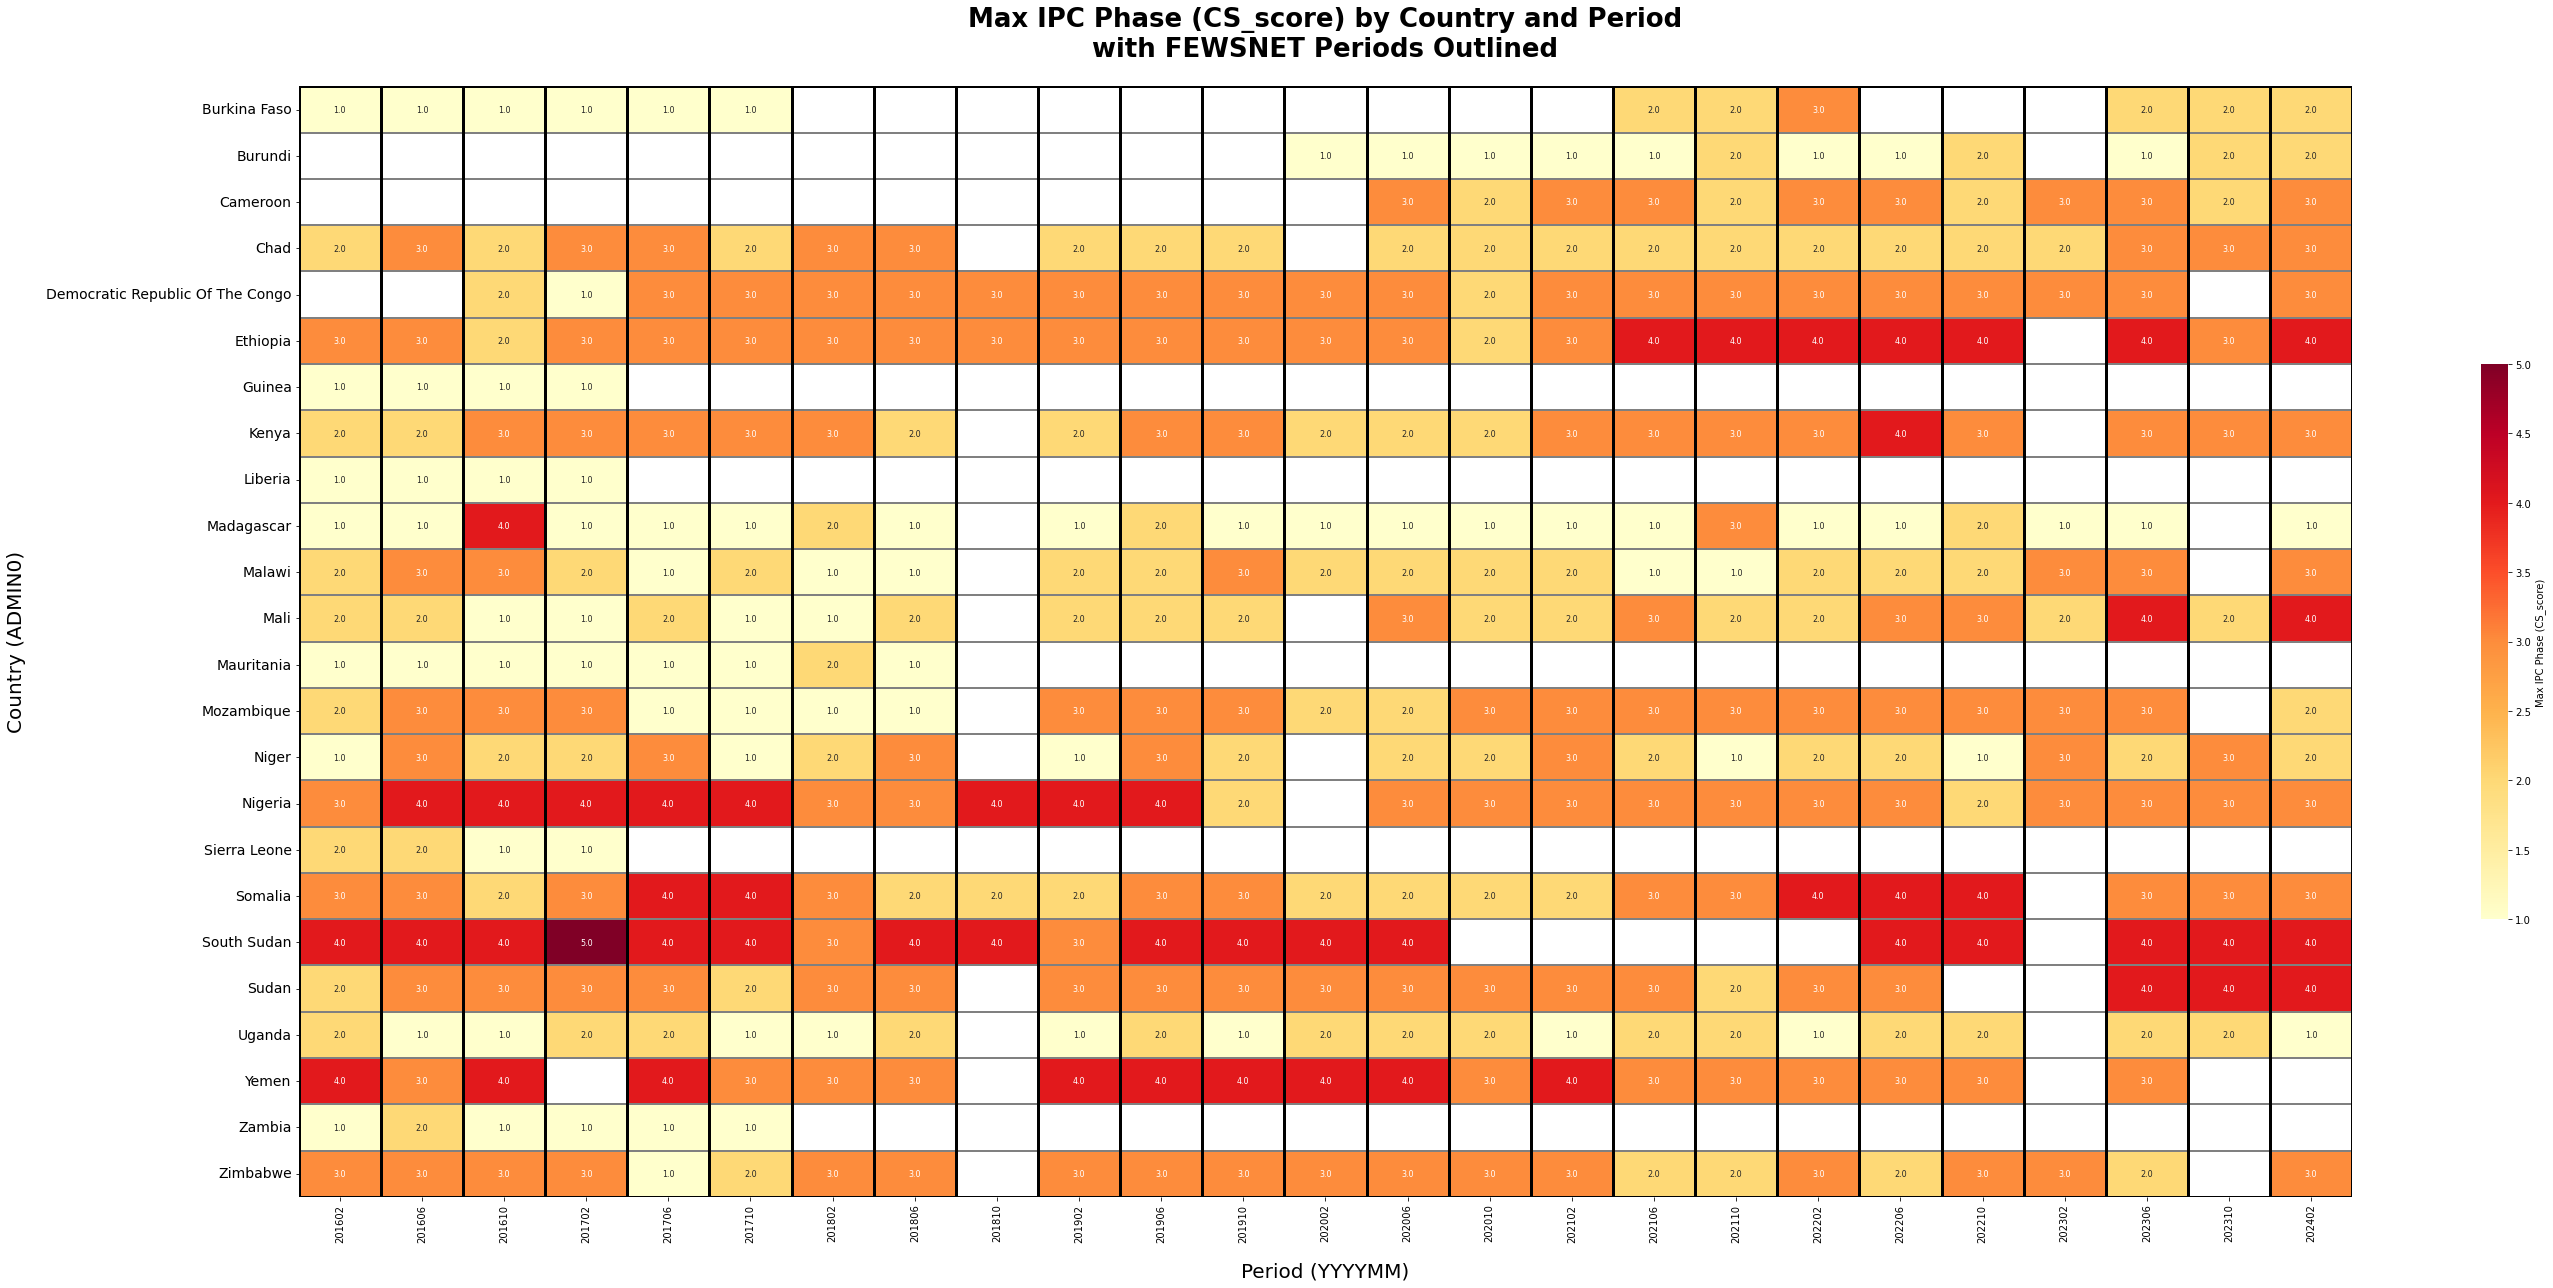
\includegraphics[width=\textwidth]{max_ipc.png}
    \caption{\textbf{S1: Maximum IPC phase by country and FEWS NET period.} Each cell reports the highest IPC phase (1--5) observed in any subnational unit within a country for each reporting round. Bold outlines indicate official FEWS NET analysis periods.}
\end{figure}

\begin{figure}[H]
    \centering
    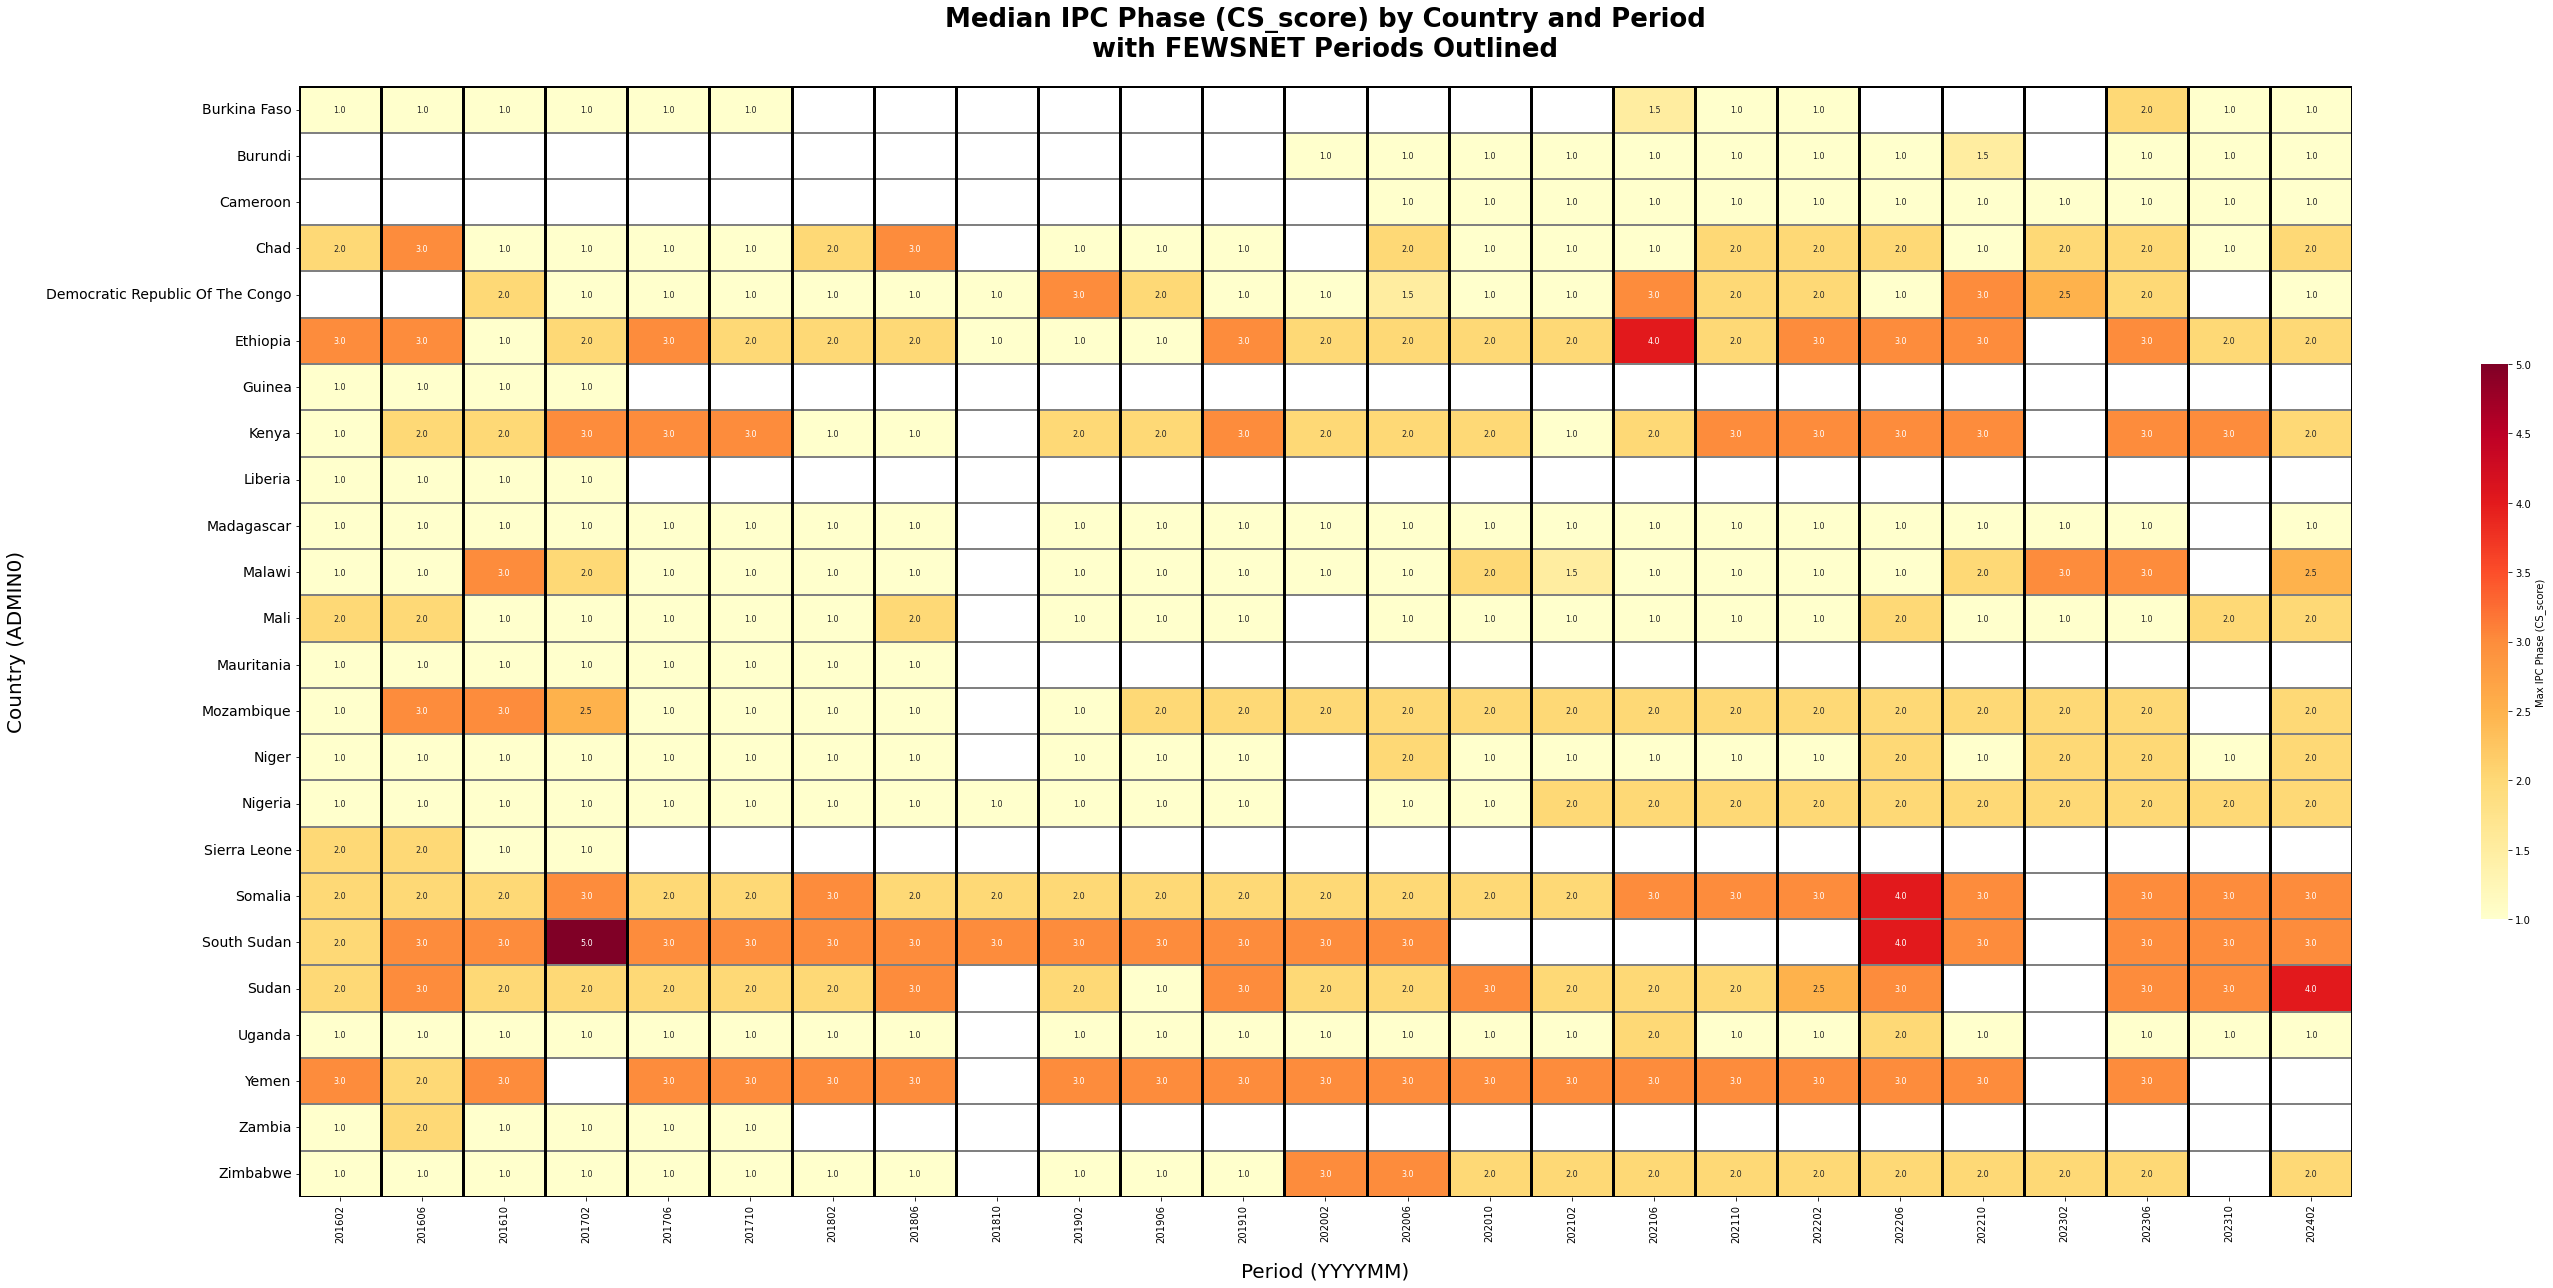
\includegraphics[width=\textwidth]{median_ipc.png}
    \caption{\textbf{S2: Median IPC phase by country and FEWS NET period.} Each cell shows the median IPC phase across all reporting subnational units per country and round, providing a robust central tendency for national food insecurity status.}
\end{figure}

\section{Supplementary Figures: Article Count Diagnostics}

\begin{figure}[H]
\centering
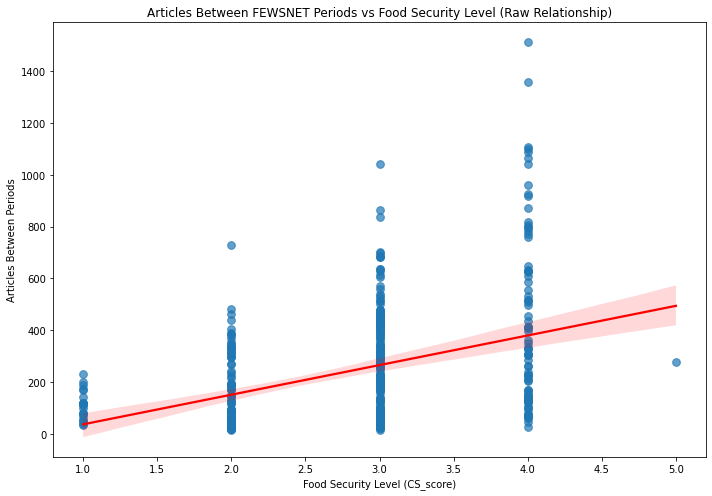
\includegraphics[width=0.48\textwidth]{events_raw_scatter.png}
\hfill
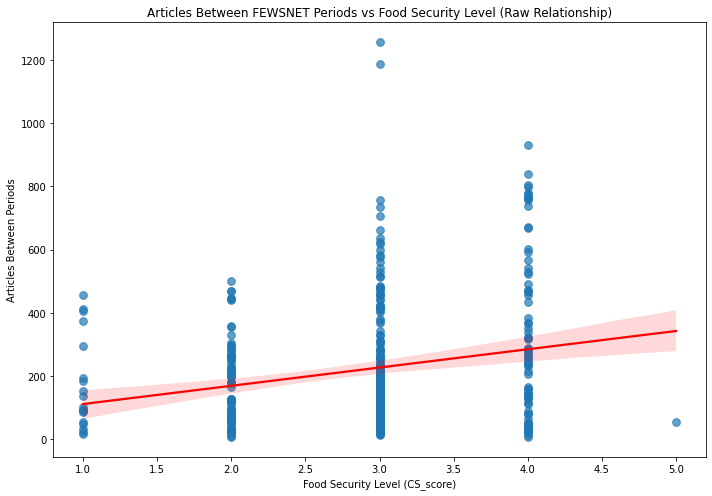
\includegraphics[width=0.48\textwidth]{gkg_raw_scatter.png}
\caption{\textbf{S3: Relationship between article counts and IPC phase (CS score).} \textbf{Left:} GDELT Events. \textbf{Right:} GDELT GKG. Each point is a country-period; lines indicate OLS linear fits without fixed effects.}
\label{fig:appendix_raw_scatter}
\end{figure}

\begin{figure}[H]
\centering
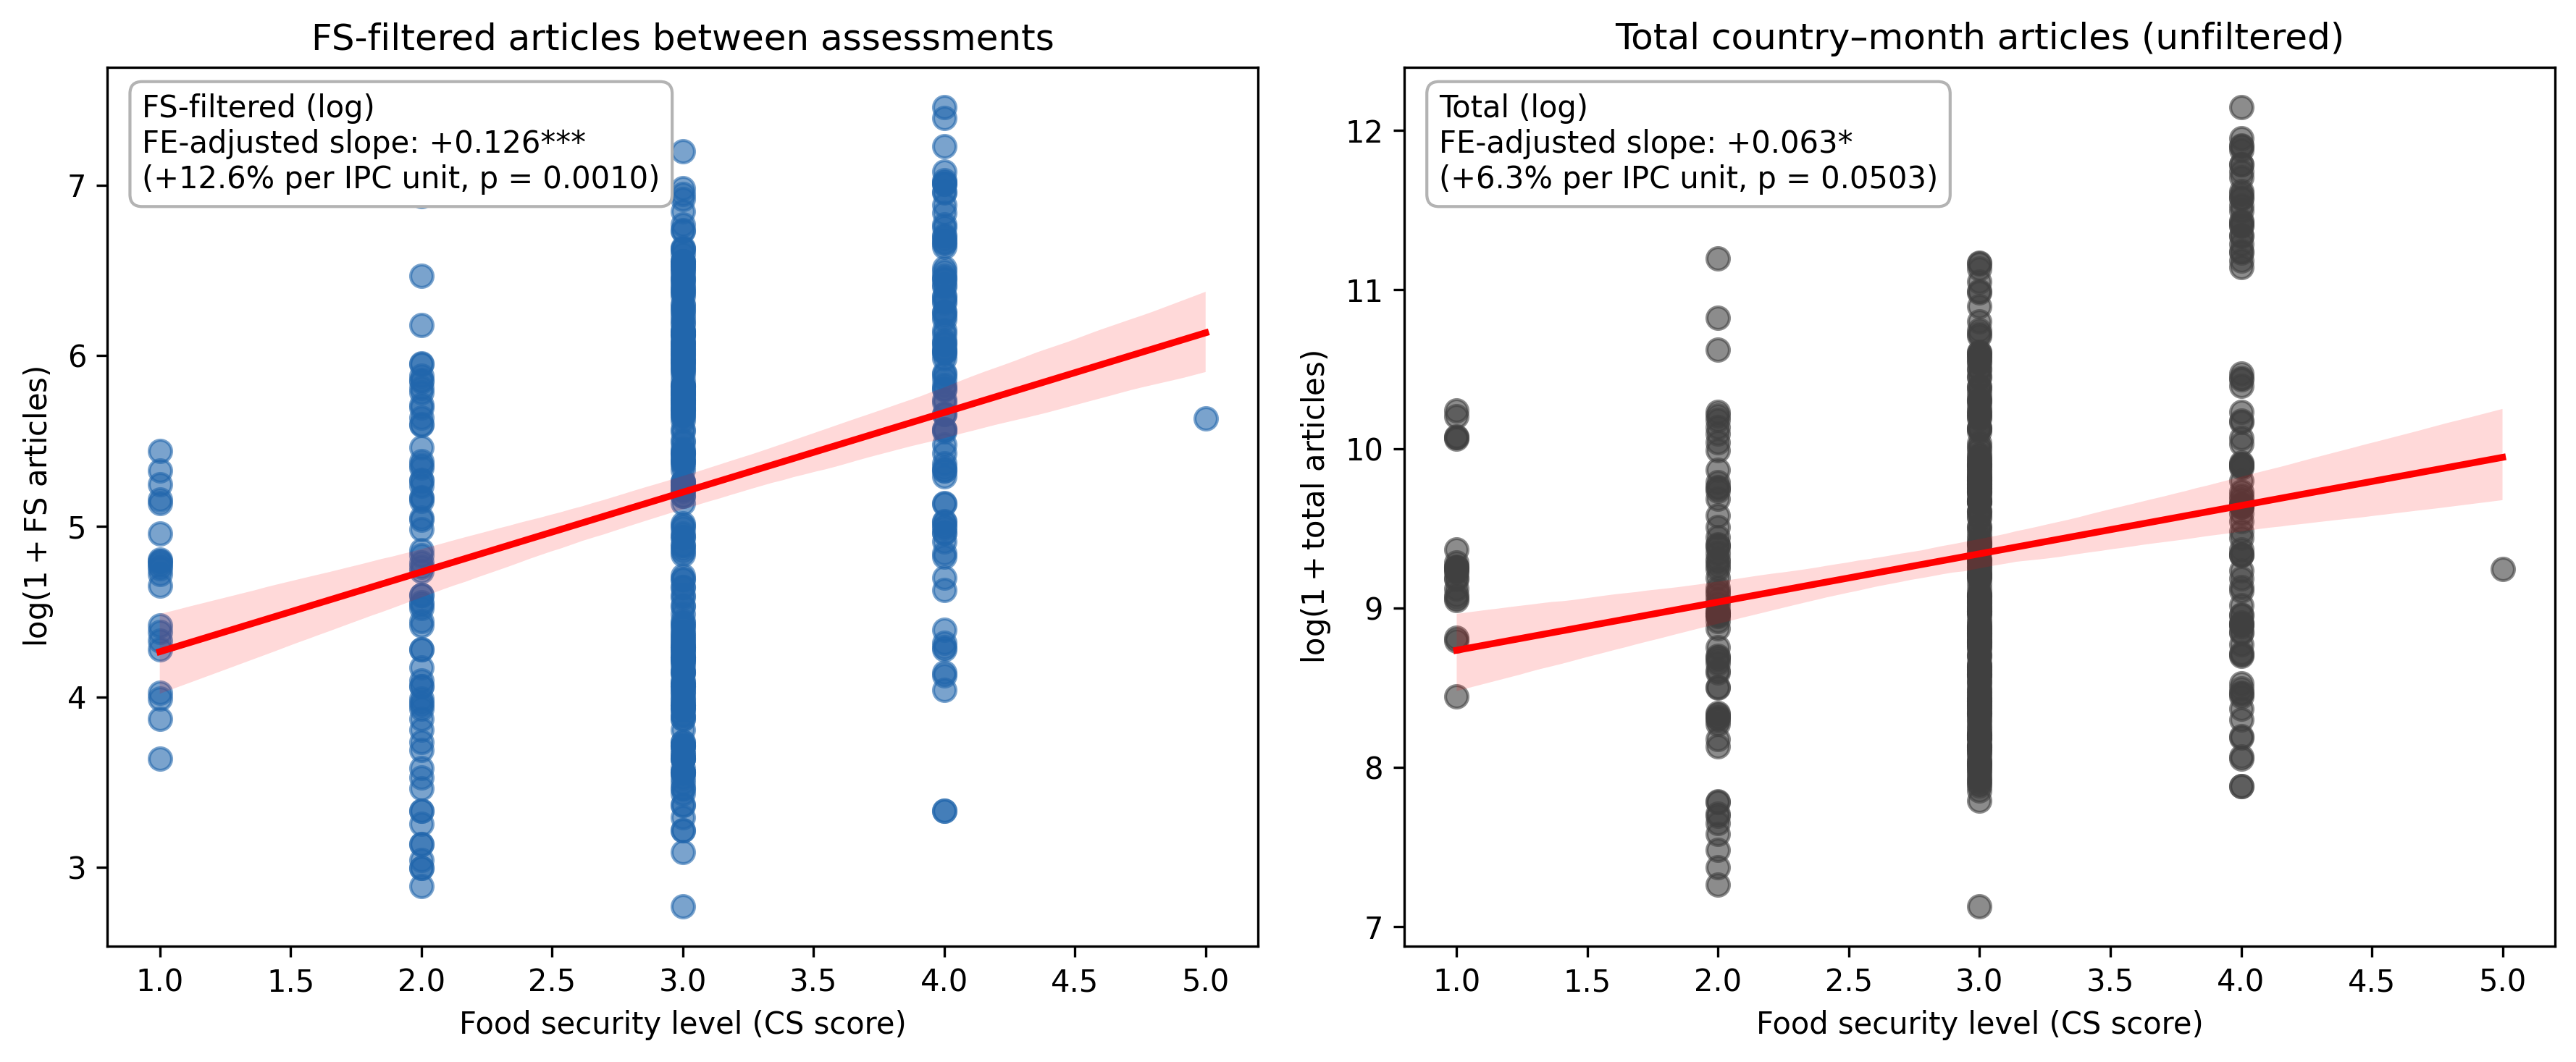
\includegraphics[width=\textwidth]{log_articles_vs_cs.png}
\caption{\textbf{S4: Proportional response of news volume to IPC severity (GDELT Events).} Each point is a country–period observation; the red line is a raw OLS fit (without fixed effects). The boxed annotation reports the country- and period-FE-adjusted semi-elasticity from the panel regression $\log(1+\text{articles}) \sim \text{CS\_score} + C(\text{ADMIN0}) + C(\text{period})$, restricted to country-months with non-zero total volume ($N=404$). \textbf{Left:} food-security-keyword-filtered articles (CAMEO-screened). \textbf{Right:} total country–month articles (unfiltered, pulled from the public \texttt{gdelt-bq.gdeltv2.events} dataset). At the country-month aggregation, FS-filtered news rises by approximately $+12.6\%$ per IPC phase ($p<0.01$), roughly twice the proportional response of total country-month news ($+6.3\%$ per IPC phase, $p\approx0.05$). The keyword filter therefore amplifies the proportional response of news activity to food security severity, particularly in low-baseline-coverage countries that level regressions implicitly downweight.}
\label{fig:appendix_log_scatter}
\end{figure}

\section{Supplementary Tables: Regression Diagnostics}
\begin{table}[H]
\centering
\caption{Association between article counts and IPC CS scores. Each column shows results from OLS regressions with country and period fixed effects. Standard errors in parentheses. $^{***}p<0.01$.}
\begin{tabular}{lcc}
\toprule
 & Events & GKG \\
\midrule
CS score & 33.5*** & --20.5 \\
 & (12.6) & (11.0) \\
Country FE & Yes & Yes \\
Period FE & Yes & Yes \\
Observations & 404 & 379 \\
$R^2$ & 0.76 & 0.77 \\
\bottomrule
\end{tabular}
\label{tab:appendix_regression_summary}
\end{table}

\begin{table}[H]
\centering
\caption{Lead-lag diagnostic: today's FS-filtered article volume predicting the IPC CS score at the $k$th next observed assessment ($k=1,\dots,4$). Two specifications per horizon: (a) GDELT only; (b) controlling for today's IPC (\texttt{CS\_score}). All columns include country and period fixed effects on the same panel as Table~\ref{tab:appendix_regression_summary}. Coefficients on \texttt{articles\_between} are reported in their natural units (per article) and rounded to three decimals; a 100-article shift therefore corresponds to coefficient $\times 100$ in IPC phase units. Coef (p-value); $^{***}p<0.01$, $^{**}p<0.05$, $^{*}p<0.10$.}

\begin{tabular}{lcccc}
\toprule
 & $k=1$ & $k=2$ & $k=3$ & $k=4$ \\
\midrule
\multicolumn{5}{l}{\emph{(a) cs\_next$_k$ $\sim$ articles\_between $+$ FE}} \\
articles\_between & $+0.001^{***}$ & $+0.000^{***}$ & $+0.000^{*}$ & $+0.000^{*}$ \\
                  & $(0.000)$ & $(0.006)$ & $(0.062)$ & $(0.065)$ \\
$R^2$             & $0.616$ & $0.597$ & $0.576$ & $0.571$ \\
\addlinespace
\multicolumn{5}{l}{\emph{(b) cs\_next$_k$ $\sim$ articles\_between $+$ CS\_score $+$ FE}} \\
articles\_between & $+0.000^{***}$ & $+0.000^{**}$ & $+0.000$ & $+0.000^{*}$ \\
                  & $(0.005)$ & $(0.021)$ & $(0.159)$ & $(0.085)$ \\
CS\_score         & $+0.350^{***}$ & $+0.183^{***}$ & $+0.165^{***}$ & $+0.030$ \\
                  & $(0.000)$ & $(0.001)$ & $(0.002)$ & $(0.586)$ \\
$R^2$             & $0.664$ & $0.610$ & $0.589$ & $0.571$ \\
$N$               & $393$ & $369$ & $345$ & $324$ \\
\bottomrule
\end{tabular}

\label{tab:lead_lag_diagnostic}
\end{table}

\section{Supplementary Tables: MultiTaskBERT Training Metrics}

\begin{sidewaystable}
\centering
\caption{MultiTaskBERT training and validation metrics per epoch. Training loss is averaged over all logging steps within each epoch. Validation loss and task-specific metrics are computed on the held-out stratified validation set at the end of each epoch.}
\label{tab:bert_training_metrics}
\begin{tabular}{rcccccc}
\toprule
Epoch & Training Loss & Validation Loss & Impact Acc & Urgency Acc & Resource F1 Micro & Resource F1 Macro \\
\midrule
1  & 1.3042 & 1.8254 & 0.7253 & 0.7986 & 0.8566 & 0.7353 \\
2  & 0.7016 & 1.9595 & 0.7471 & 0.7995 & 0.8616 & 0.7409 \\
3  & 0.4716 & 2.4037 & 0.7465 & 0.7997 & 0.8674 & 0.7678 \\
4  & 0.3142 & 2.8250 & 0.7511 & 0.7897 & 0.8746 & 0.7816 \\
5  & 0.2124 & 2.9301 & 0.7558 & 0.7898 & 0.8795 & 0.8090 \\
6  & 0.2394 & 3.0570 & 0.7481 & 0.7761 & 0.8922 & 0.8095 \\
7  & 0.1879 & 3.3721 & 0.7509 & 0.7793 & 0.8918 & 0.8274 \\
8  & 0.1375 & 3.4898 & 0.7460 & 0.7851 & 0.8928 & 0.8300 \\
9  & 0.1026 & 3.5946 & 0.7475 & 0.7849 & 0.8971 & 0.8430 \\
10 & 0.0803 & 3.5668 & 0.7471 & 0.7906 & 0.8944 & 0.8428 \\
\bottomrule
\end{tabular}
\end{sidewaystable}

\section{Supplementary Figures: GDELT Events Diagnostics}

This appendix presents diagnostic heatmaps for key features extracted from GDELT Events data (2017–2024) across ADMIN2 regions and monthly periods. See main text Section~2 for summary discussion.

\begin{figure}[H]
    \centering
    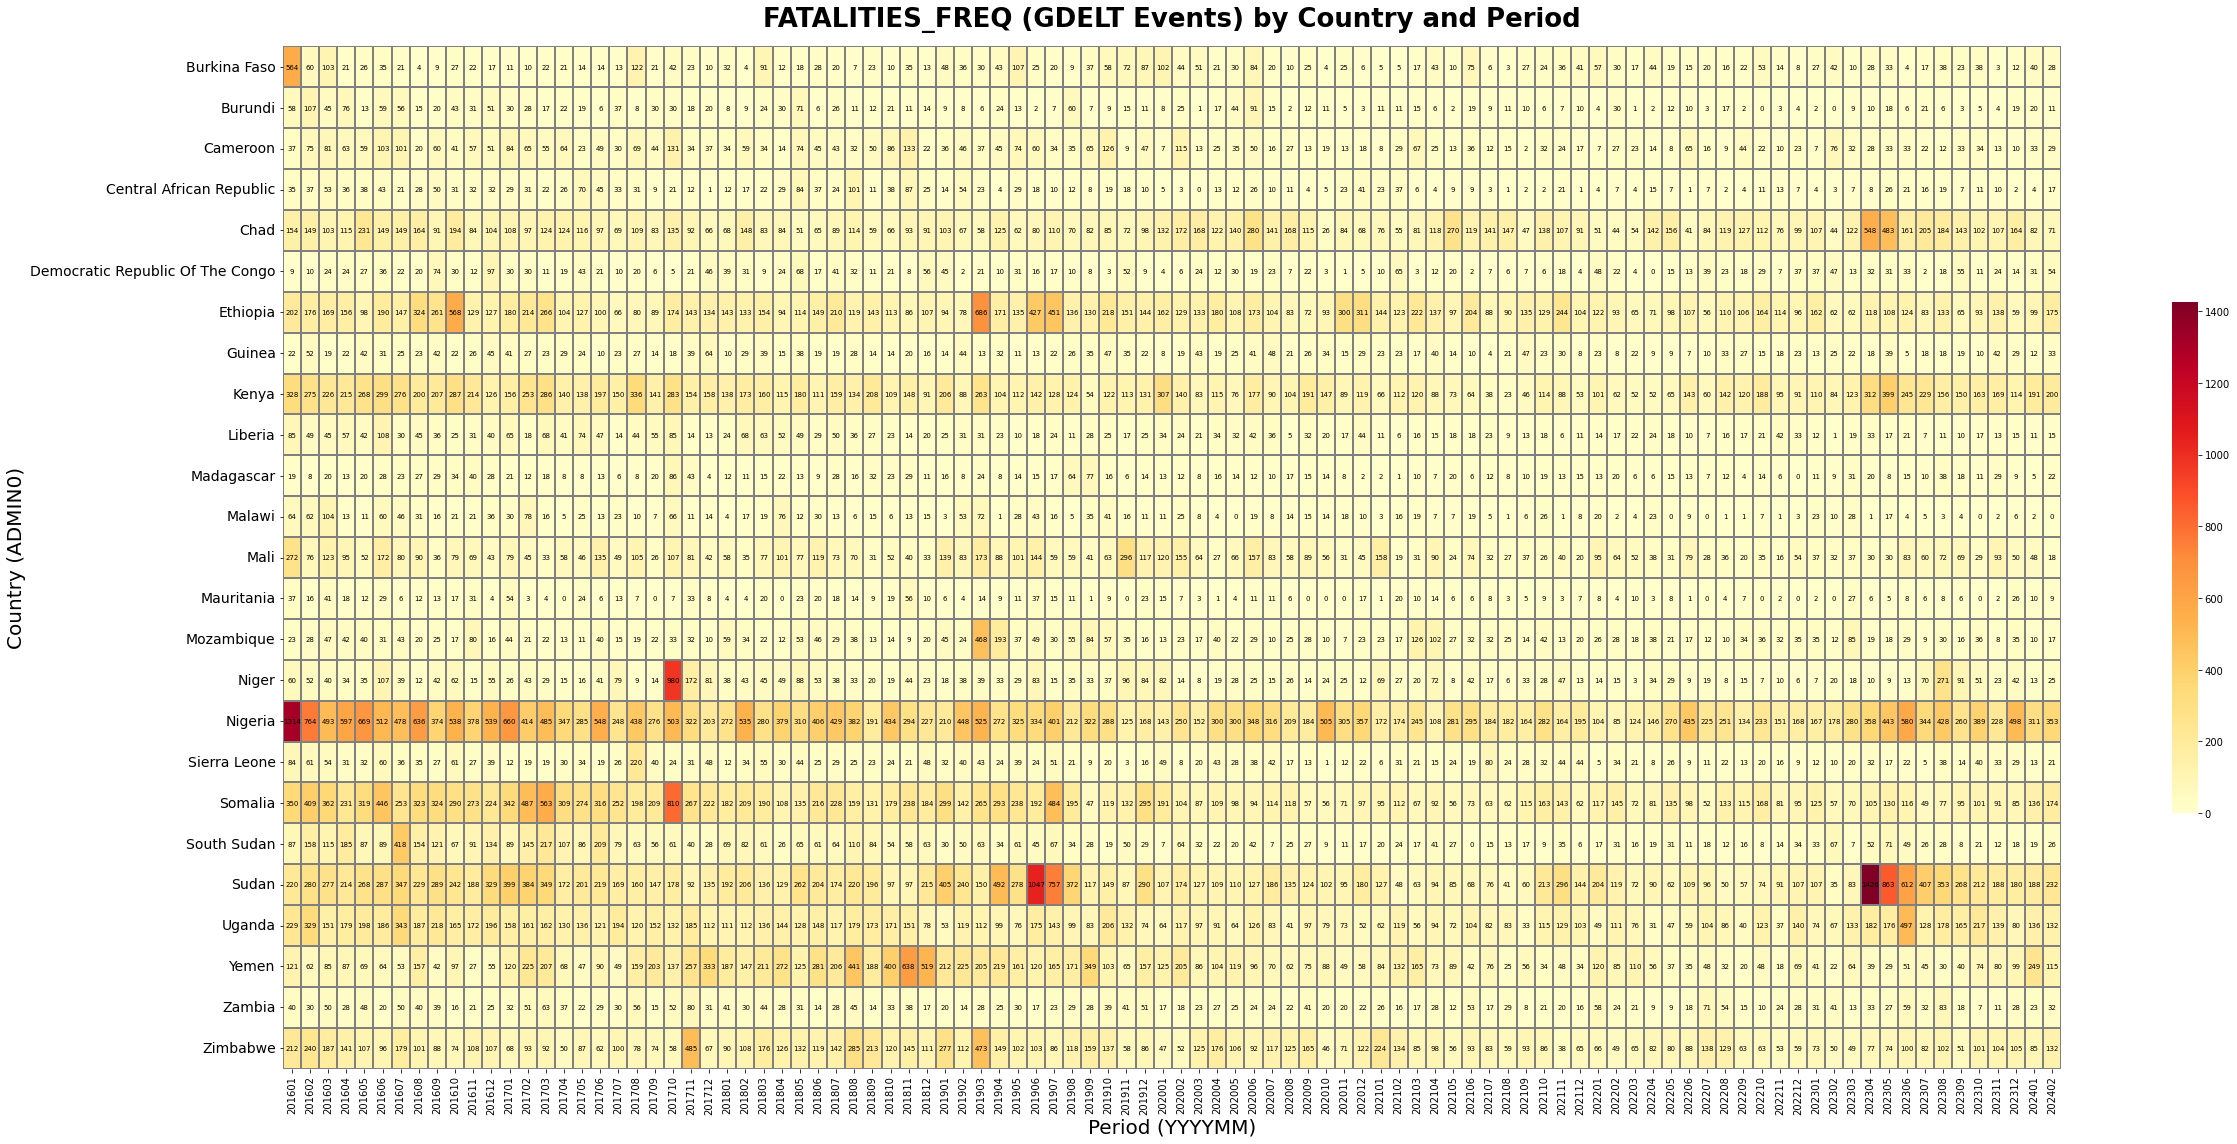
\includegraphics[width=\textwidth]{fatalities_freq.png}
    \caption{\textbf{S5: Fatalities frequency.} Distinct regional and temporal spikes correspond to localized crises with high reported fatalities.}
\end{figure}

\begin{figure}[H]
    \centering
    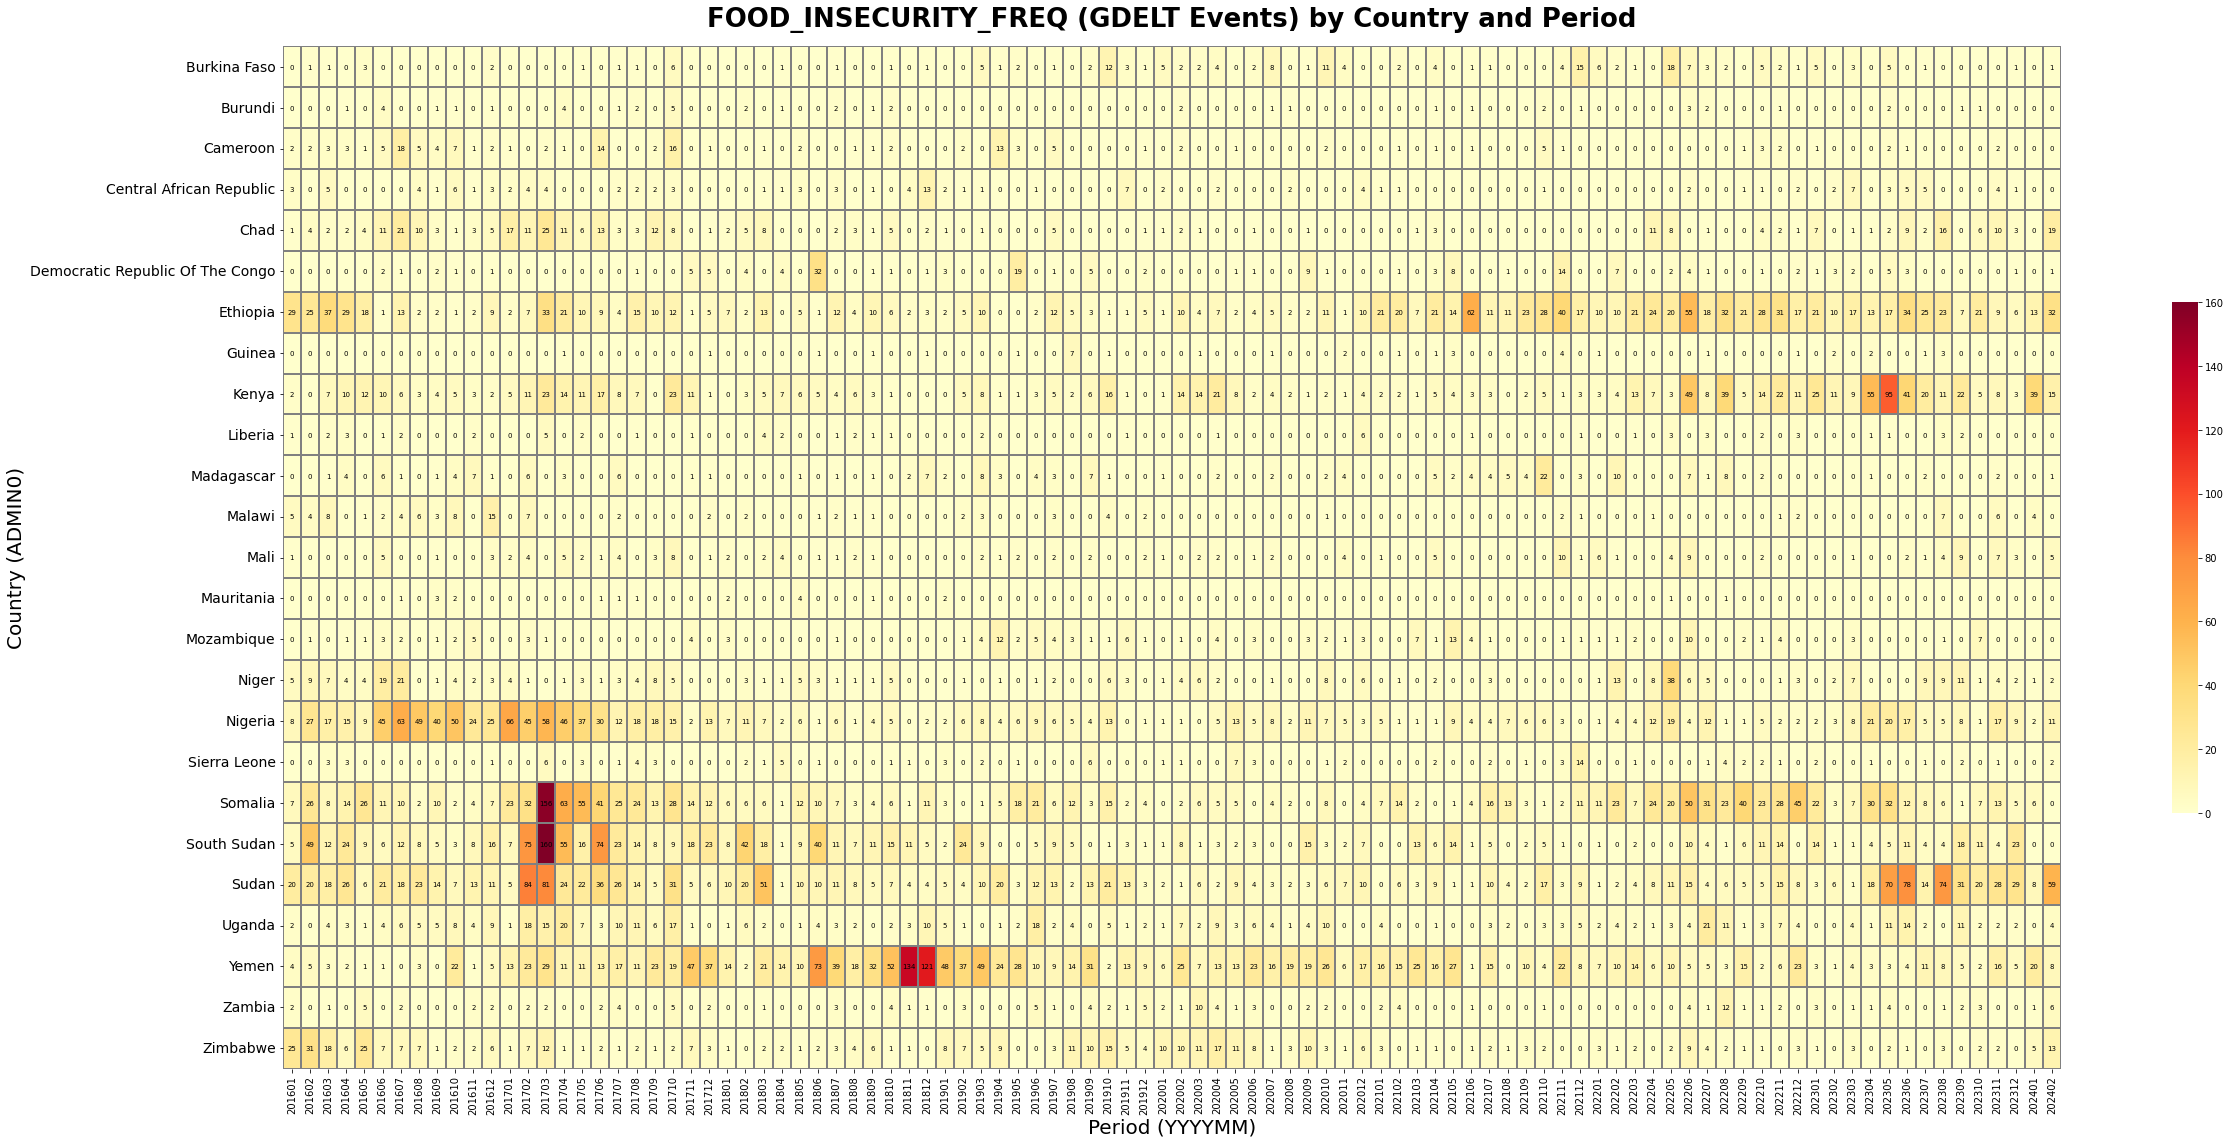
\includegraphics[width=\textwidth]{food_insecurity_freq.png}
    \caption{\textbf{S6: Food insecurity frequency.} Strong signal in crisis-affected regions and periods; highlights periods of acute need.}
\end{figure}

\begin{figure}[H]
    \centering
    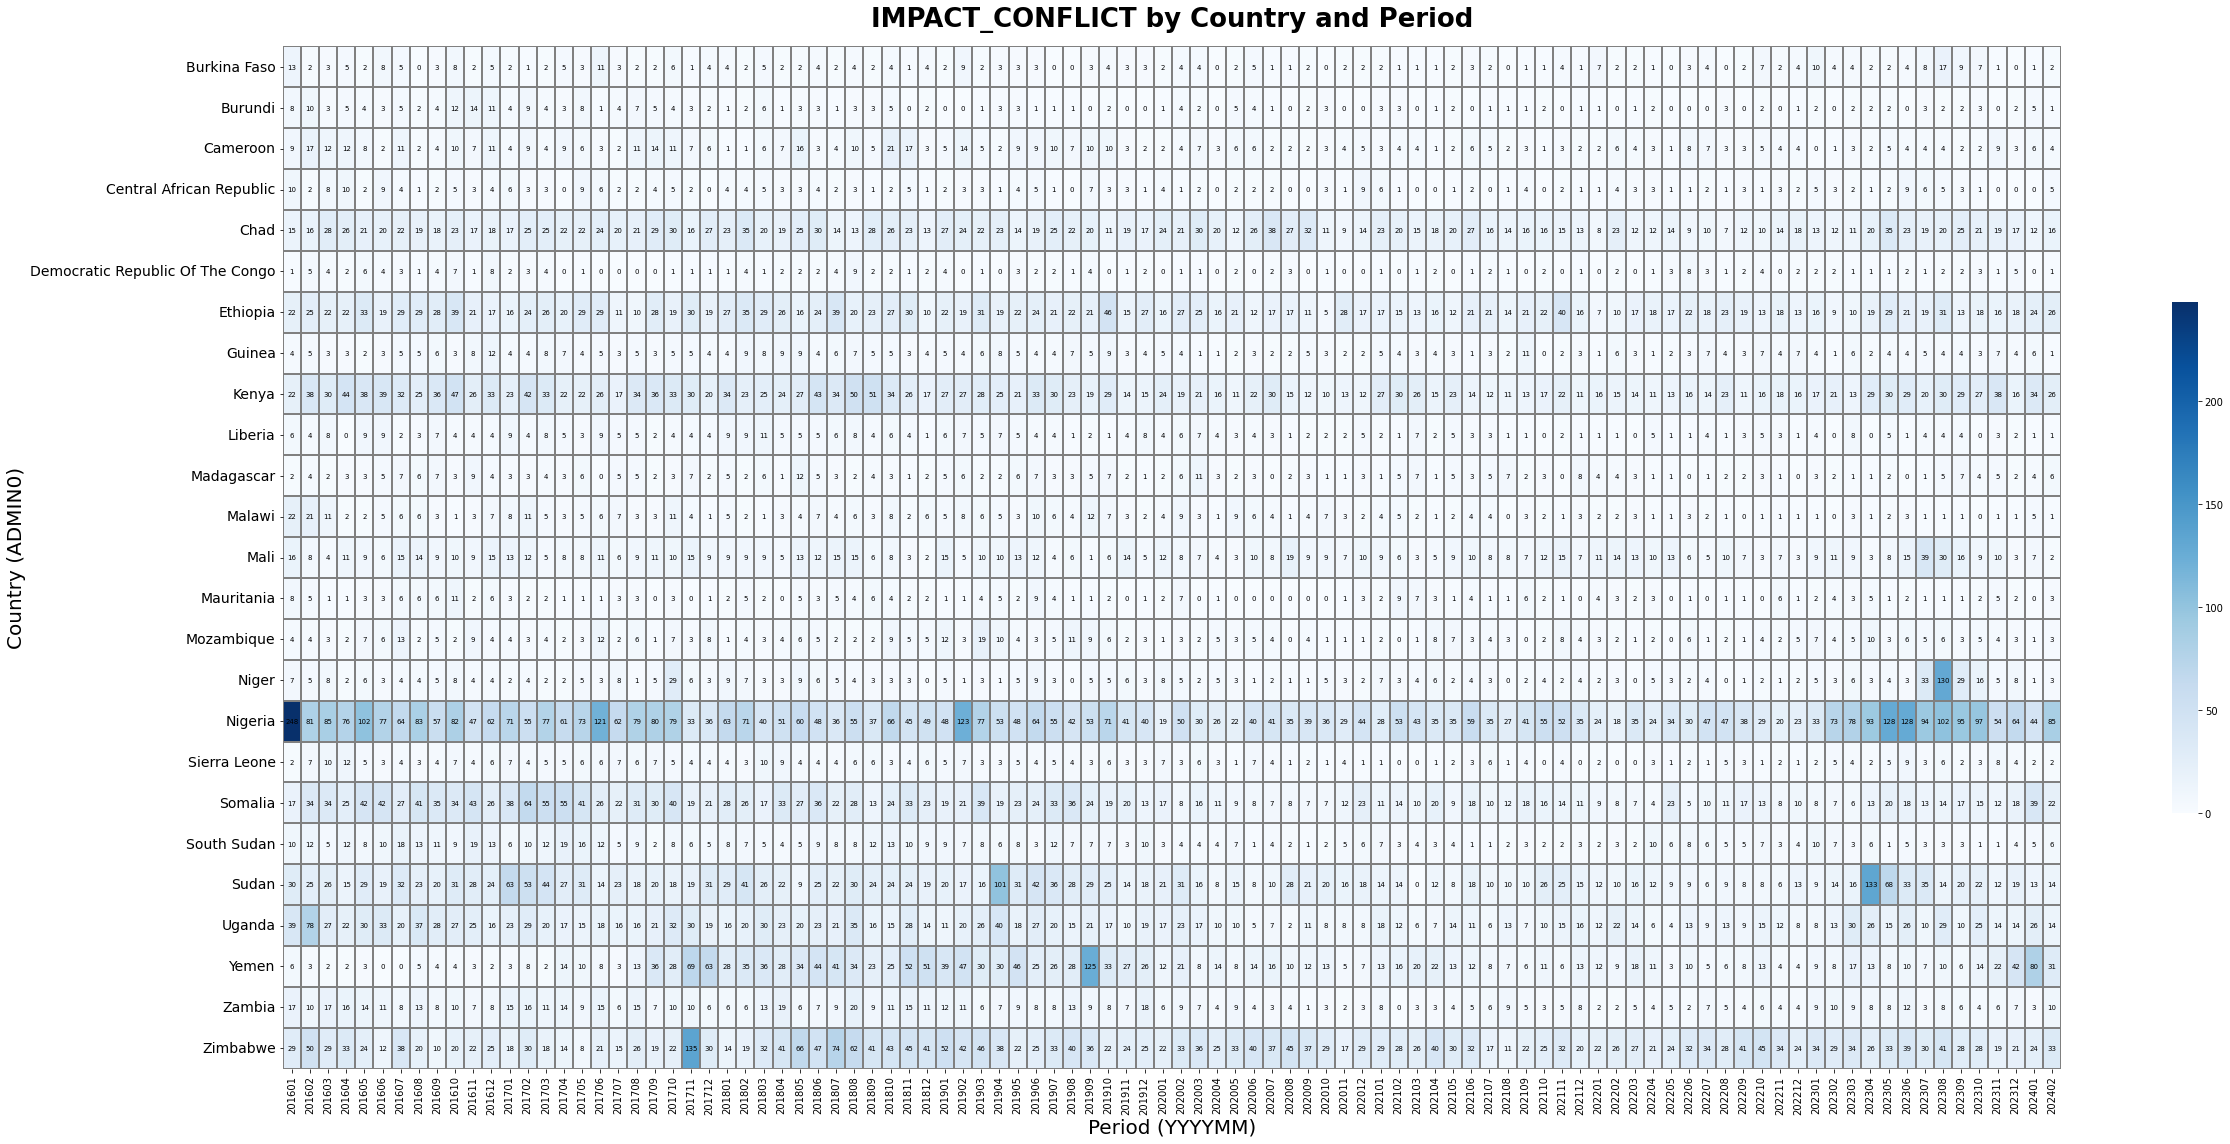
\includegraphics[width=\textwidth]{impact_conflict.png}
    \caption{\textbf{S7: Conflict impact mentions.} Marked temporal variation and regional clustering of conflict-related reporting.}
\end{figure}

\begin{figure}[H]
    \centering
    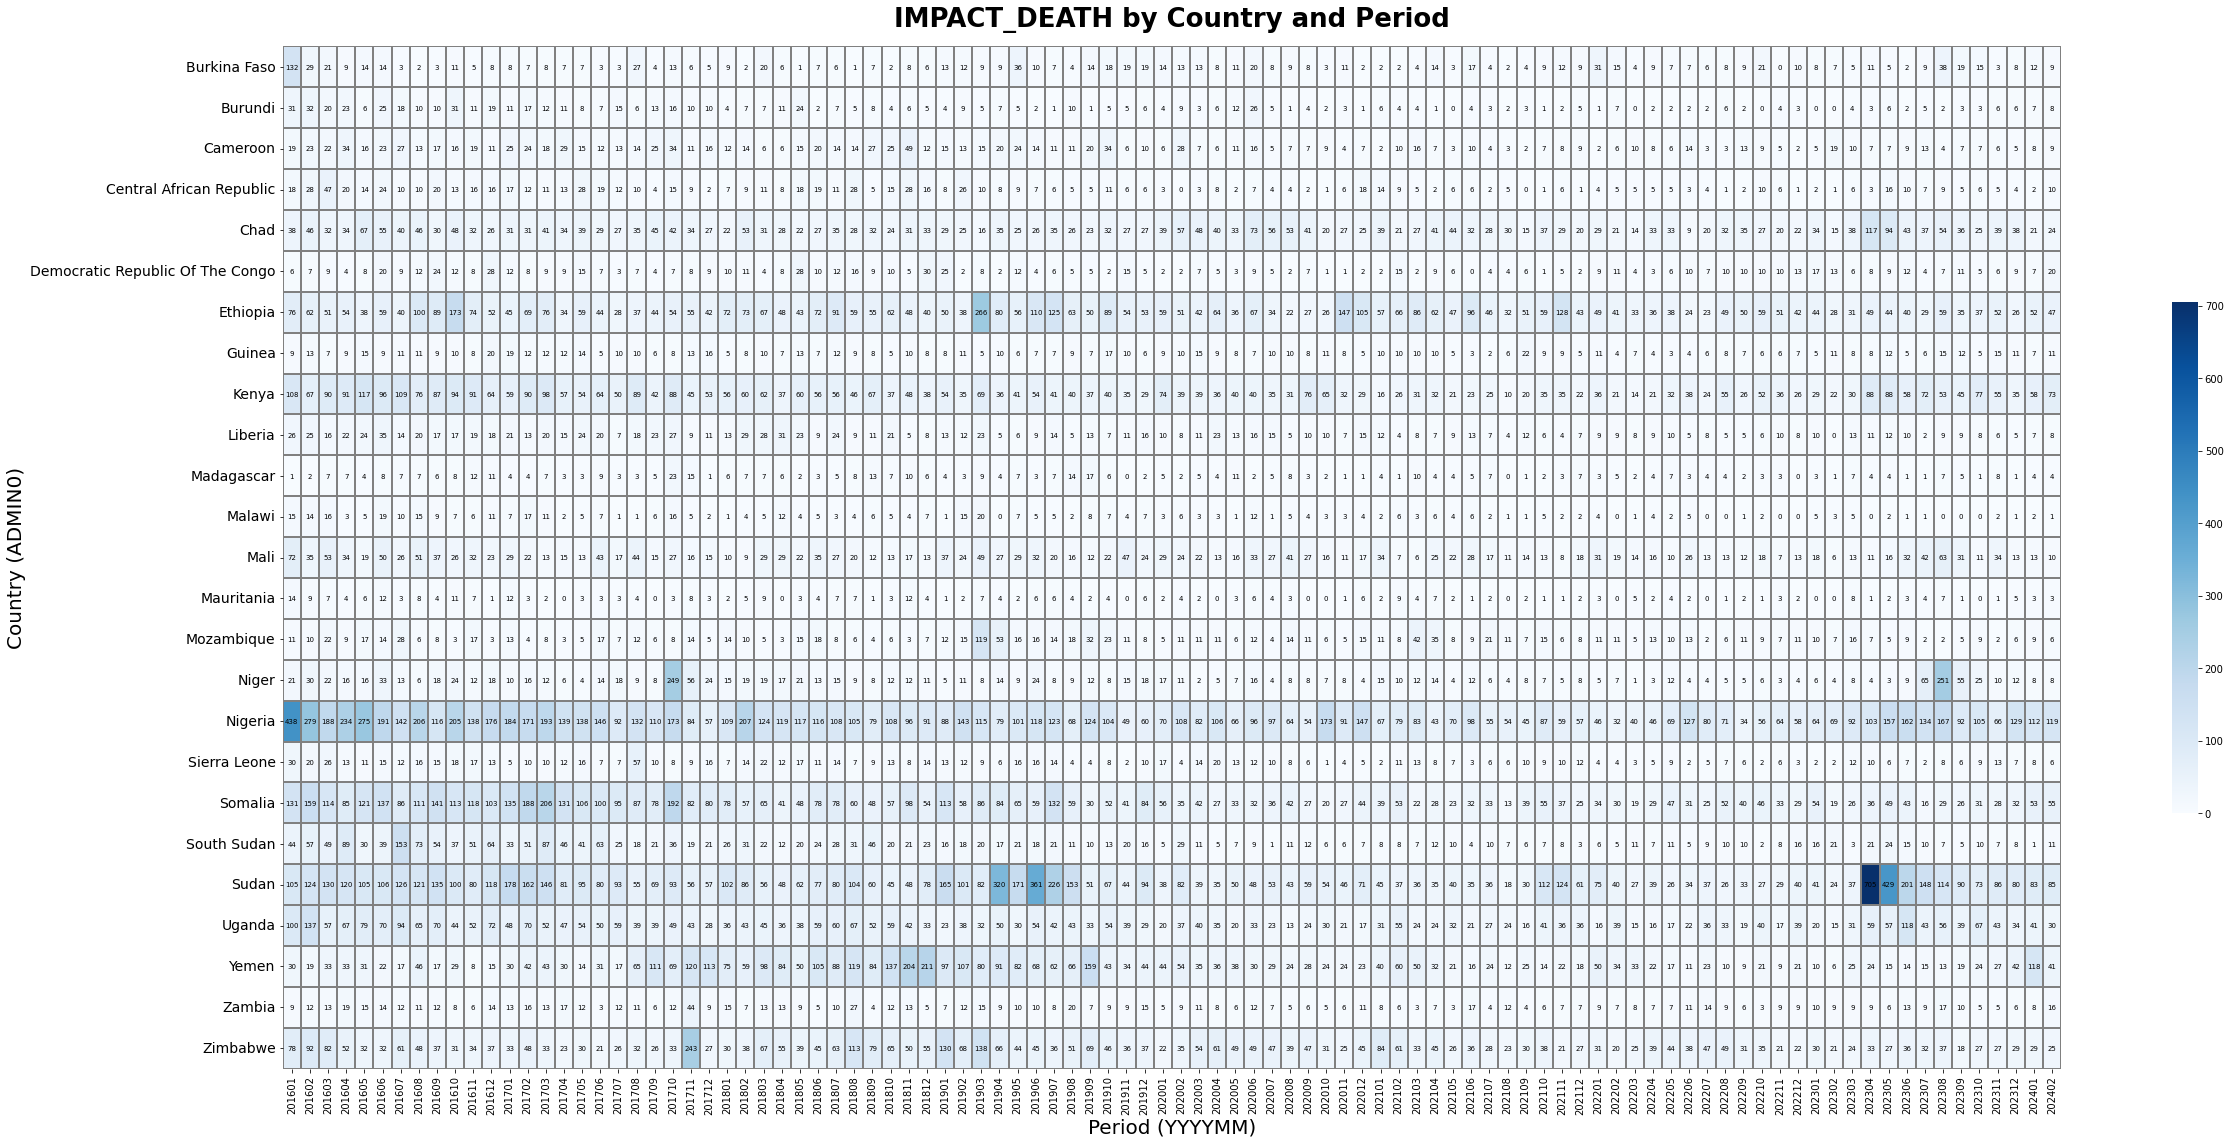
\includegraphics[width=\textwidth]{impact_death.png}
    \caption{\textbf{S8: Death impact mentions.} Spikes align with regions and periods experiencing elevated mortality.}
\end{figure}

\begin{figure}[H]
    \centering
    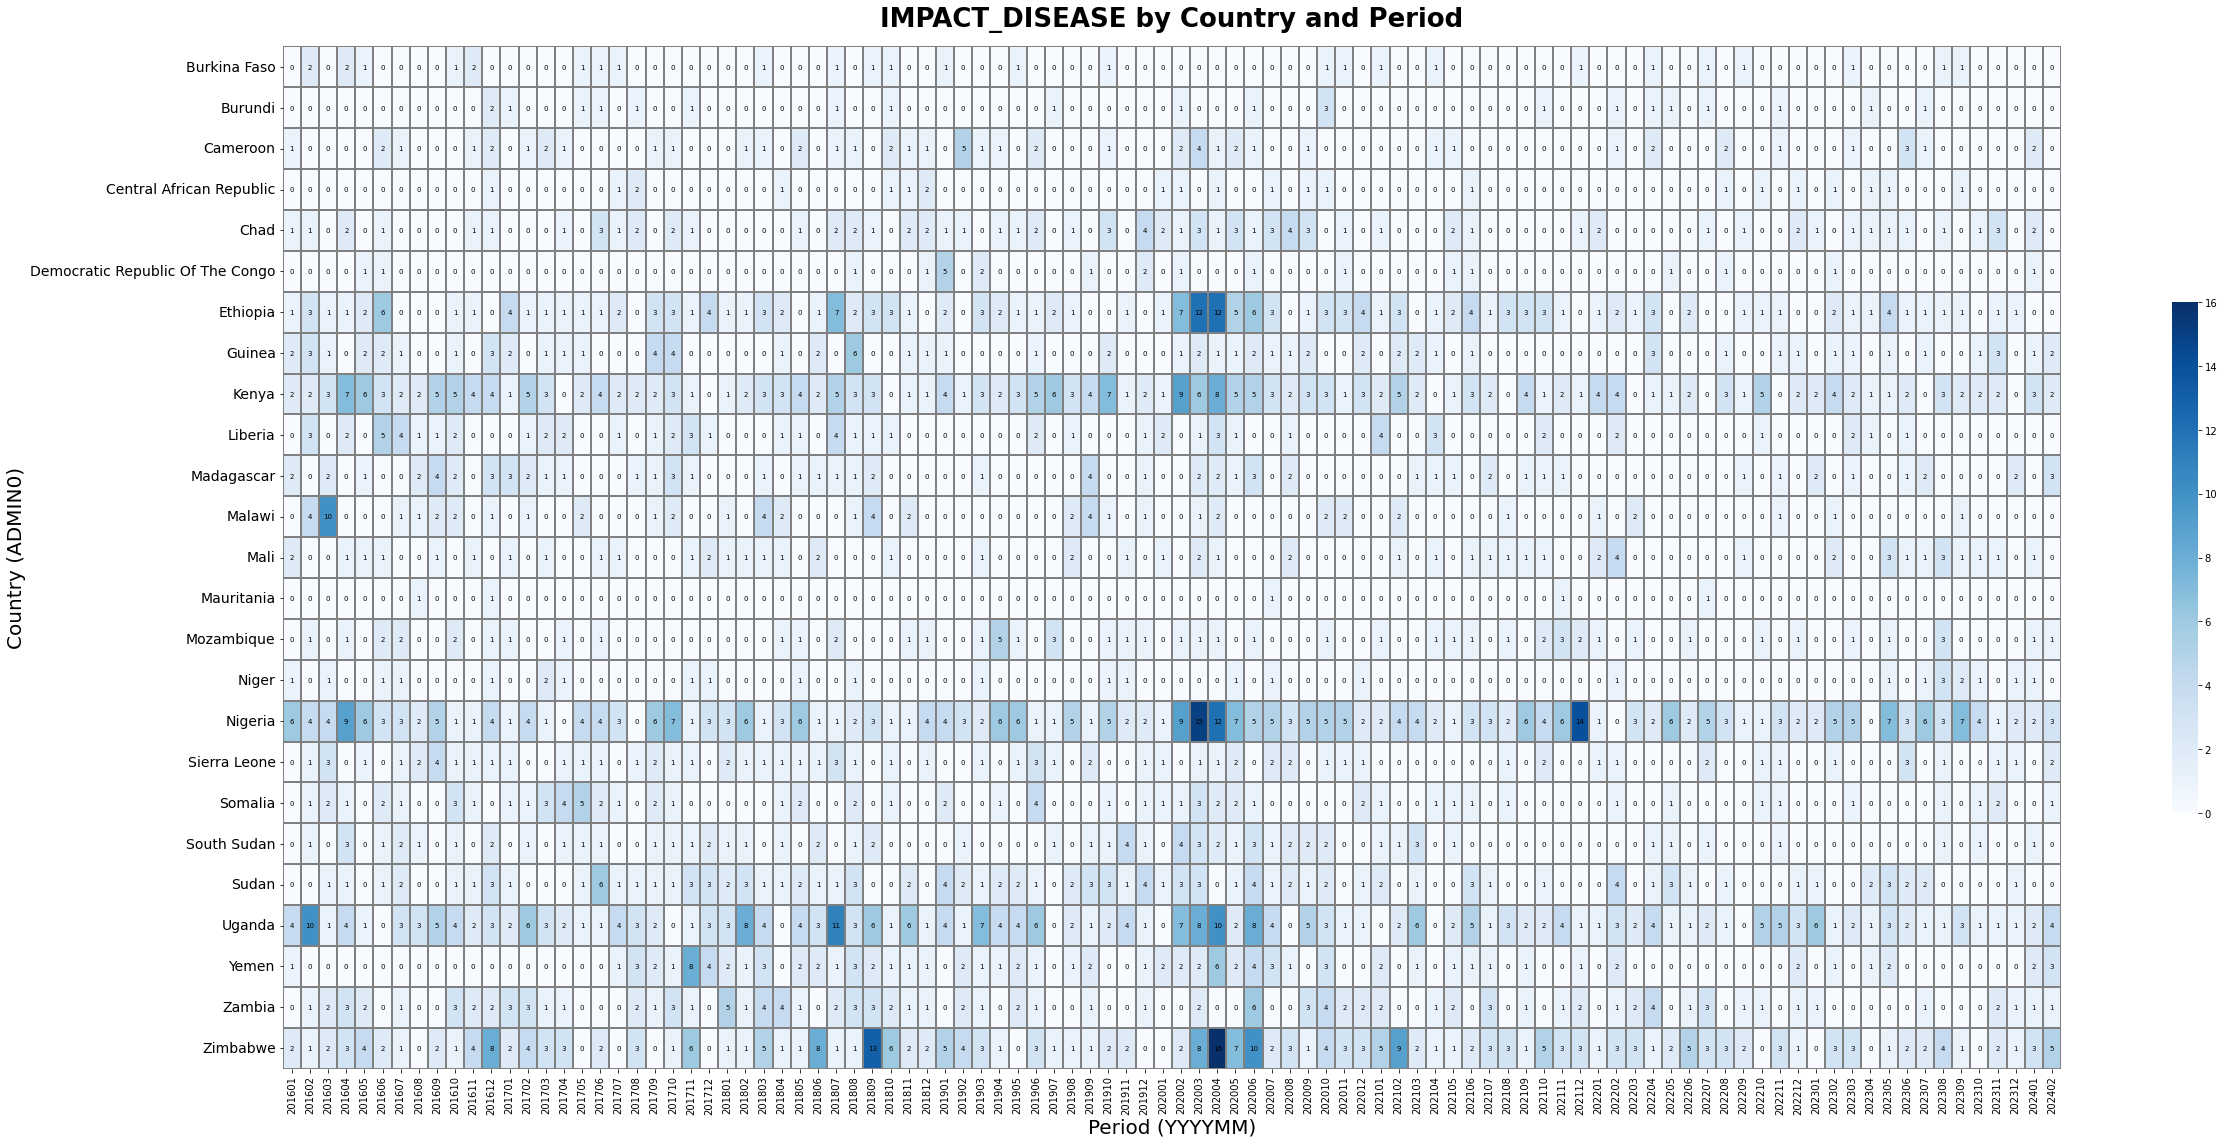
\includegraphics[width=\textwidth]{impact_disease.png}
    \caption{\textbf{S9: Disease impact mentions.} Variable signal, with distinct peaks reflecting outbreak reporting.}
\end{figure}

\begin{figure}[H]
    \centering
    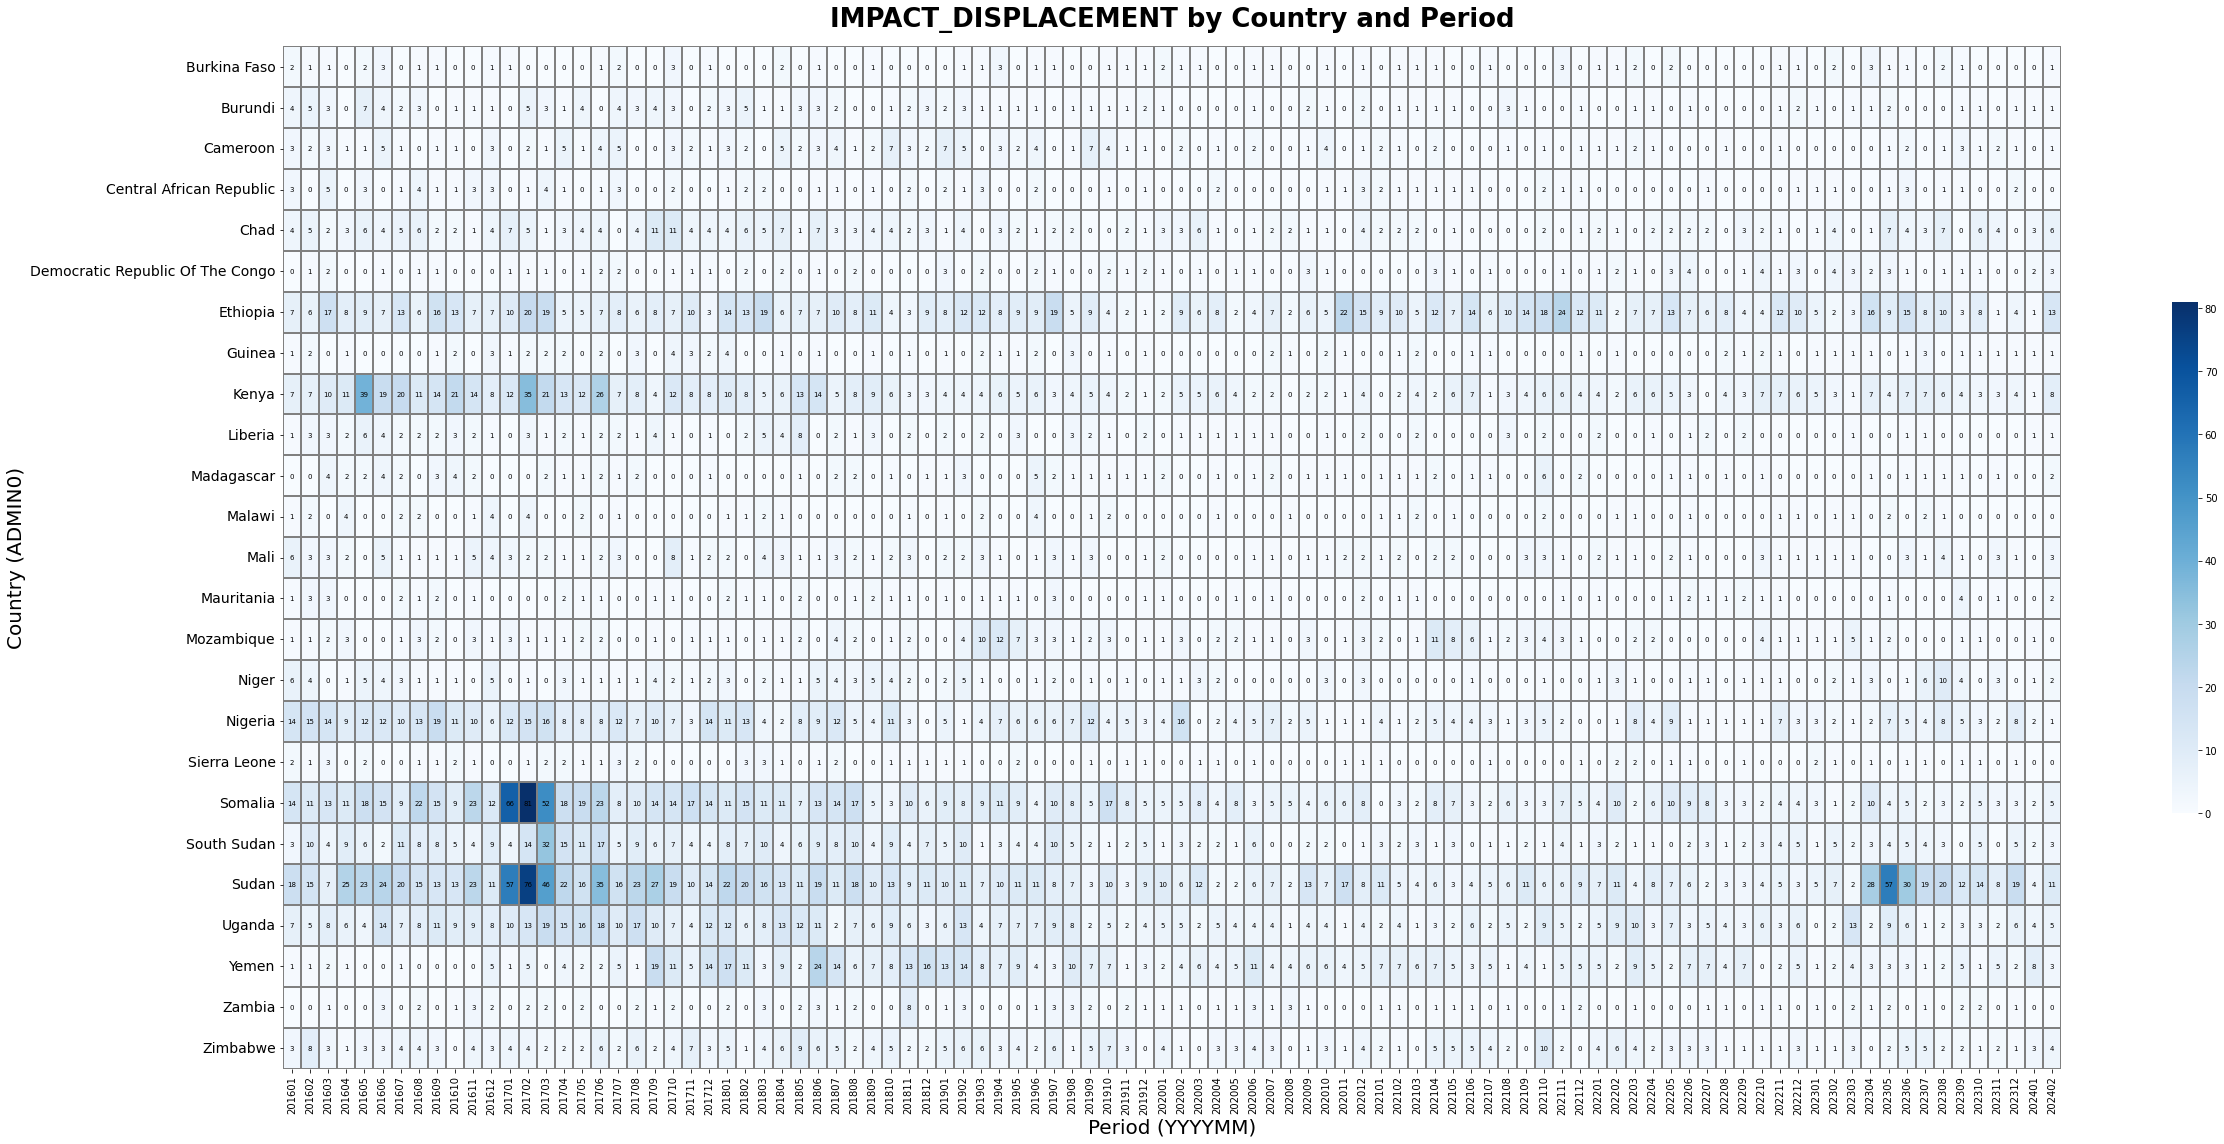
\includegraphics[width=\textwidth]{impact_displacement.png}
    \caption{\textbf{S10: Displacement impact mentions.} Concentrated spikes correspond to periods of mass displacement events.}
\end{figure}

\begin{figure}[H]
    \centering
    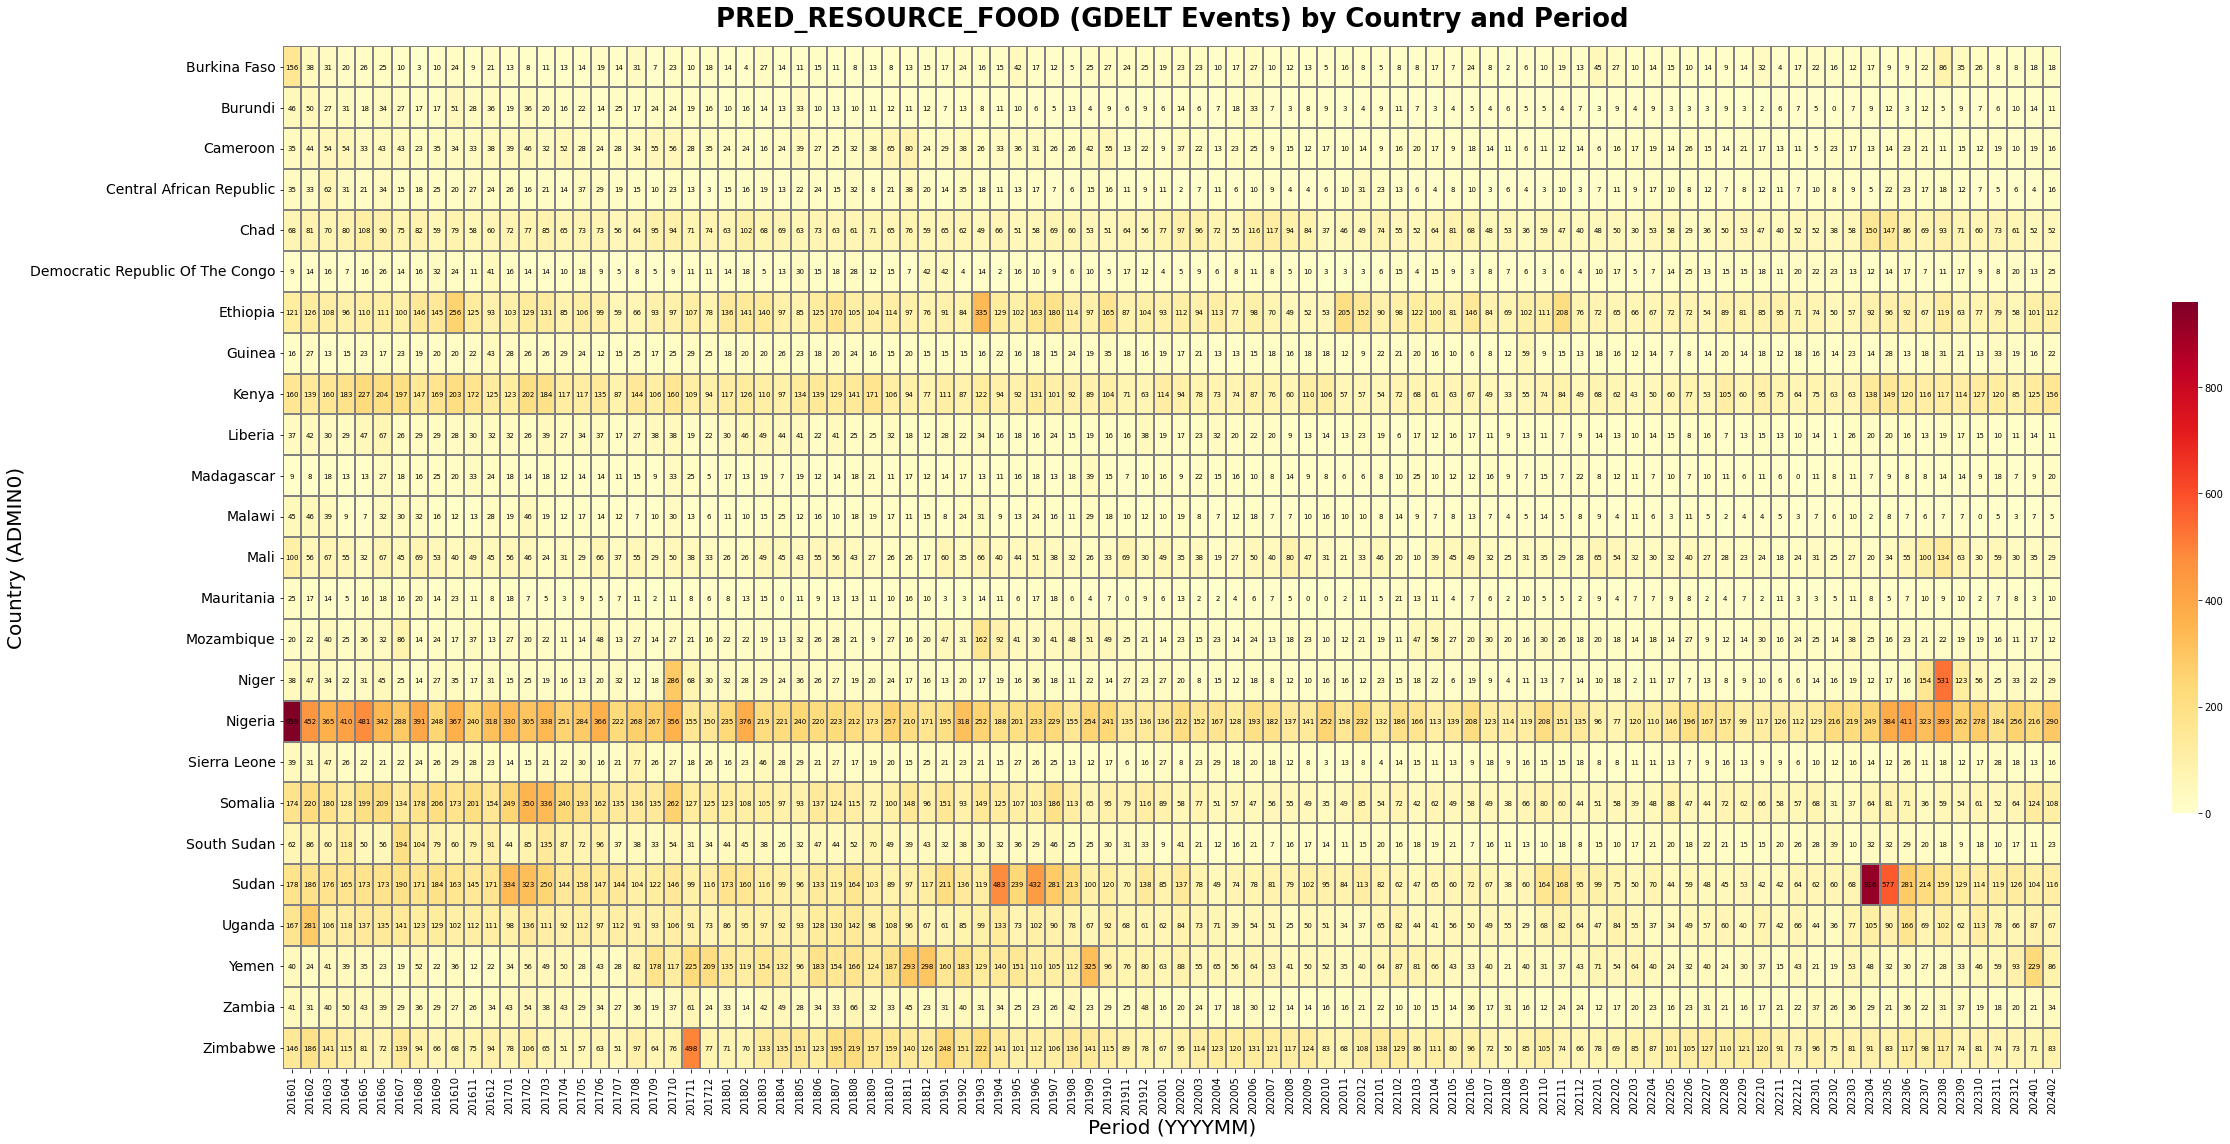
\includegraphics[width=\textwidth]{pred_resources_food.png}
    \caption{\textbf{S11: Predicted need for food aid.} Strong regional clustering in crisis periods.}
\end{figure}

\begin{figure}[H]
    \centering
    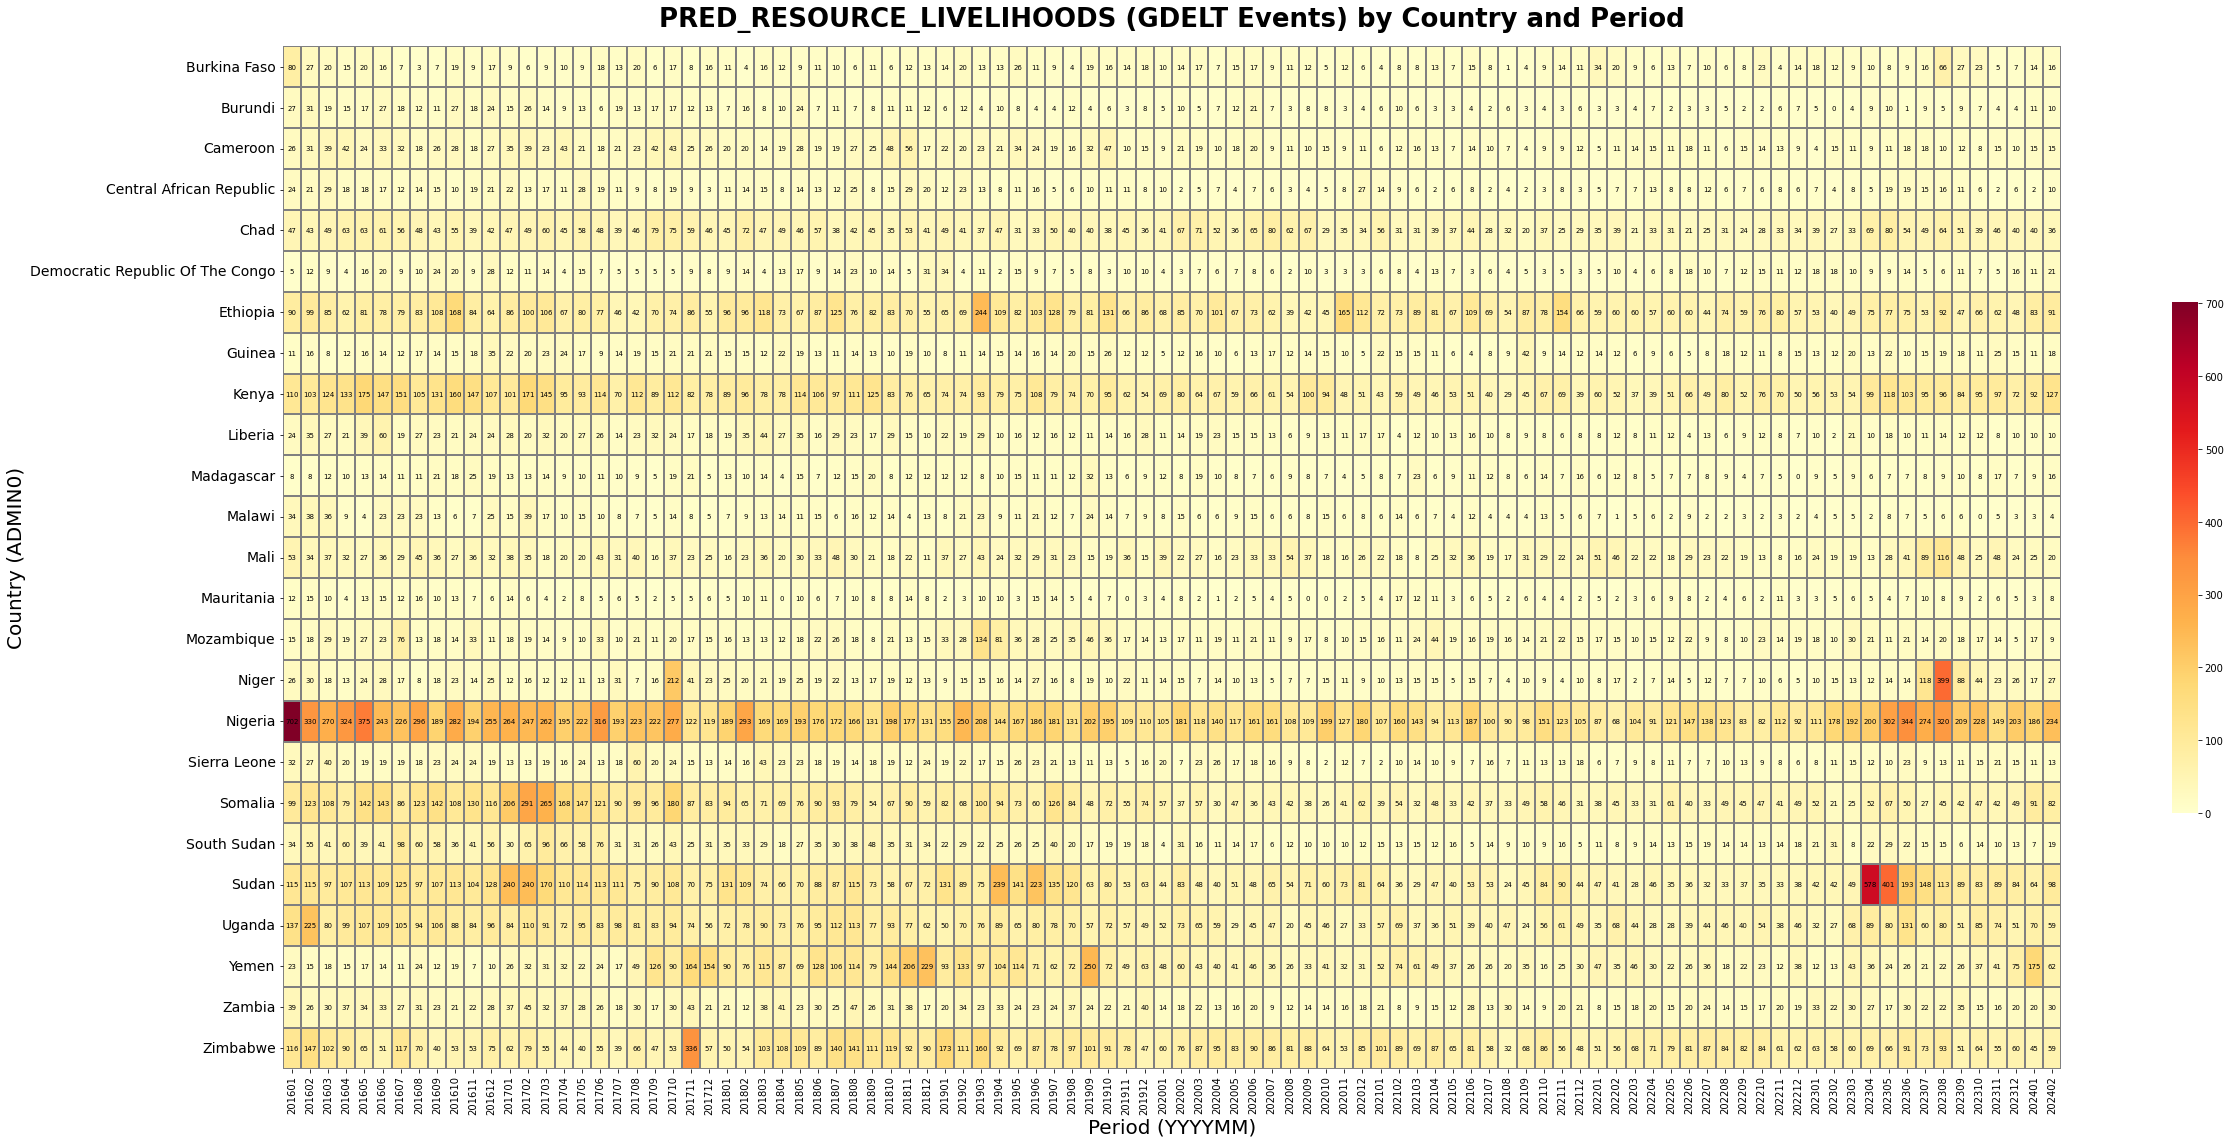
\includegraphics[width=\textwidth]{pred_resources_livelihood.png}
    \caption{\textbf{S12: Predicted need for livelihood support.} Moderate variation with localized regional peaks.}
\end{figure}

\begin{figure}[H]
    \centering
    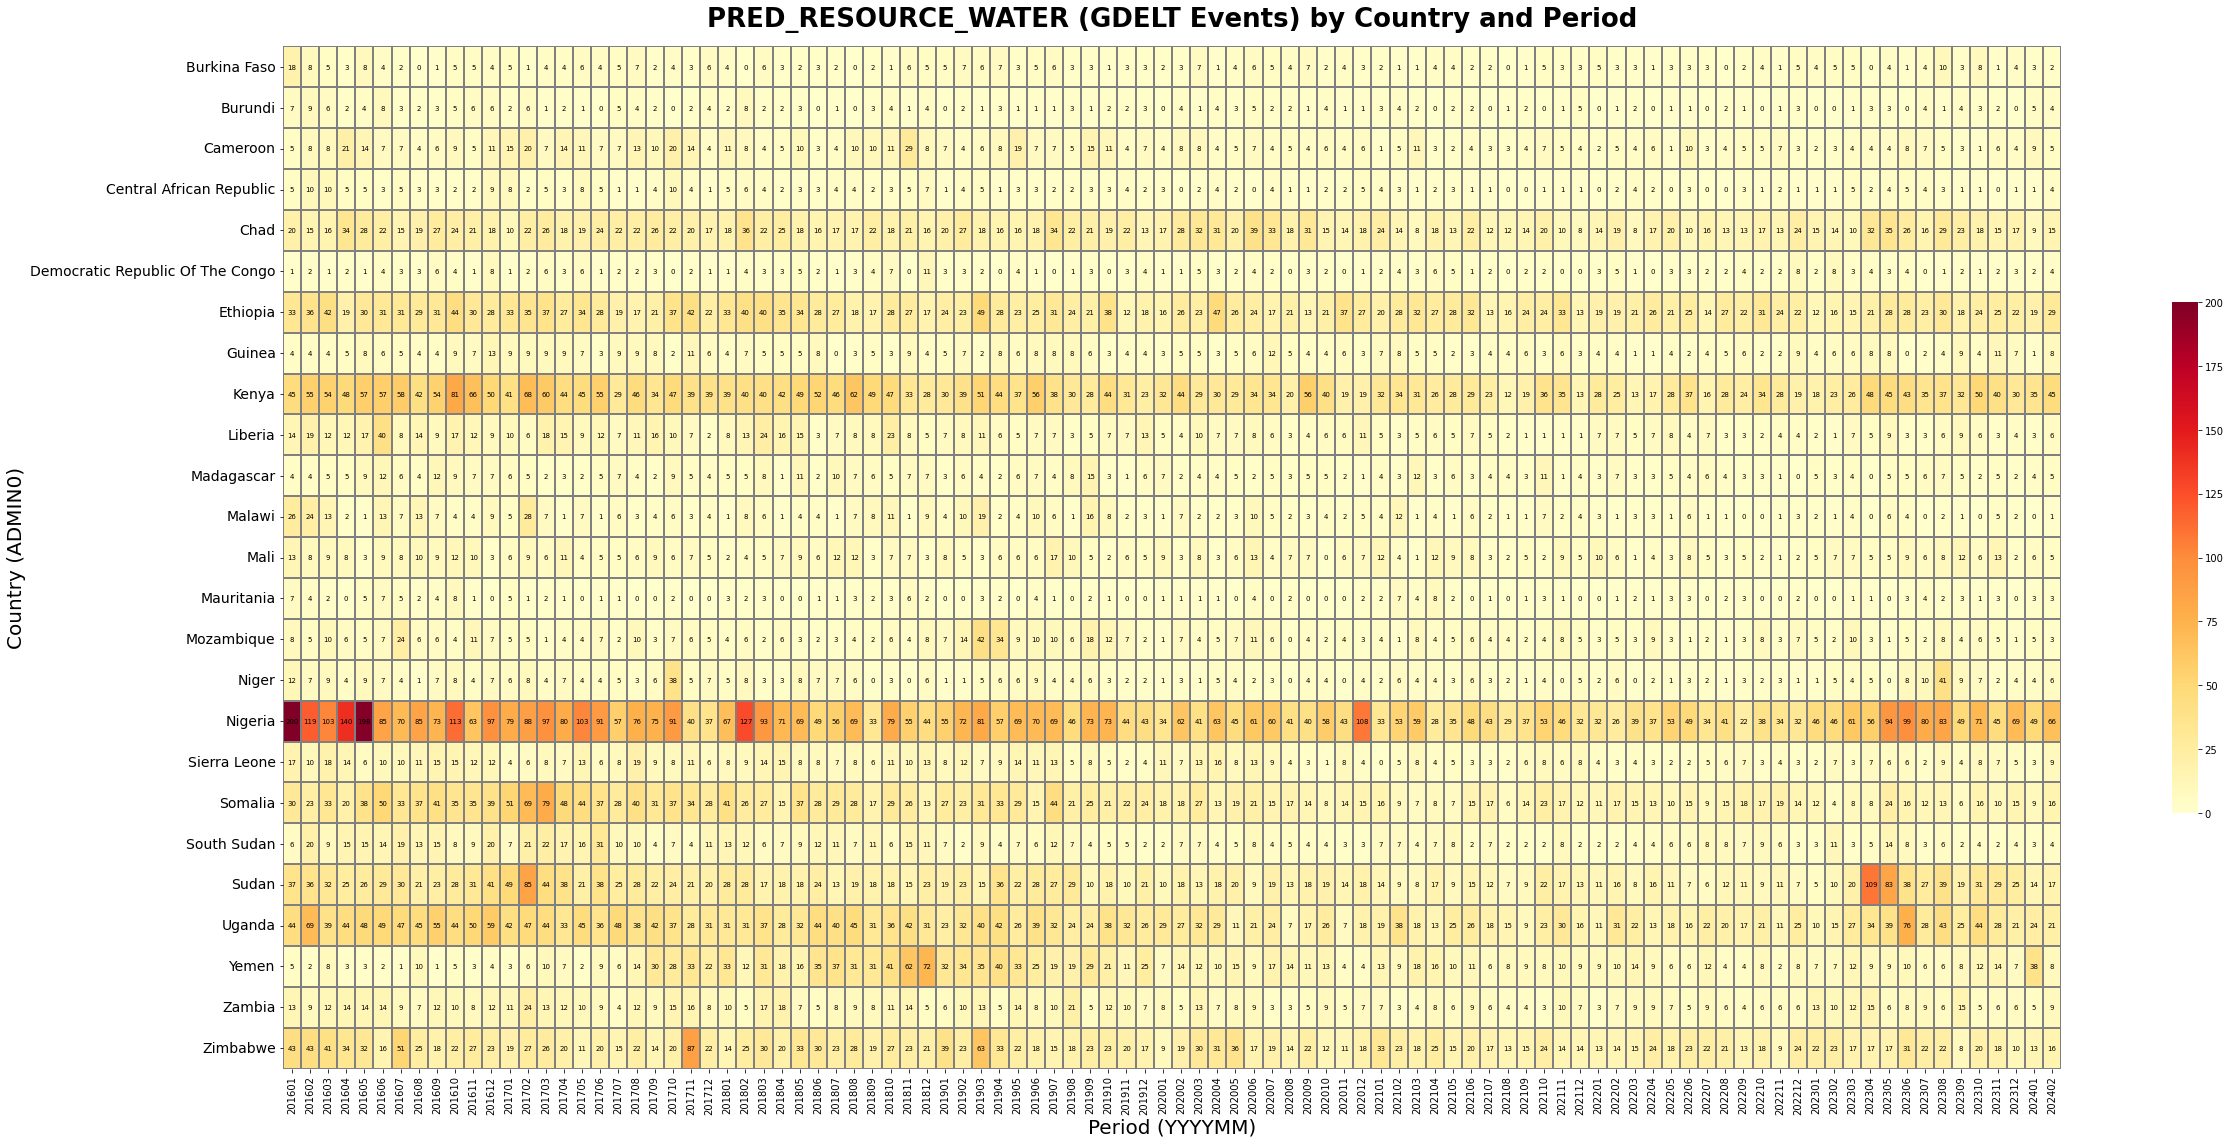
\includegraphics[width=\textwidth]{pred_resources_water.png}
    \caption{\textbf{S13: Predicted need for water aid.} Scattered peaks highlight periods of reported water insecurity.}
\end{figure}

\begin{figure}[H]
    \centering
    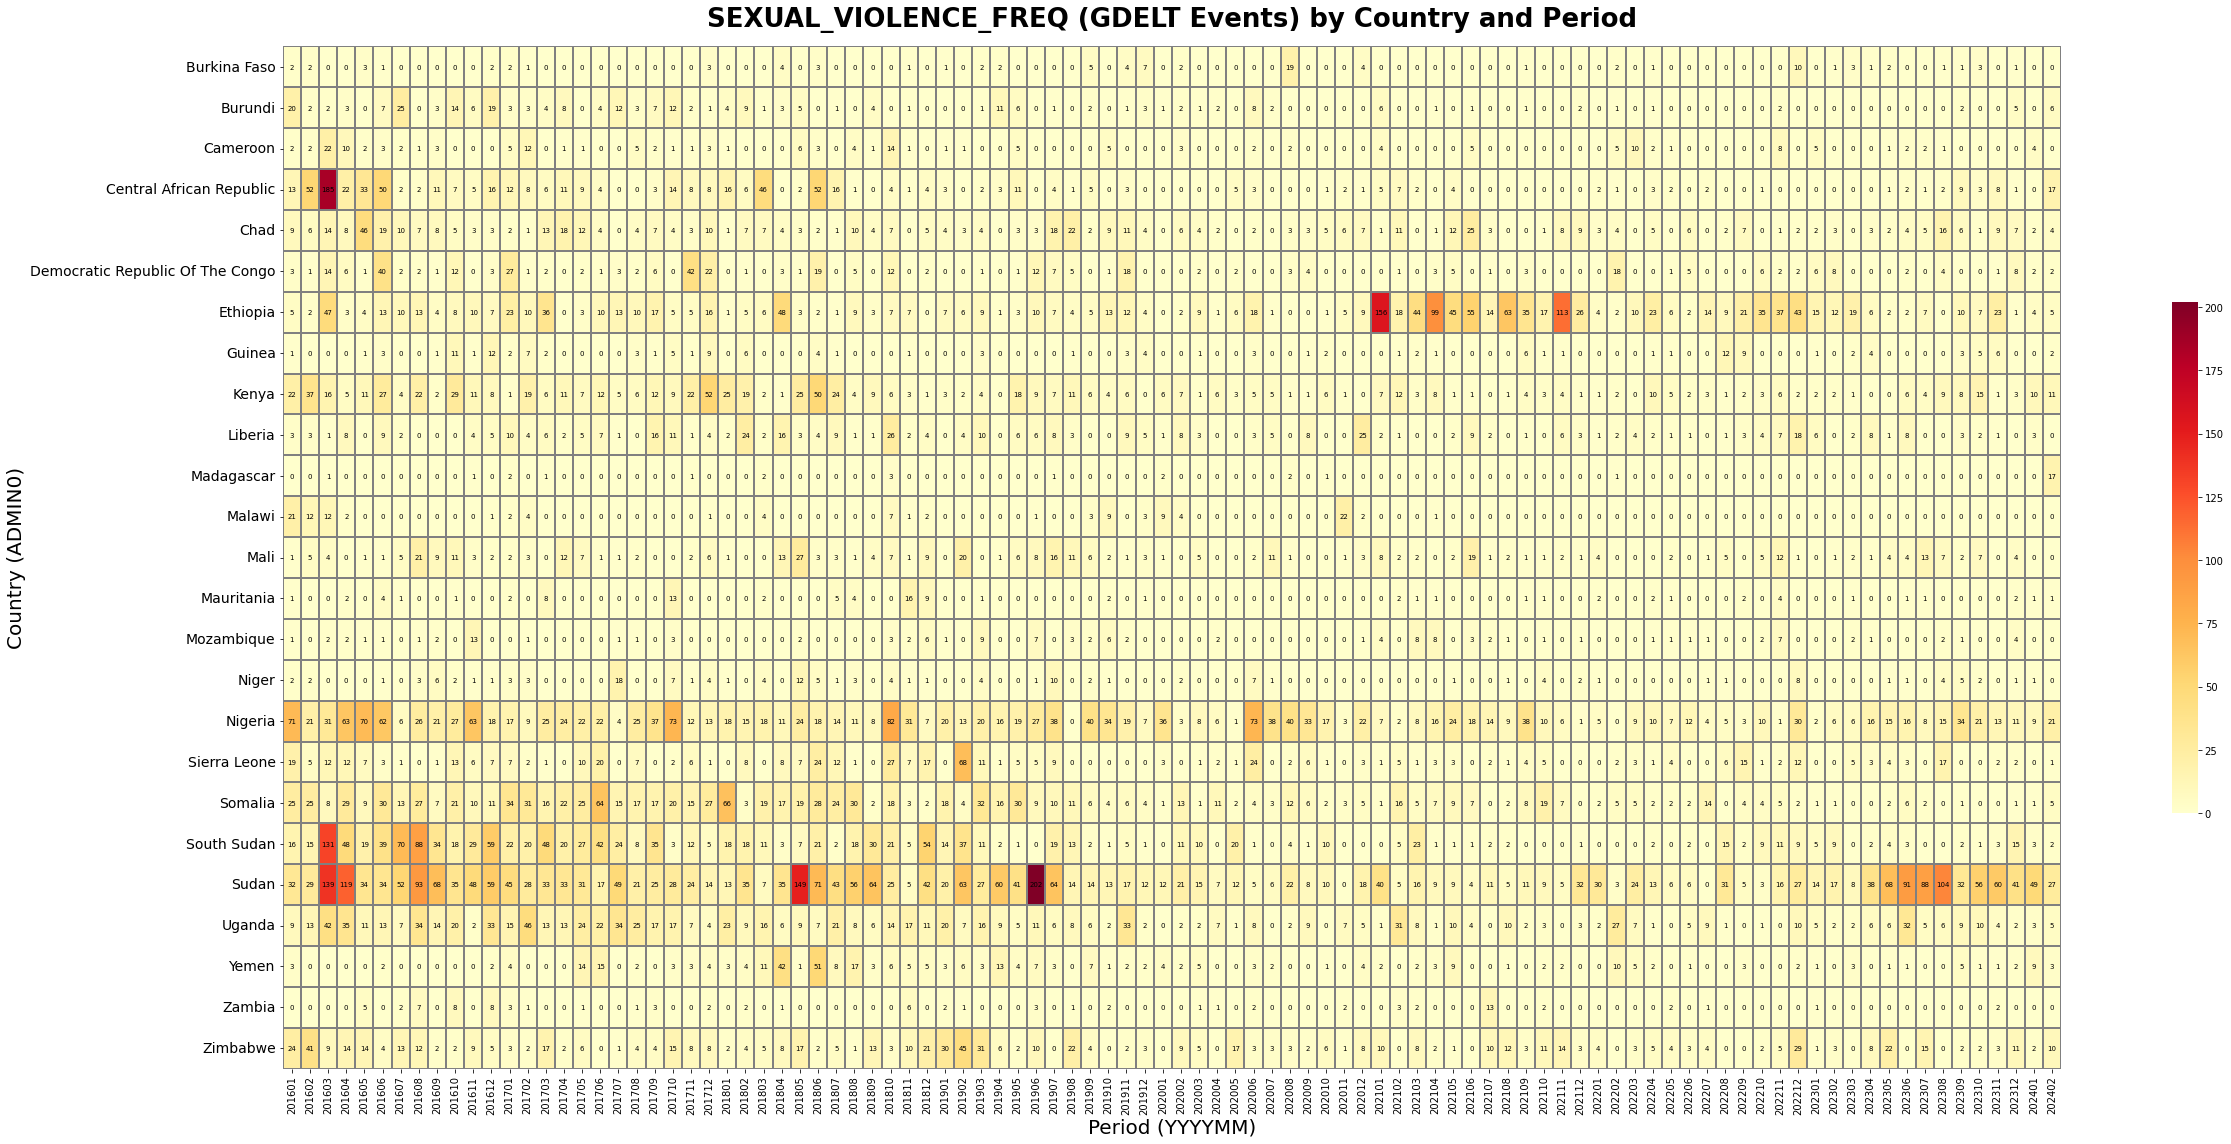
\includegraphics[width=\textwidth]{sexual_violence_freq.png}
    \caption{\textbf{S14: Sexual violence frequency.} Rare but highly localized signals, often reflecting reporting constraints.}
\end{figure}

\begin{figure}[H]
    \centering
    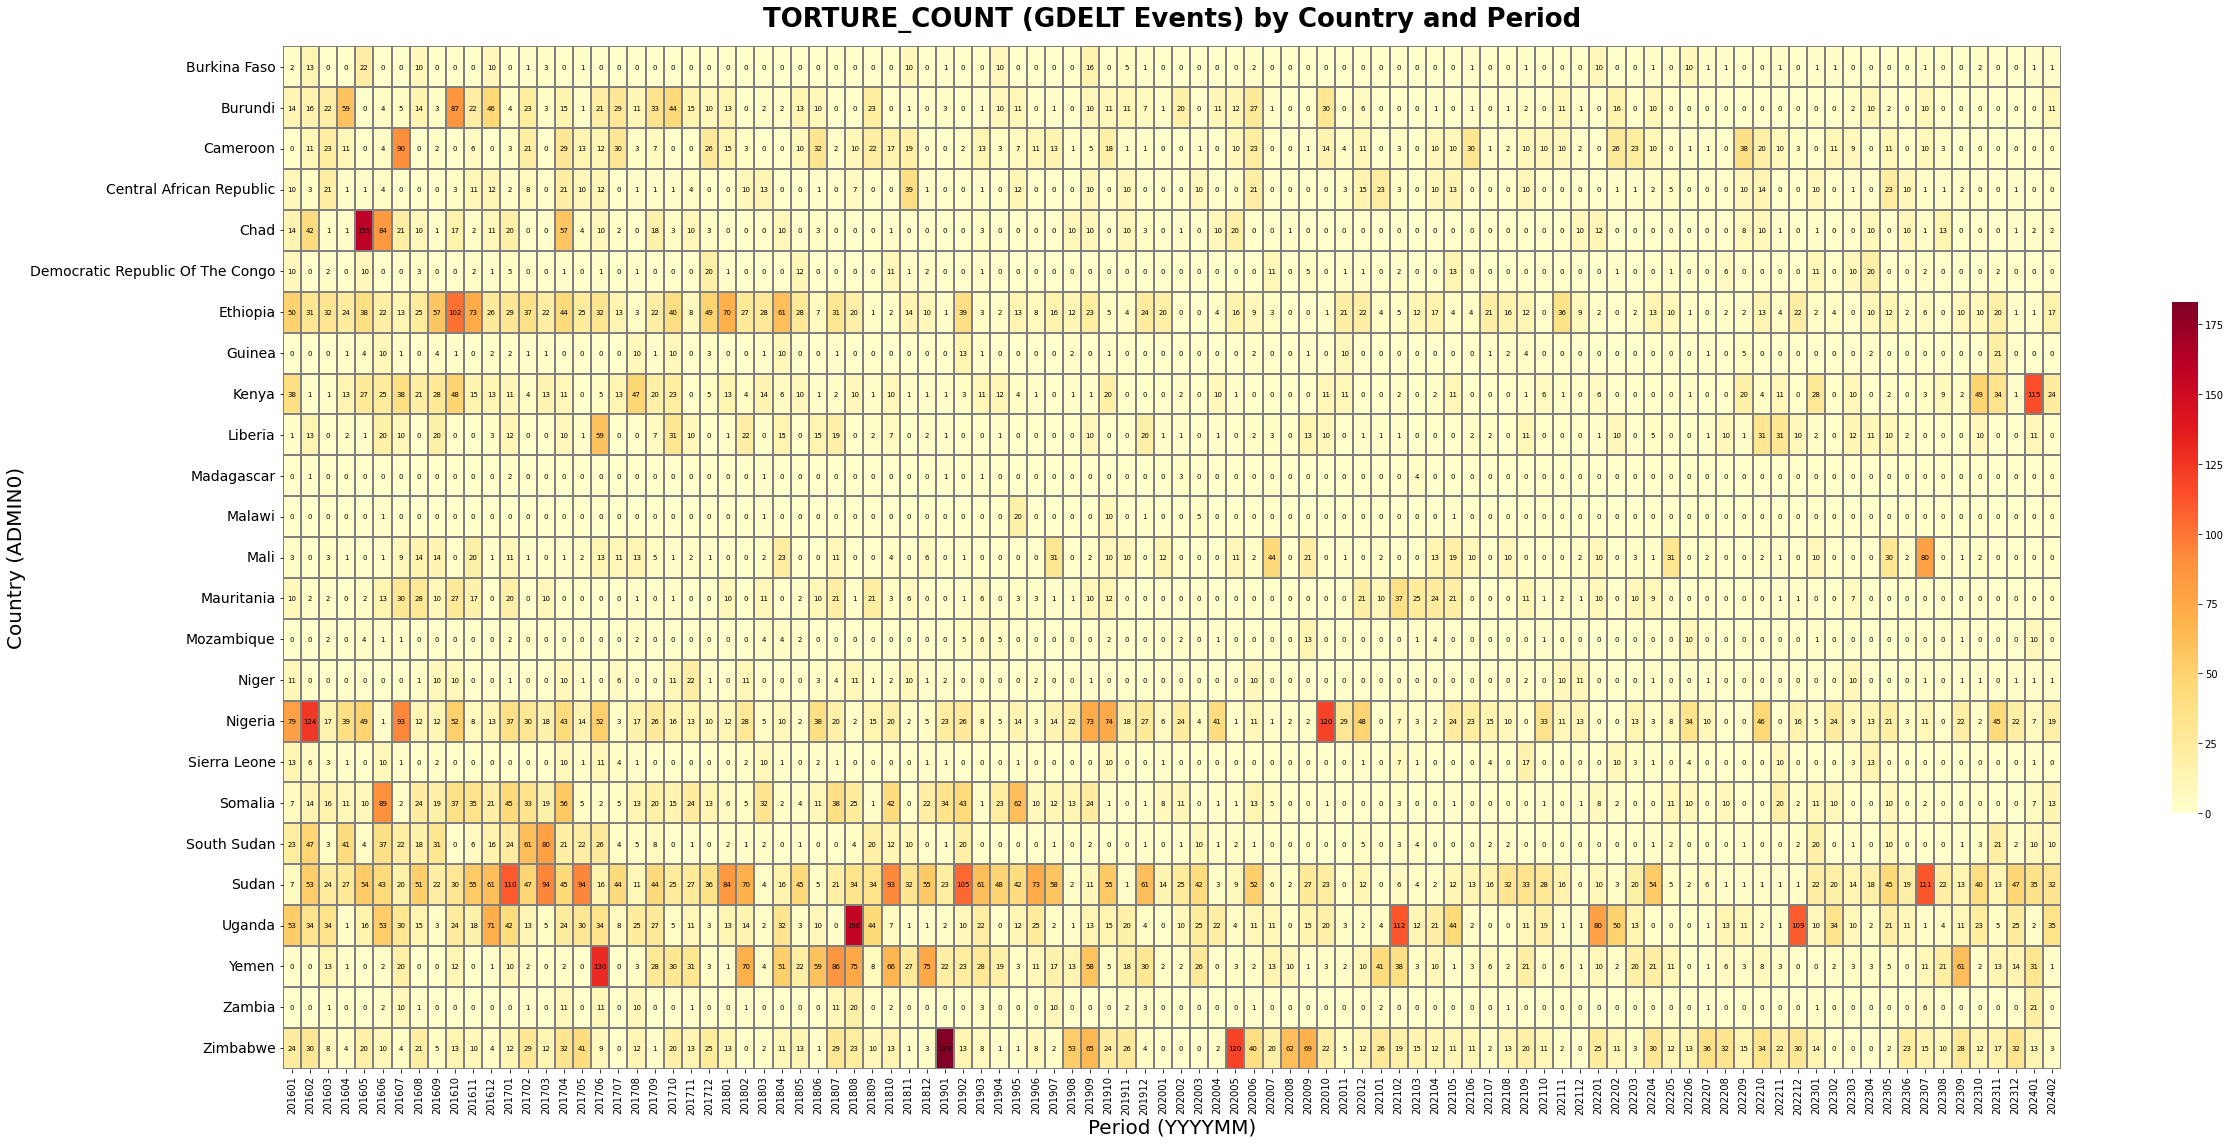
\includegraphics[width=\textwidth]{torture_count.png}
    \caption{\textbf{S15: Torture event counts.} Count metric reveals clear clustering in specific countries and periods.}
\end{figure}

\begin{figure}[H]
    \centering
    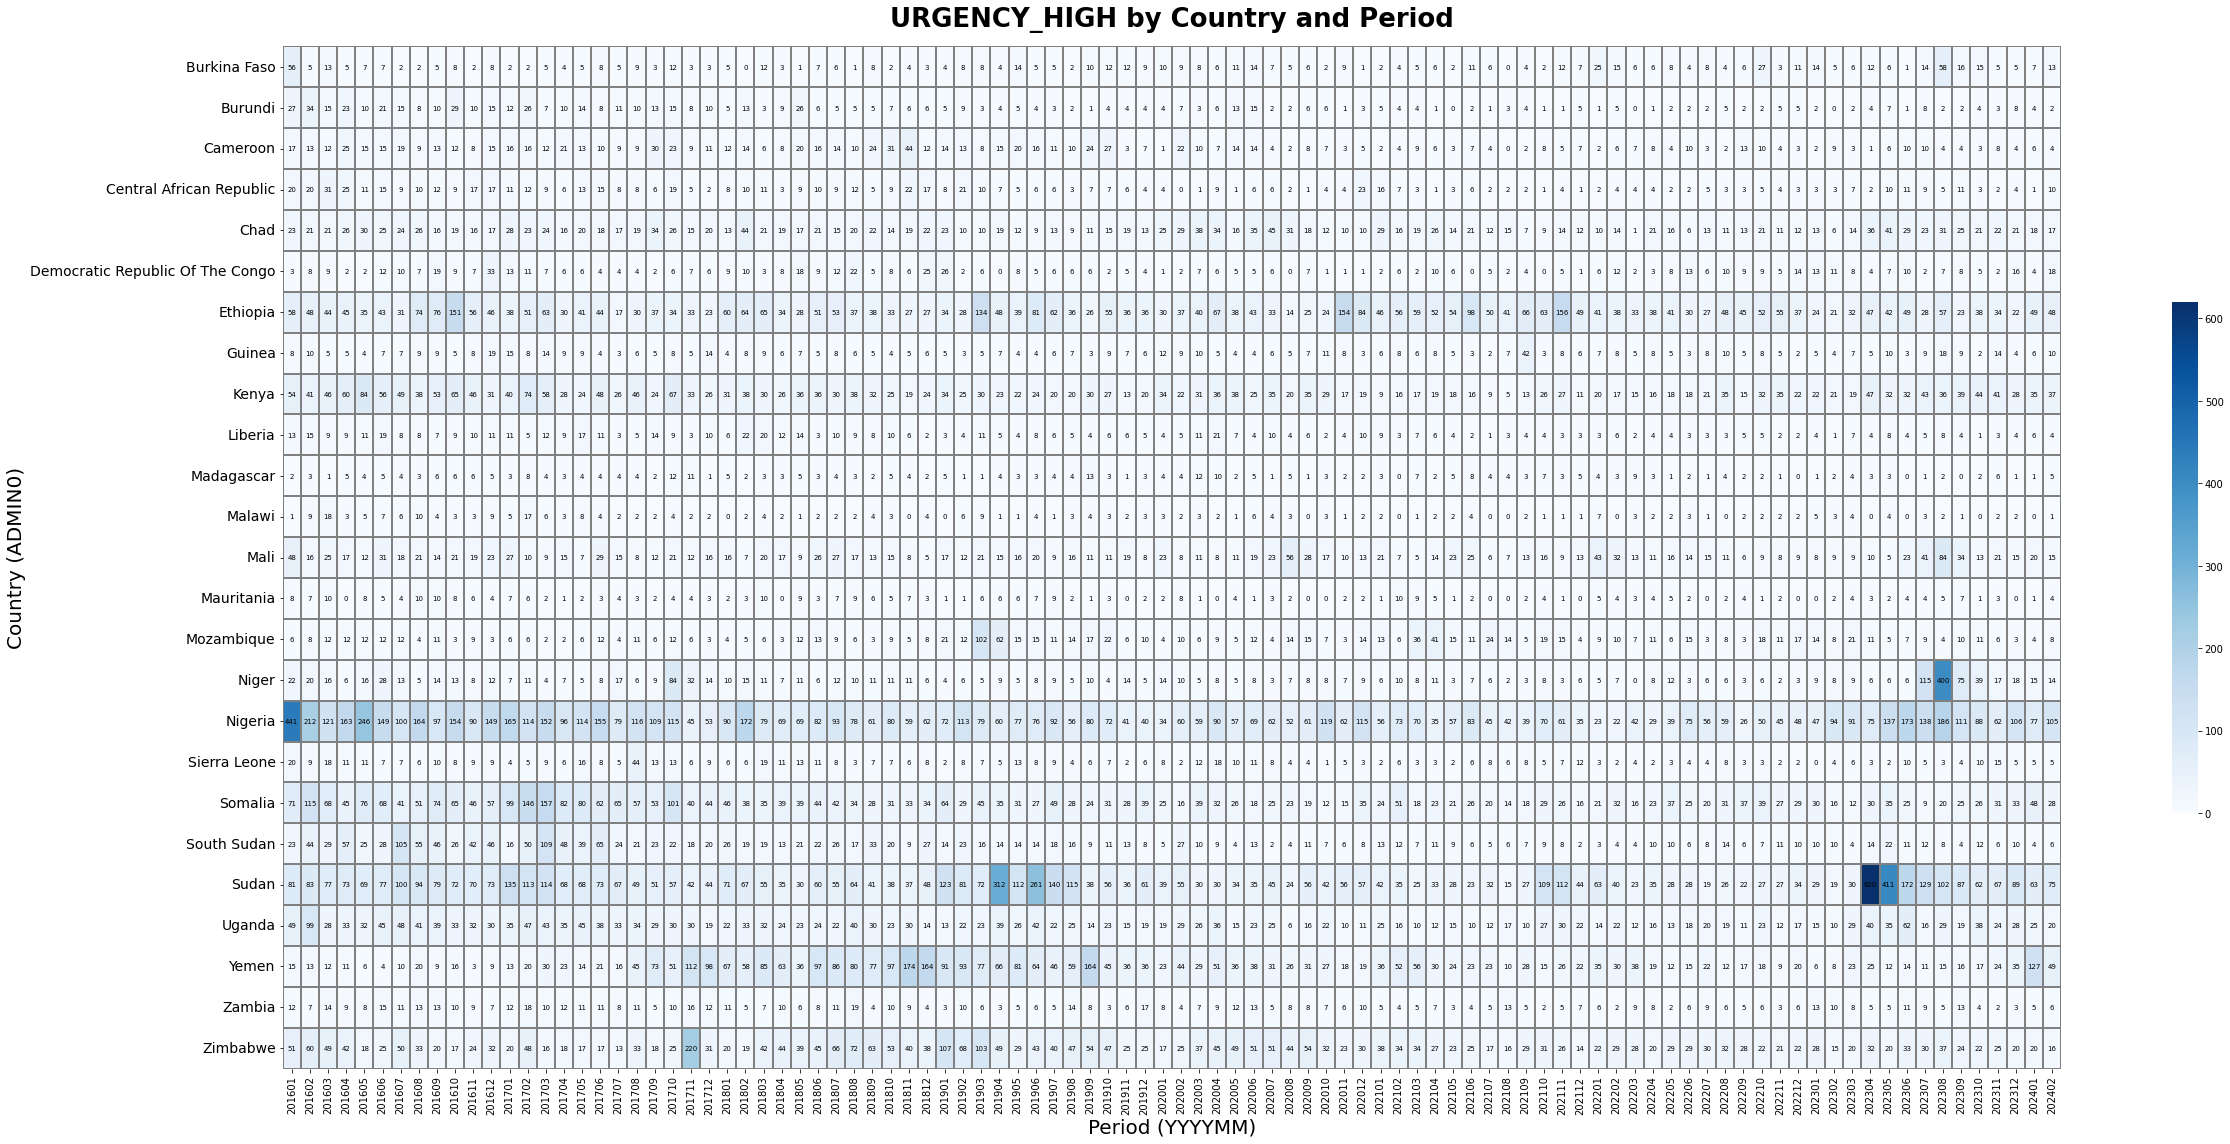
\includegraphics[width=\textwidth]{urgency_high.png}
    \caption{\textbf{S16: High urgency event frequency.} Strong spatial and temporal heterogeneity, highlighting acute crisis periods.}
\end{figure}

\begin{figure}[H]
    \centering
    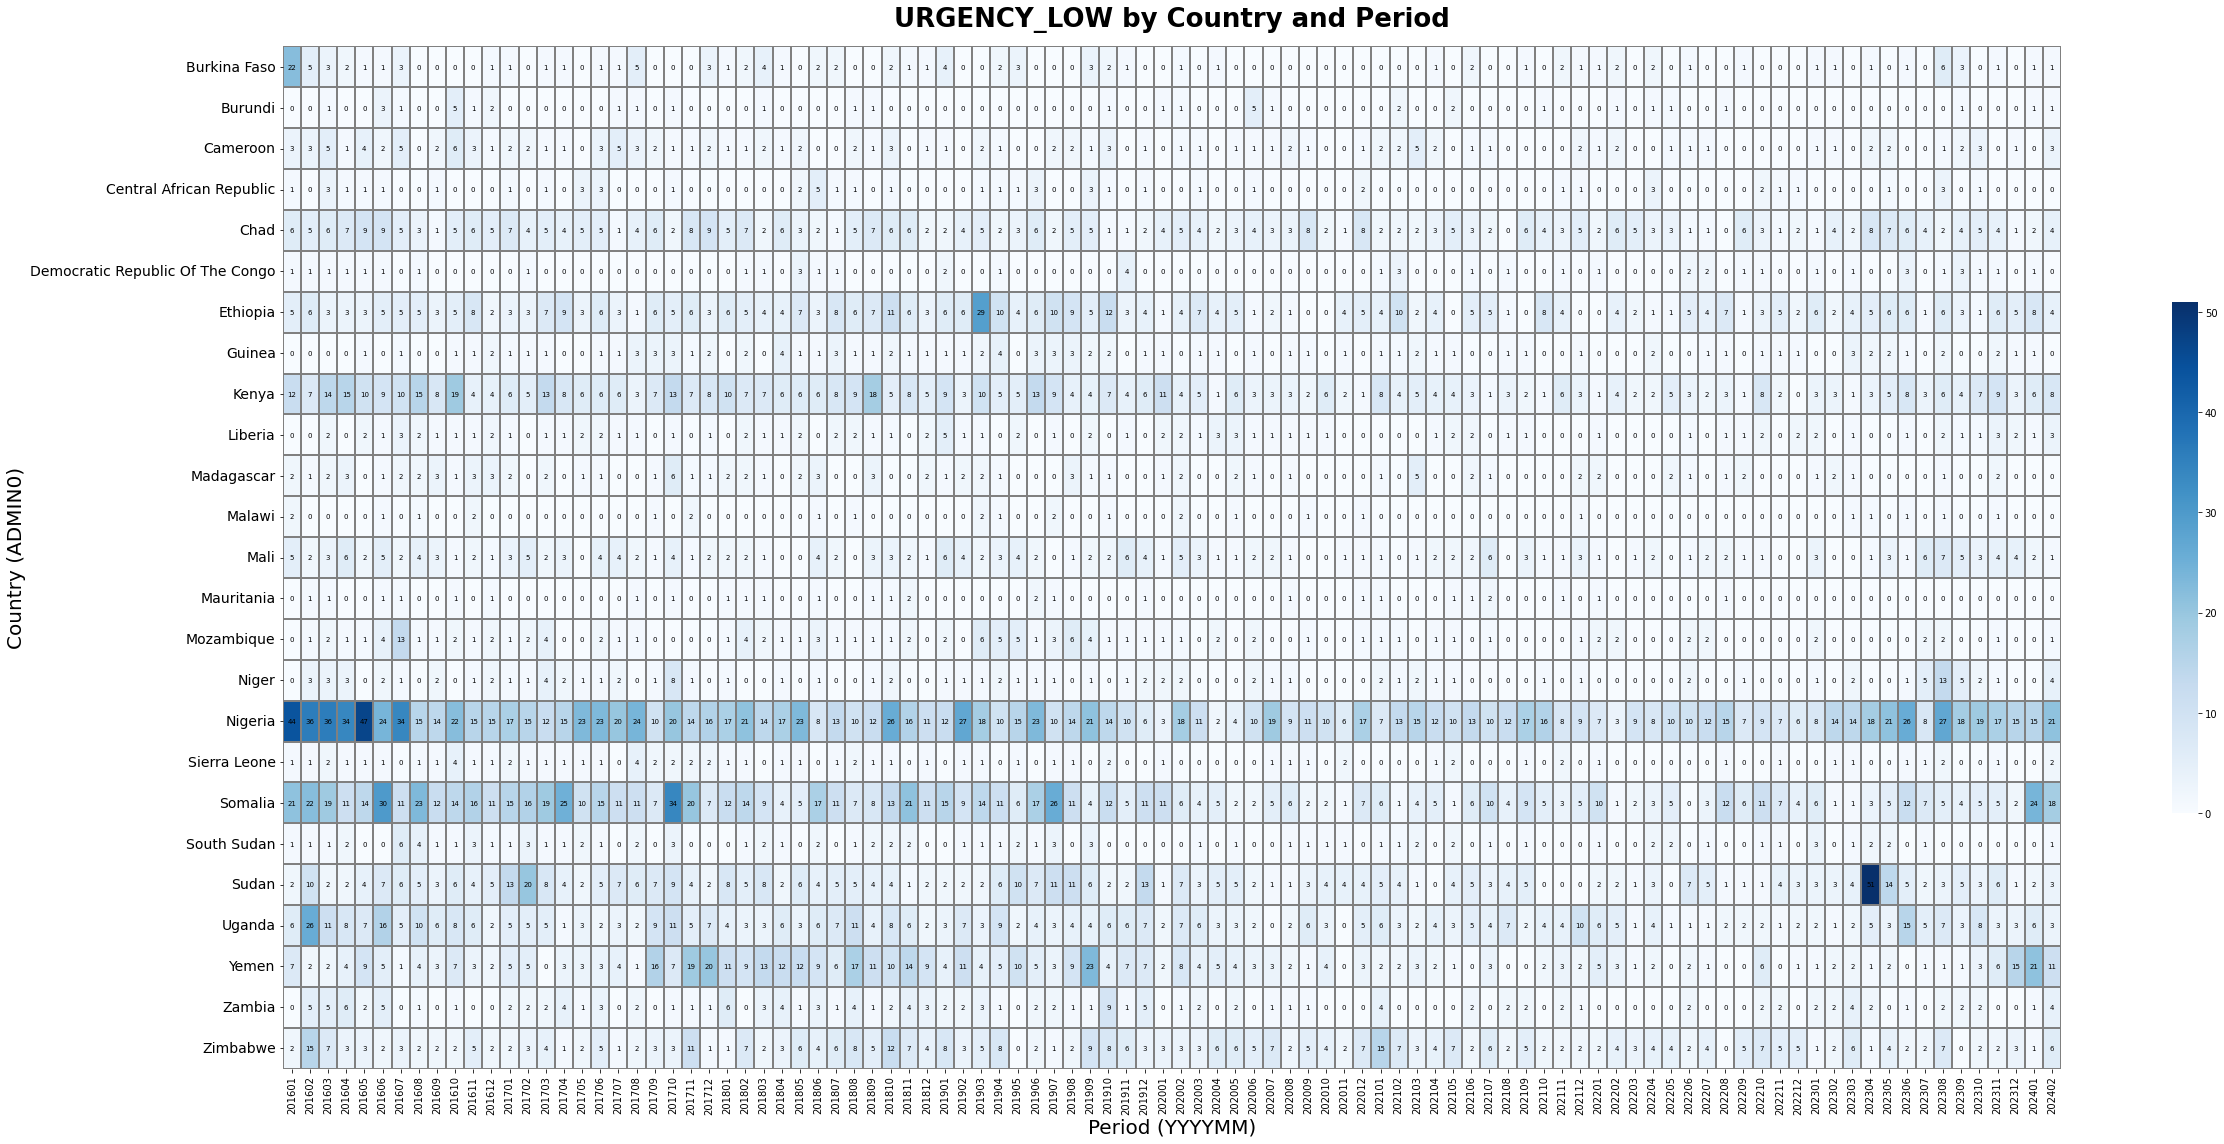
\includegraphics[width=\textwidth]{urgency_low.png}
    \caption{\textbf{S17: Low urgency event frequency.} More uniform distribution, contrasting with high-urgency signals.}
\end{figure}


% ---- GKG Heatmaps Appendix ----
\section{Supplementary Figures: GDELT GKG Diagnostics}

This section presents diagnostic heatmaps for key features extracted from GDELT GKG data (2017–2024), across ADMIN2 regions and monthly periods.

\begin{figure}[H]
    \centering
    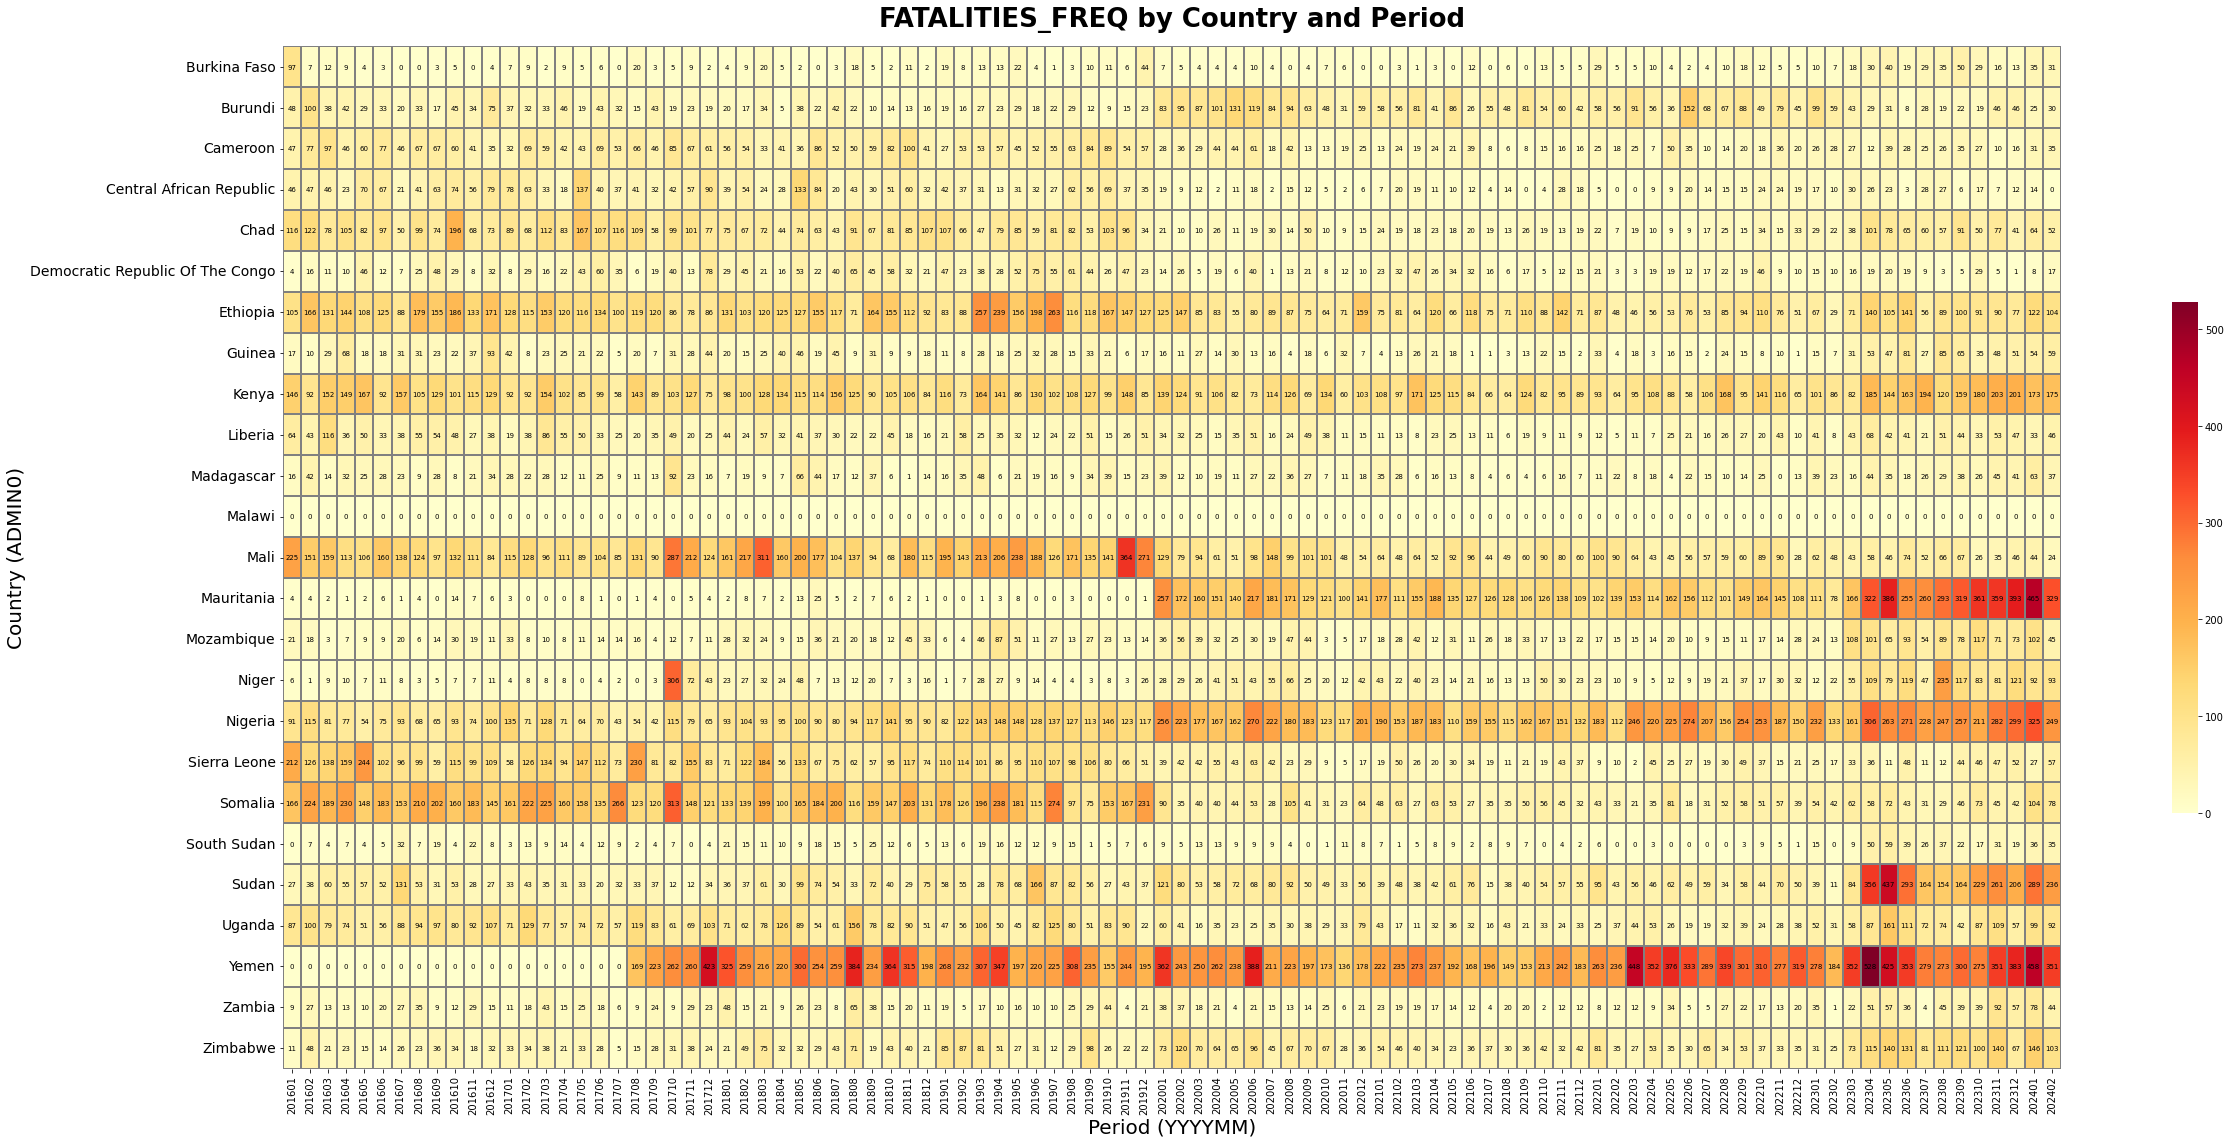
\includegraphics[width=\textwidth]{fatalities_gkg_freq.png}
    \caption{\textbf{S18:} Heatmap of fatalities frequency (GKG). Captures episodic and regional spikes in reported deaths.}
\end{figure}

\begin{figure}[H]
    \centering
    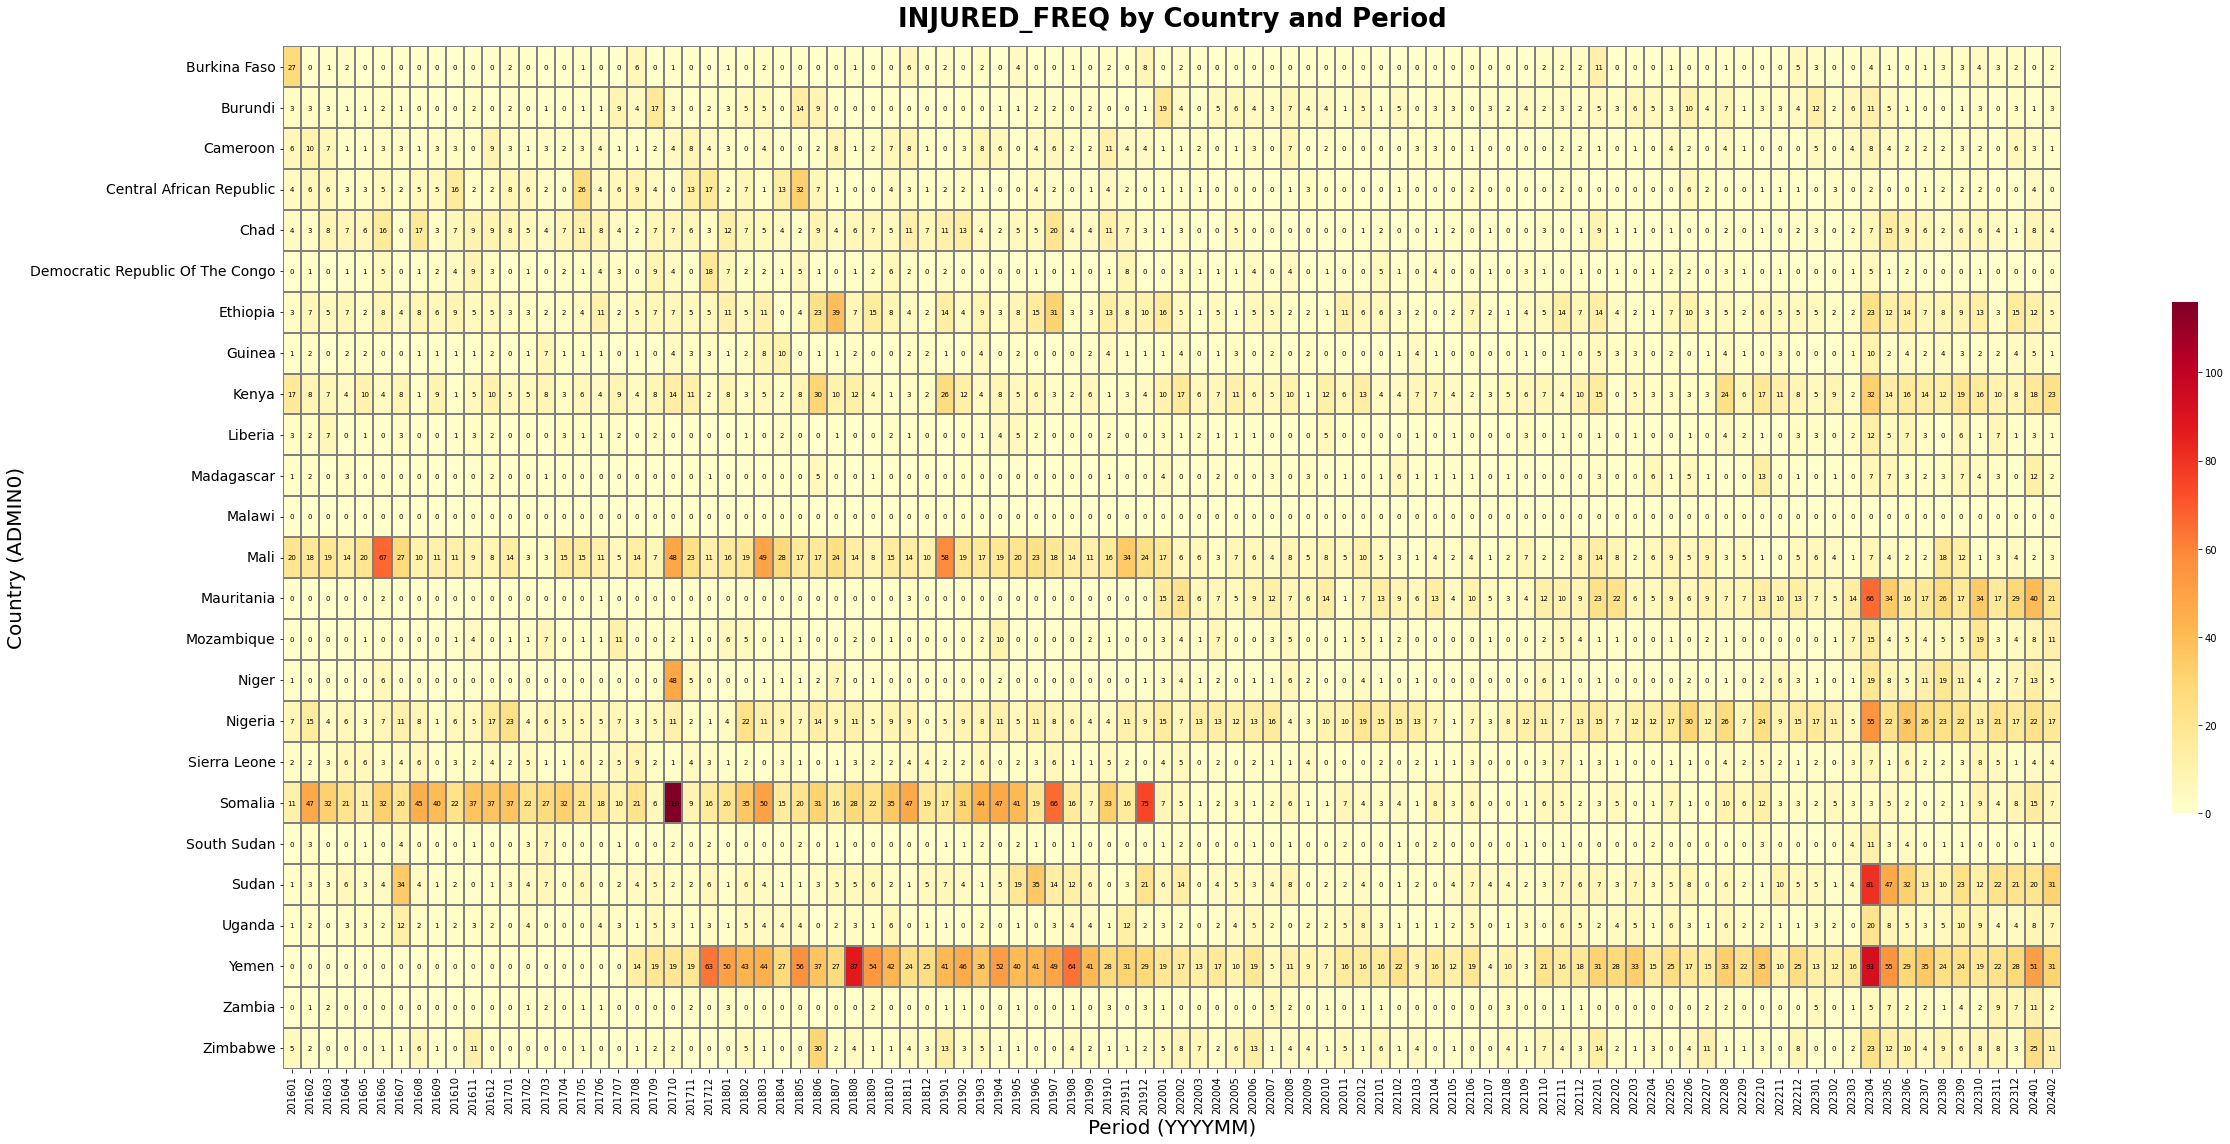
\includegraphics[width=\textwidth]{injured_gkg_freq.png}
    \caption{\textbf{S19:} Heatmap of injured frequency (GKG). Temporal clusters indicate major violent events.}
\end{figure}

\begin{figure}[H]
    \centering
    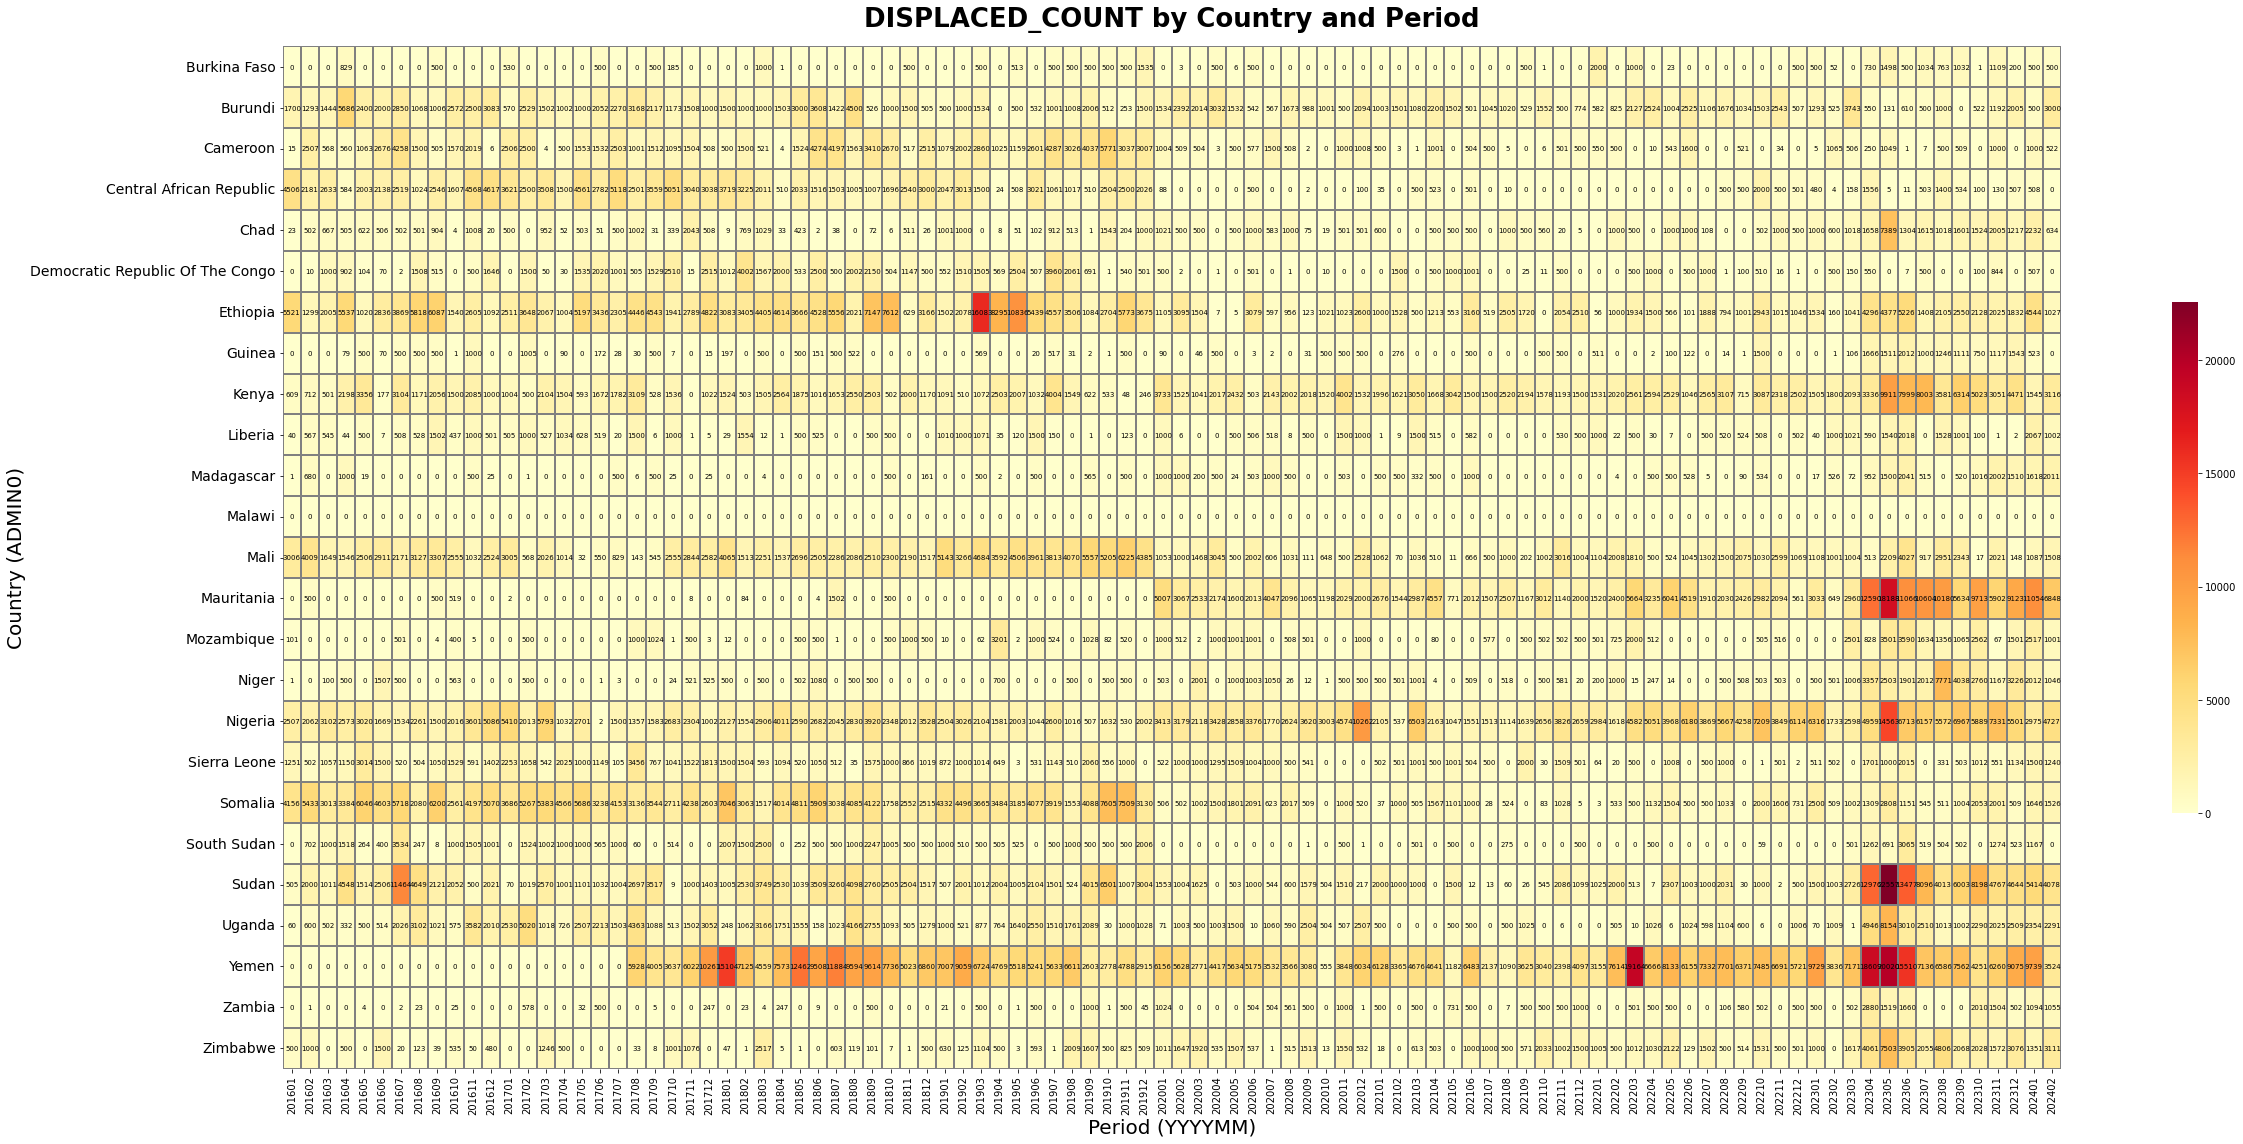
\includegraphics[width=\textwidth]{displaced_gkg_count.png}
    \caption{\textbf{S20:} Heatmap of displacement event counts (GKG). Highlights periods of increased population movement.}
\end{figure}

\begin{figure}[H]
    \centering
    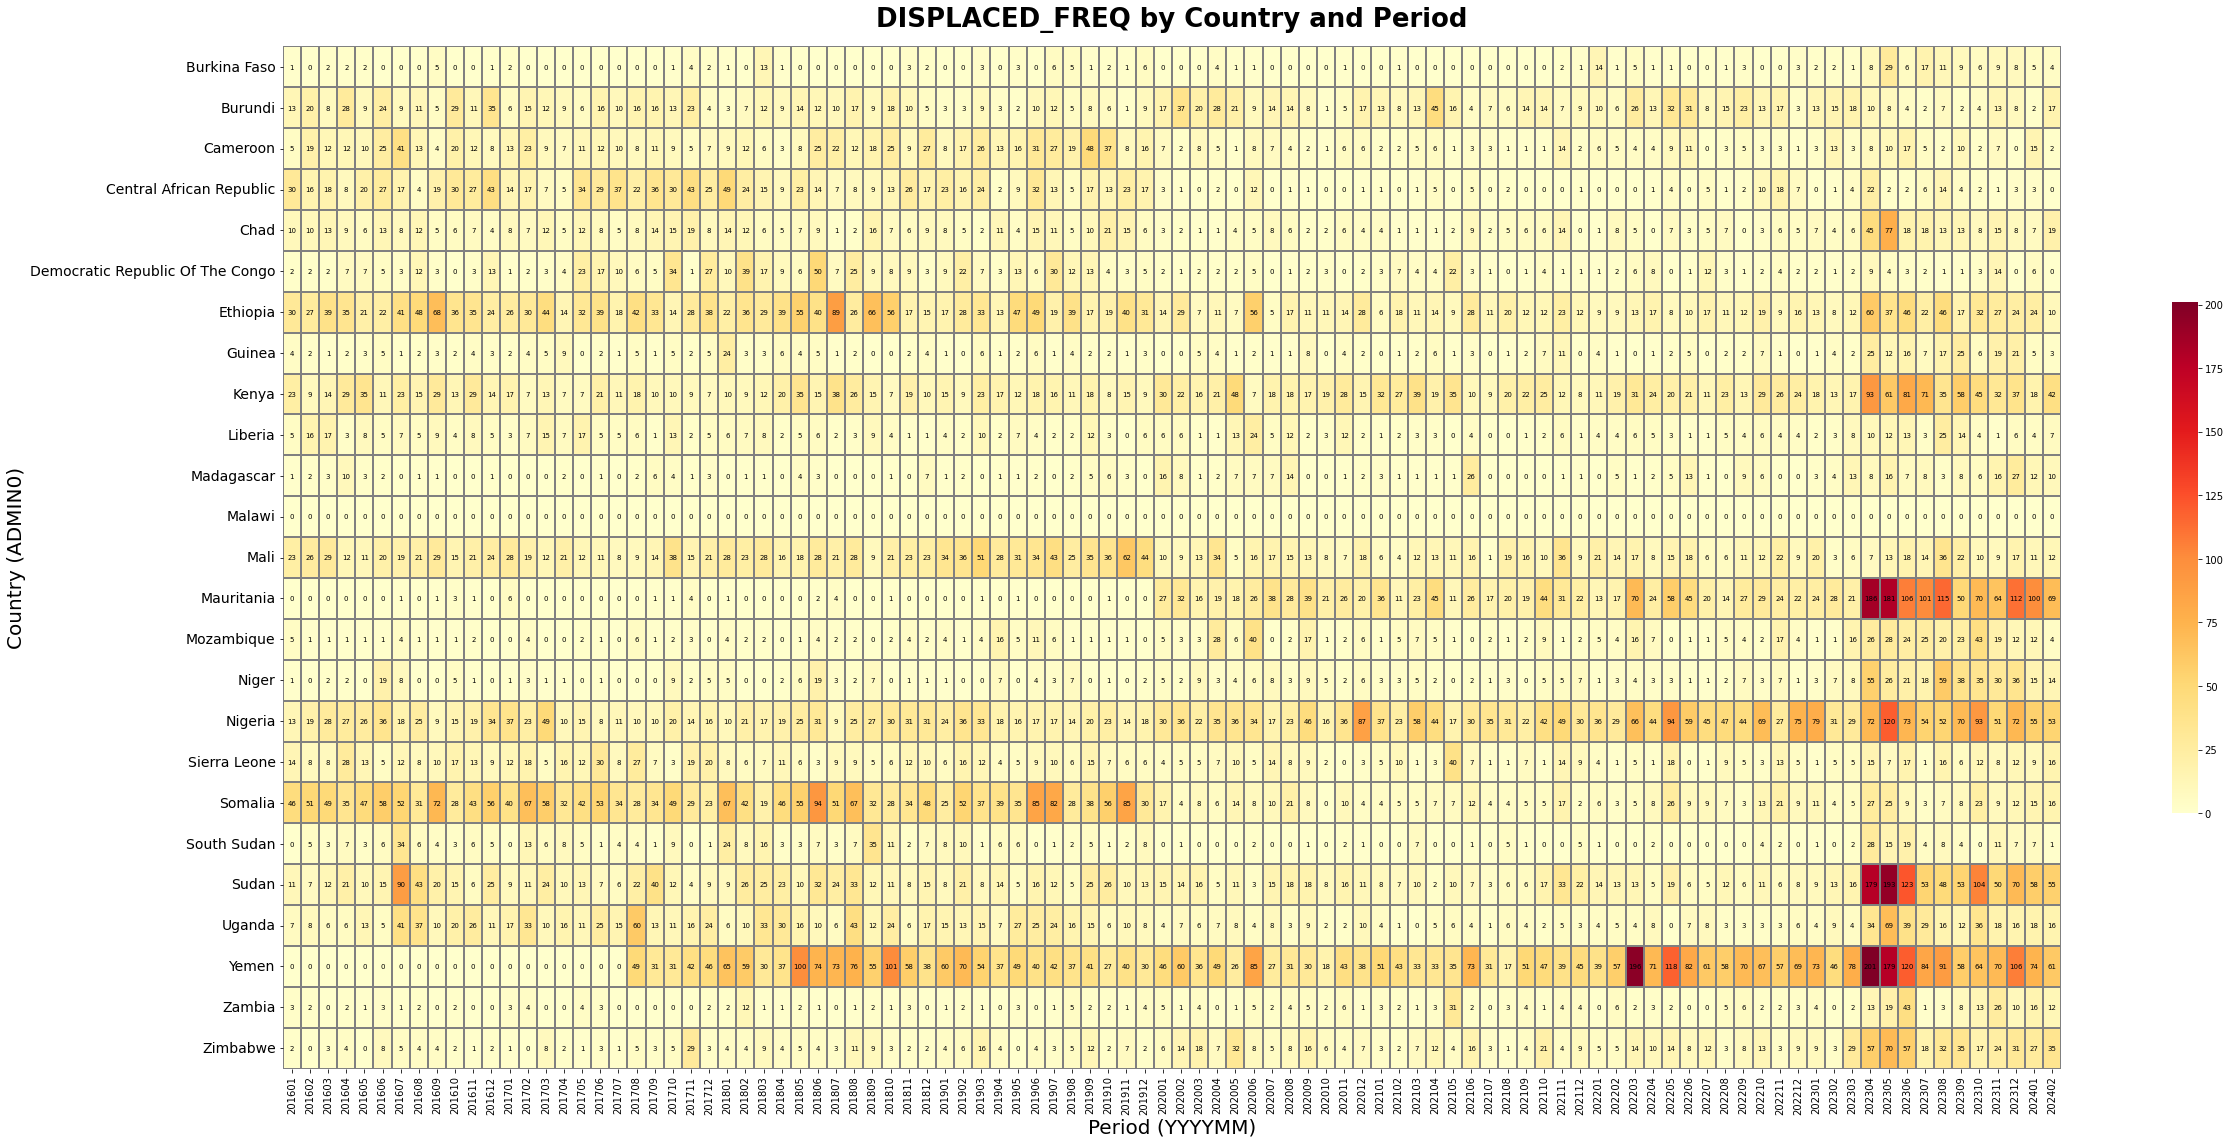
\includegraphics[width=\textwidth]{displaced_gkg_freq.png}
    \caption{\textbf{S21:} Heatmap of displaced persons frequency (GKG). Localized peaks track major displacement episodes.}
\end{figure}

\begin{figure}[H]
    \centering
    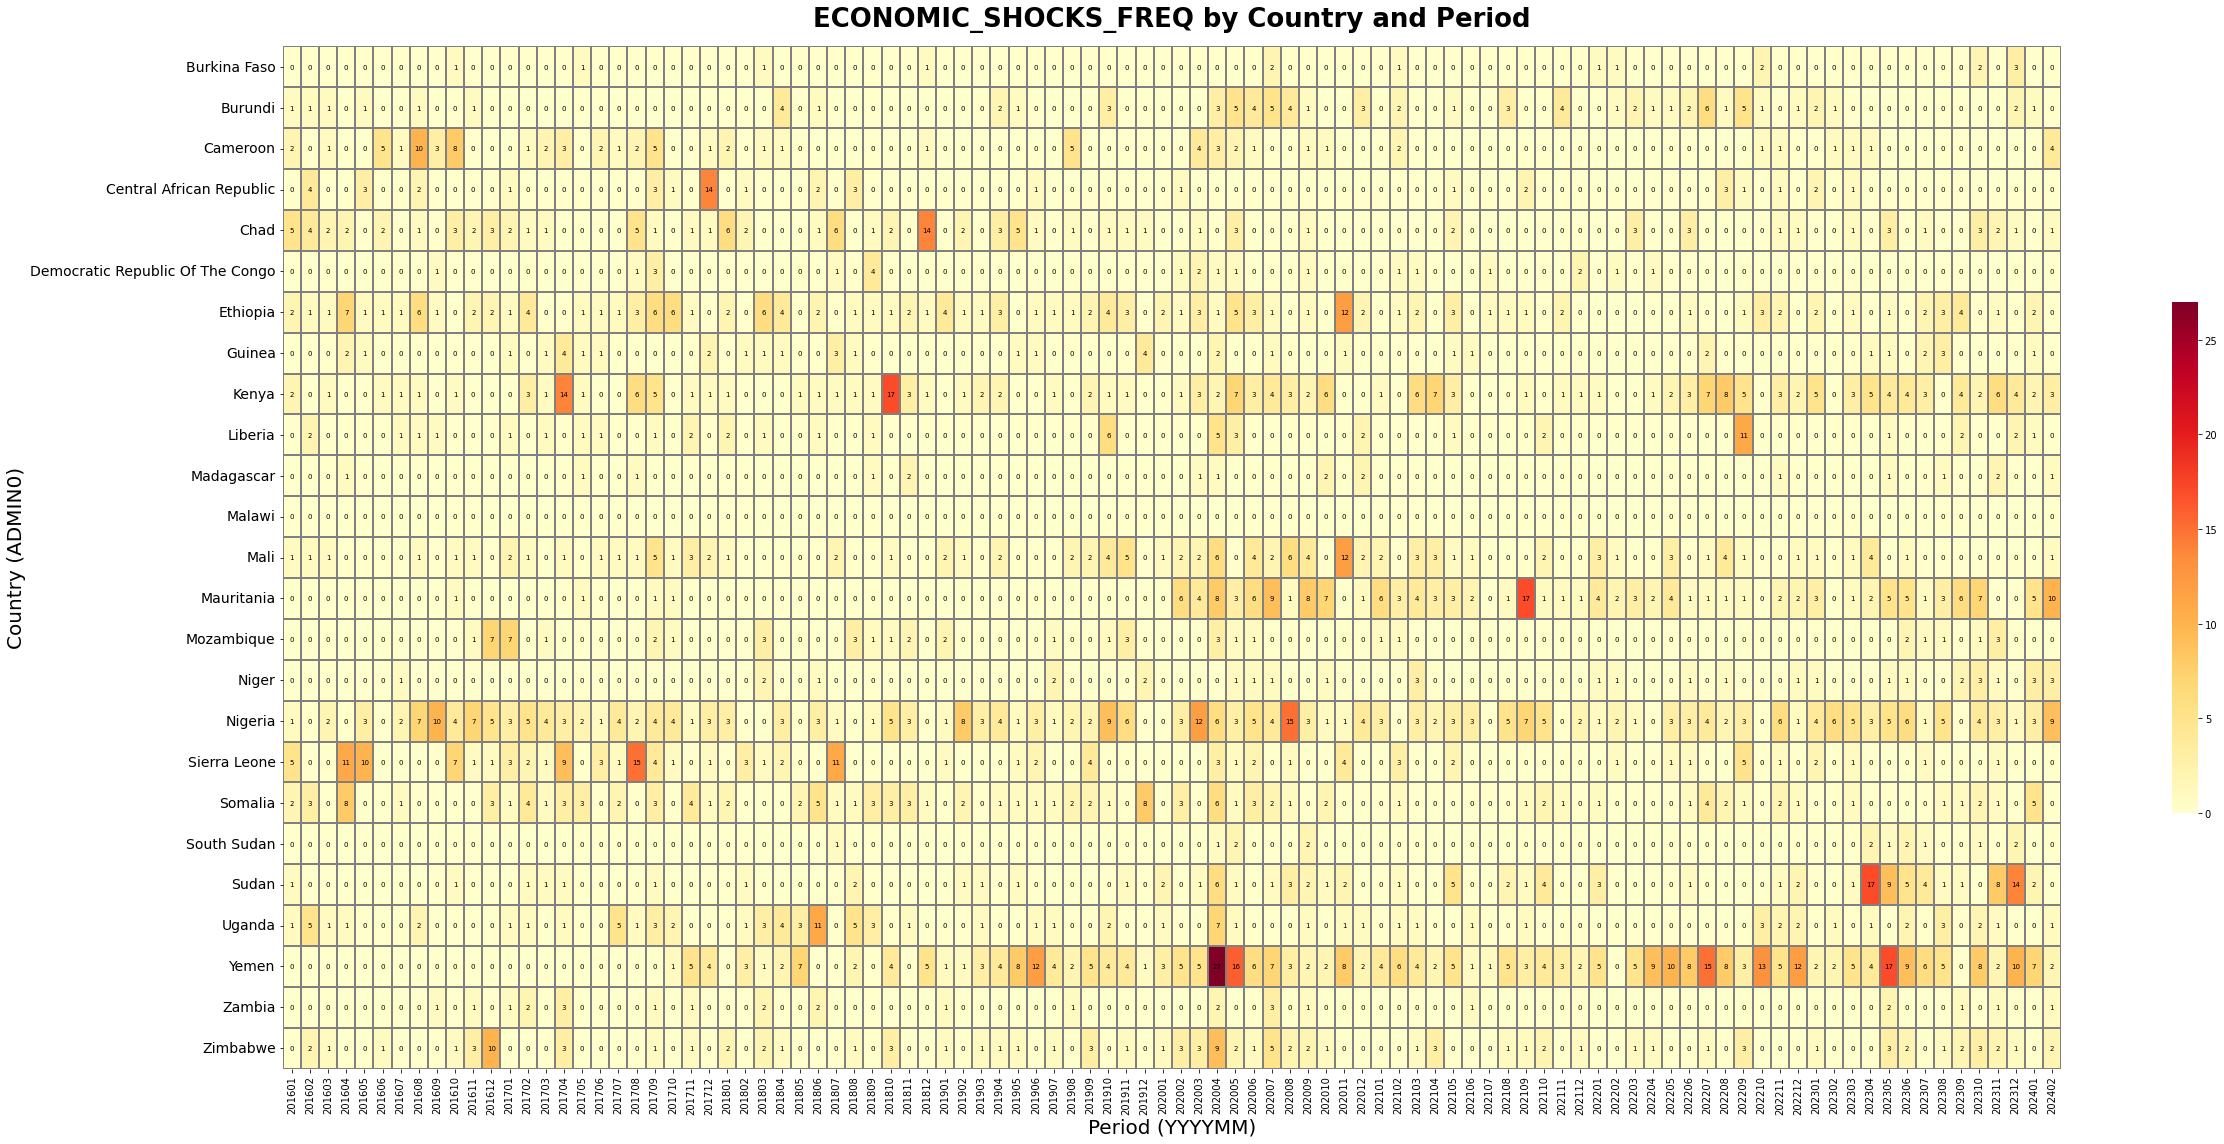
\includegraphics[width=\textwidth]{econ_schock_gkg.png}
    \caption{\textbf{S22:} Heatmap of economic shock mentions (GKG). Highlights acute periods of reported economic instability.}
\end{figure}

\begin{figure}[H]
    \centering
    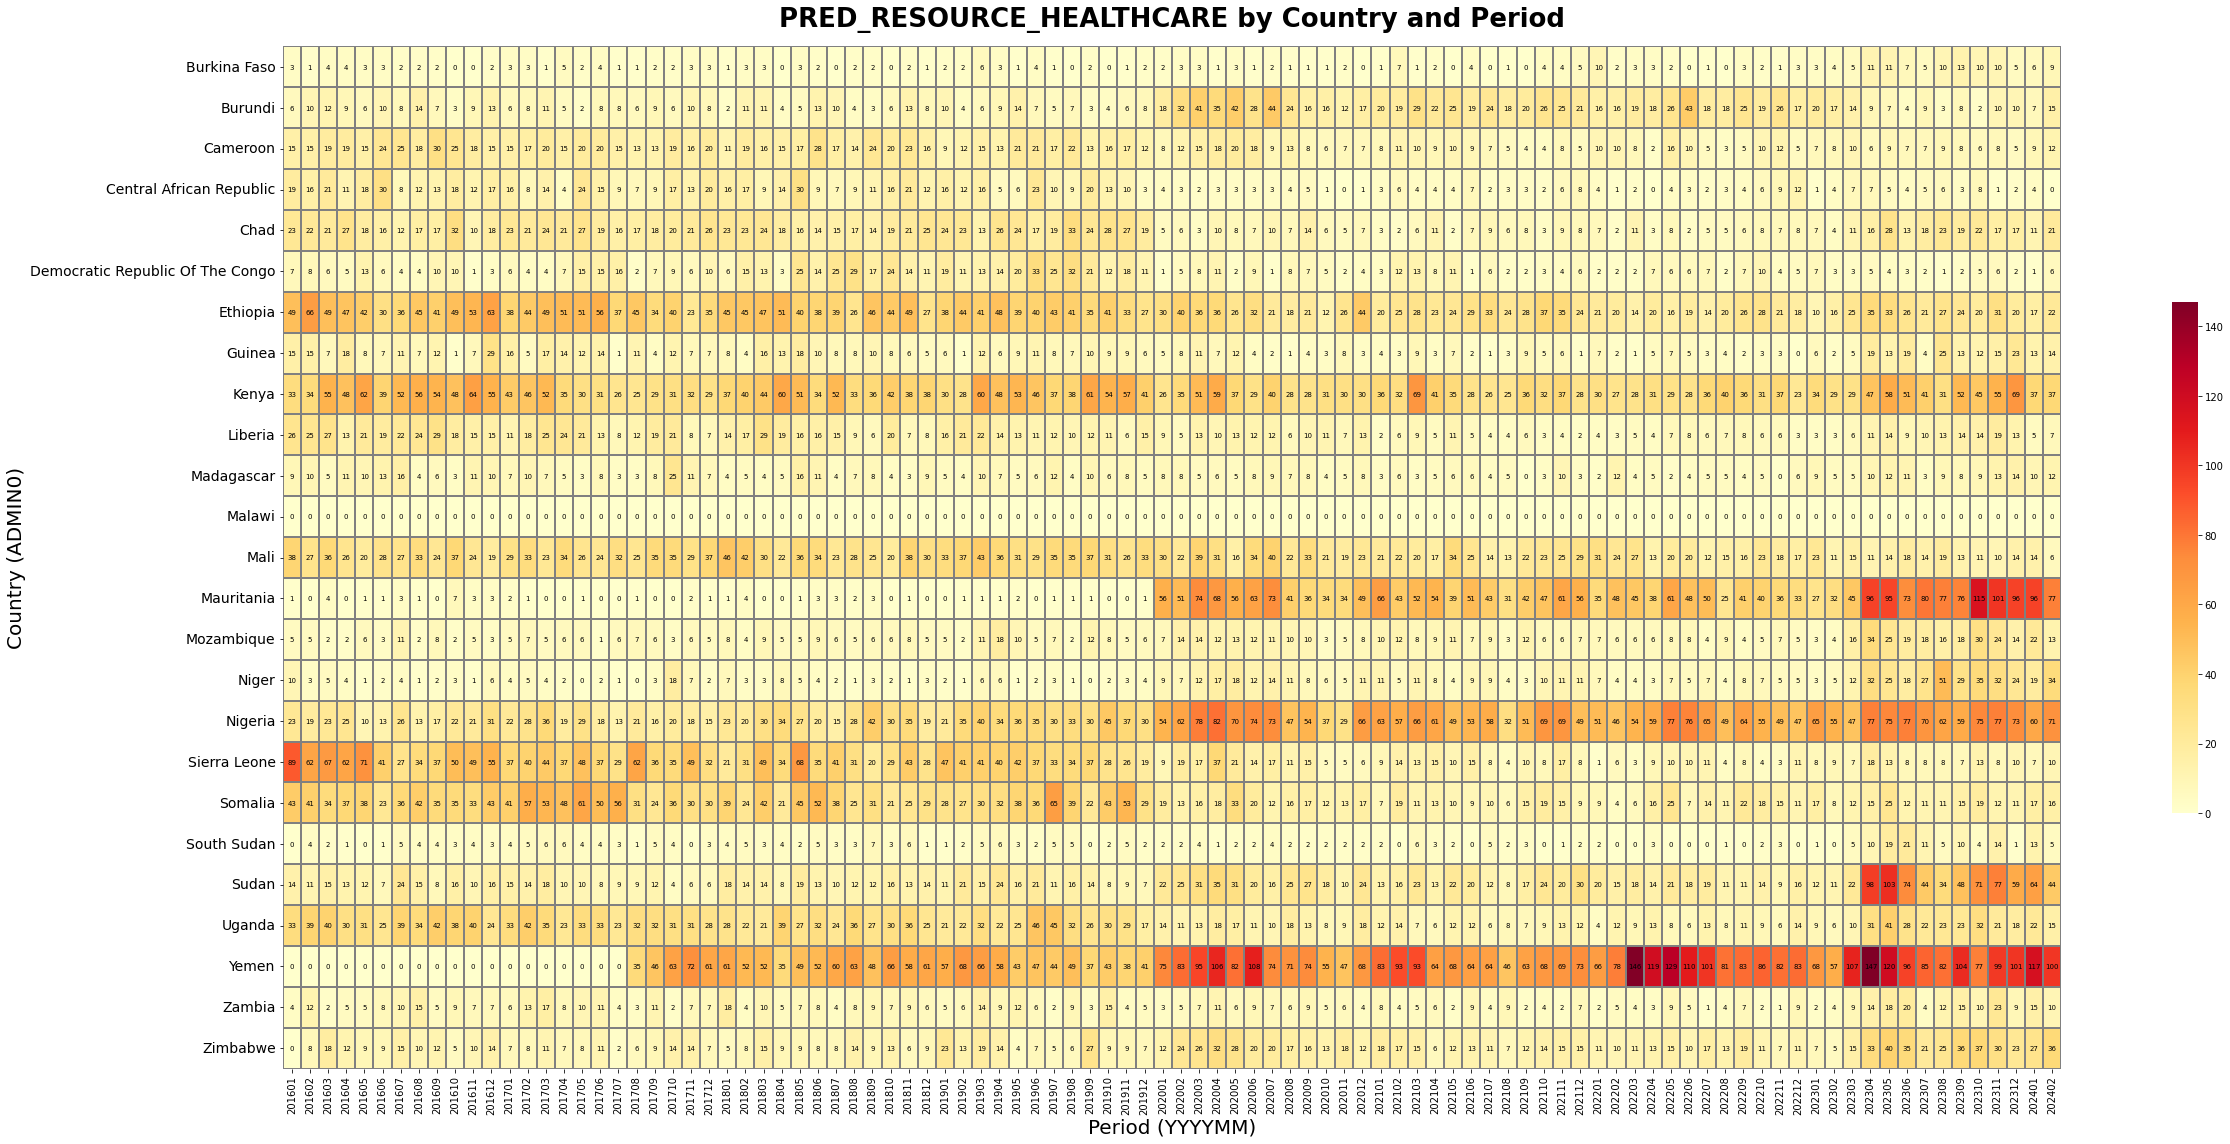
\includegraphics[width=\textwidth]{pred_resource_cash_gkg.png}
    \caption{\textbf{S23:} Heatmap of predicted need for cash assistance (GKG). Regional clustering of high demand is evident.}
\end{figure}

\begin{figure}[H]
    \centering
    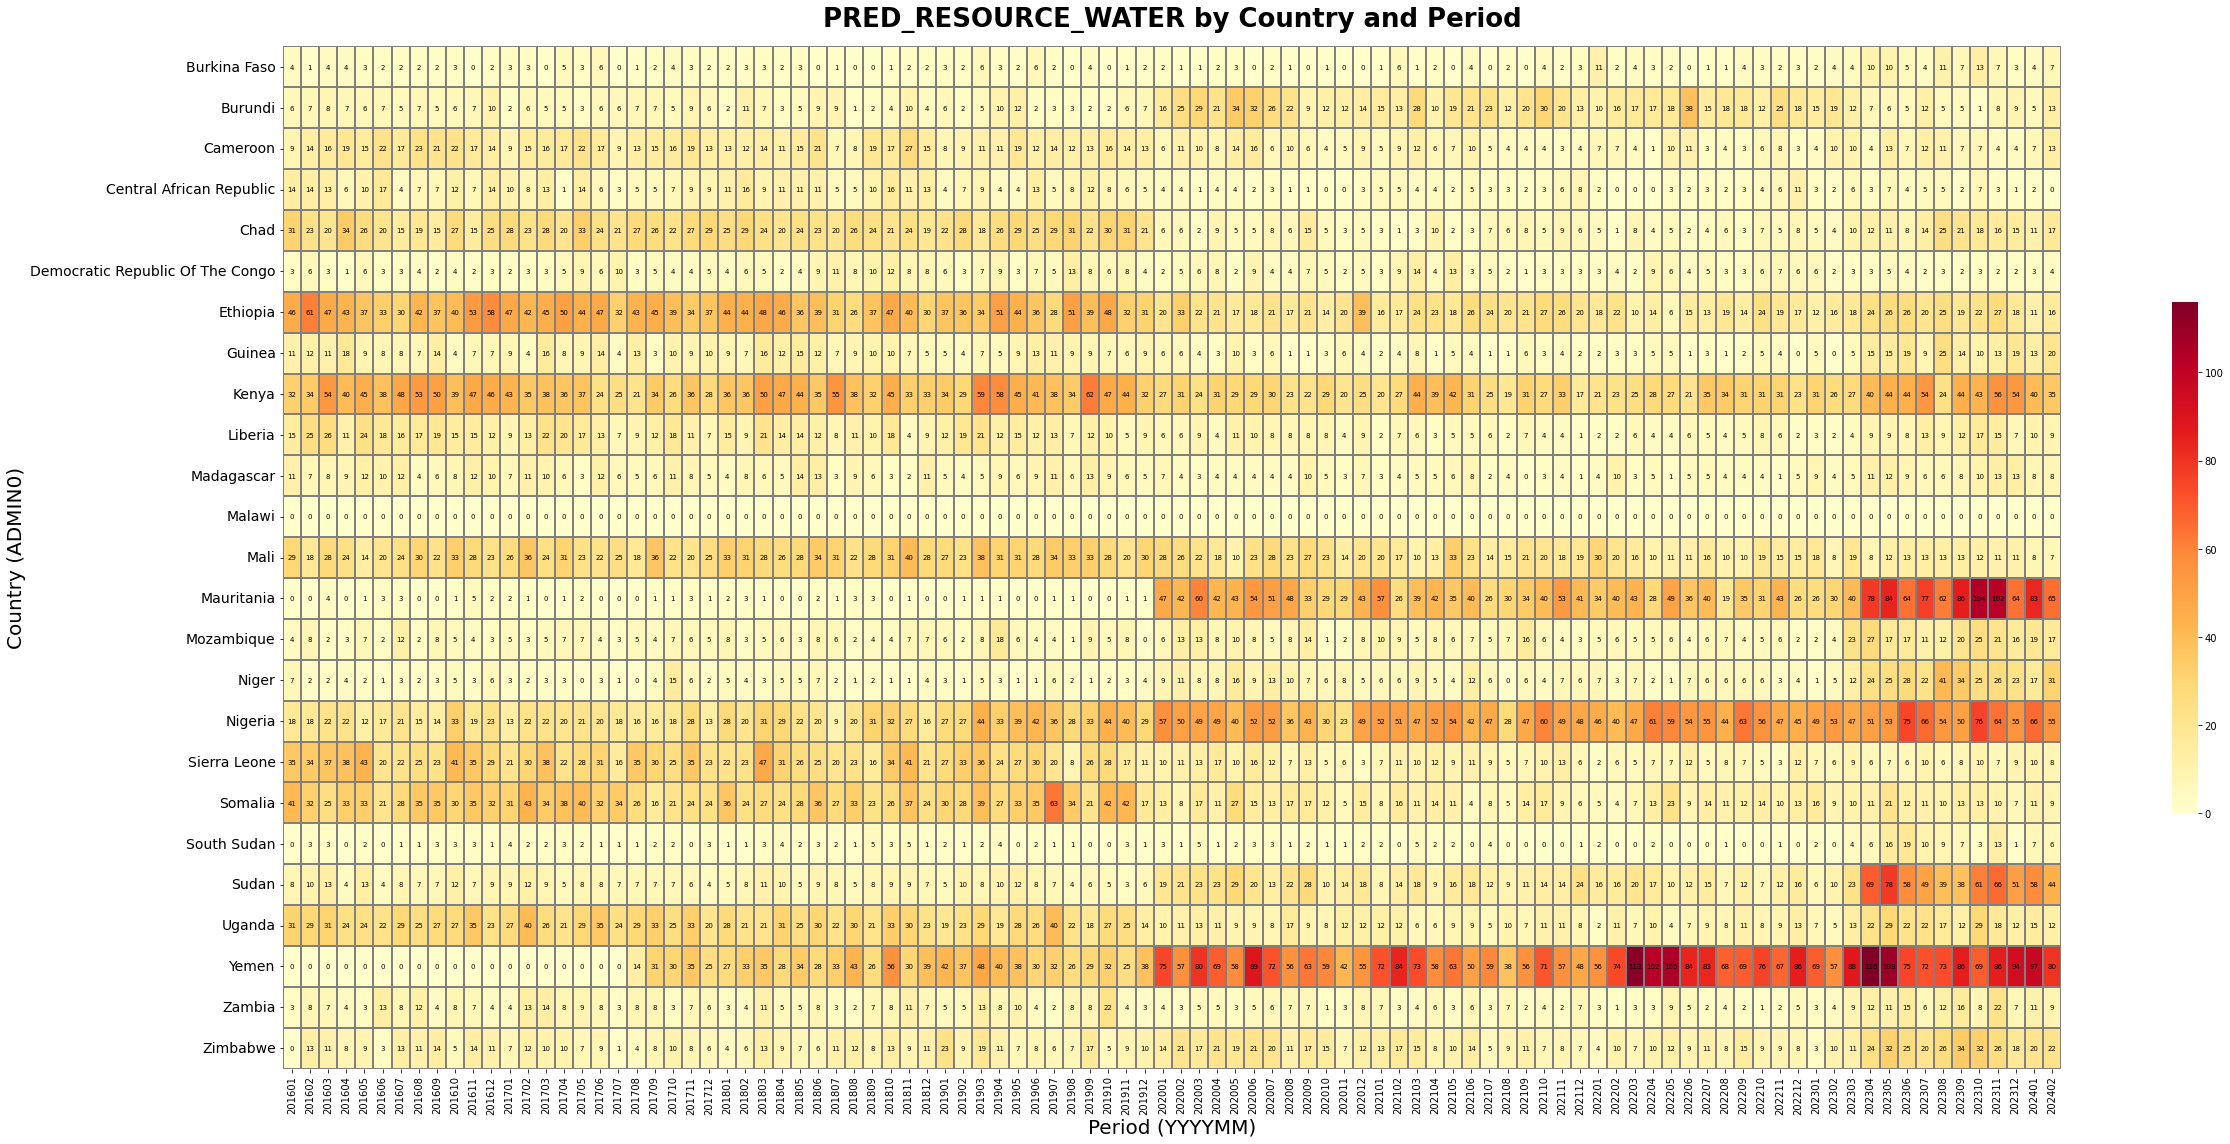
\includegraphics[width=\textwidth]{pred_resource_water_gkg.png}
    \caption{\textbf{S24:} Heatmap of predicted need for water aid (GKG). Scattered peaks indicate emerging crises.}
\end{figure}

\begin{figure}[H]
    \centering
    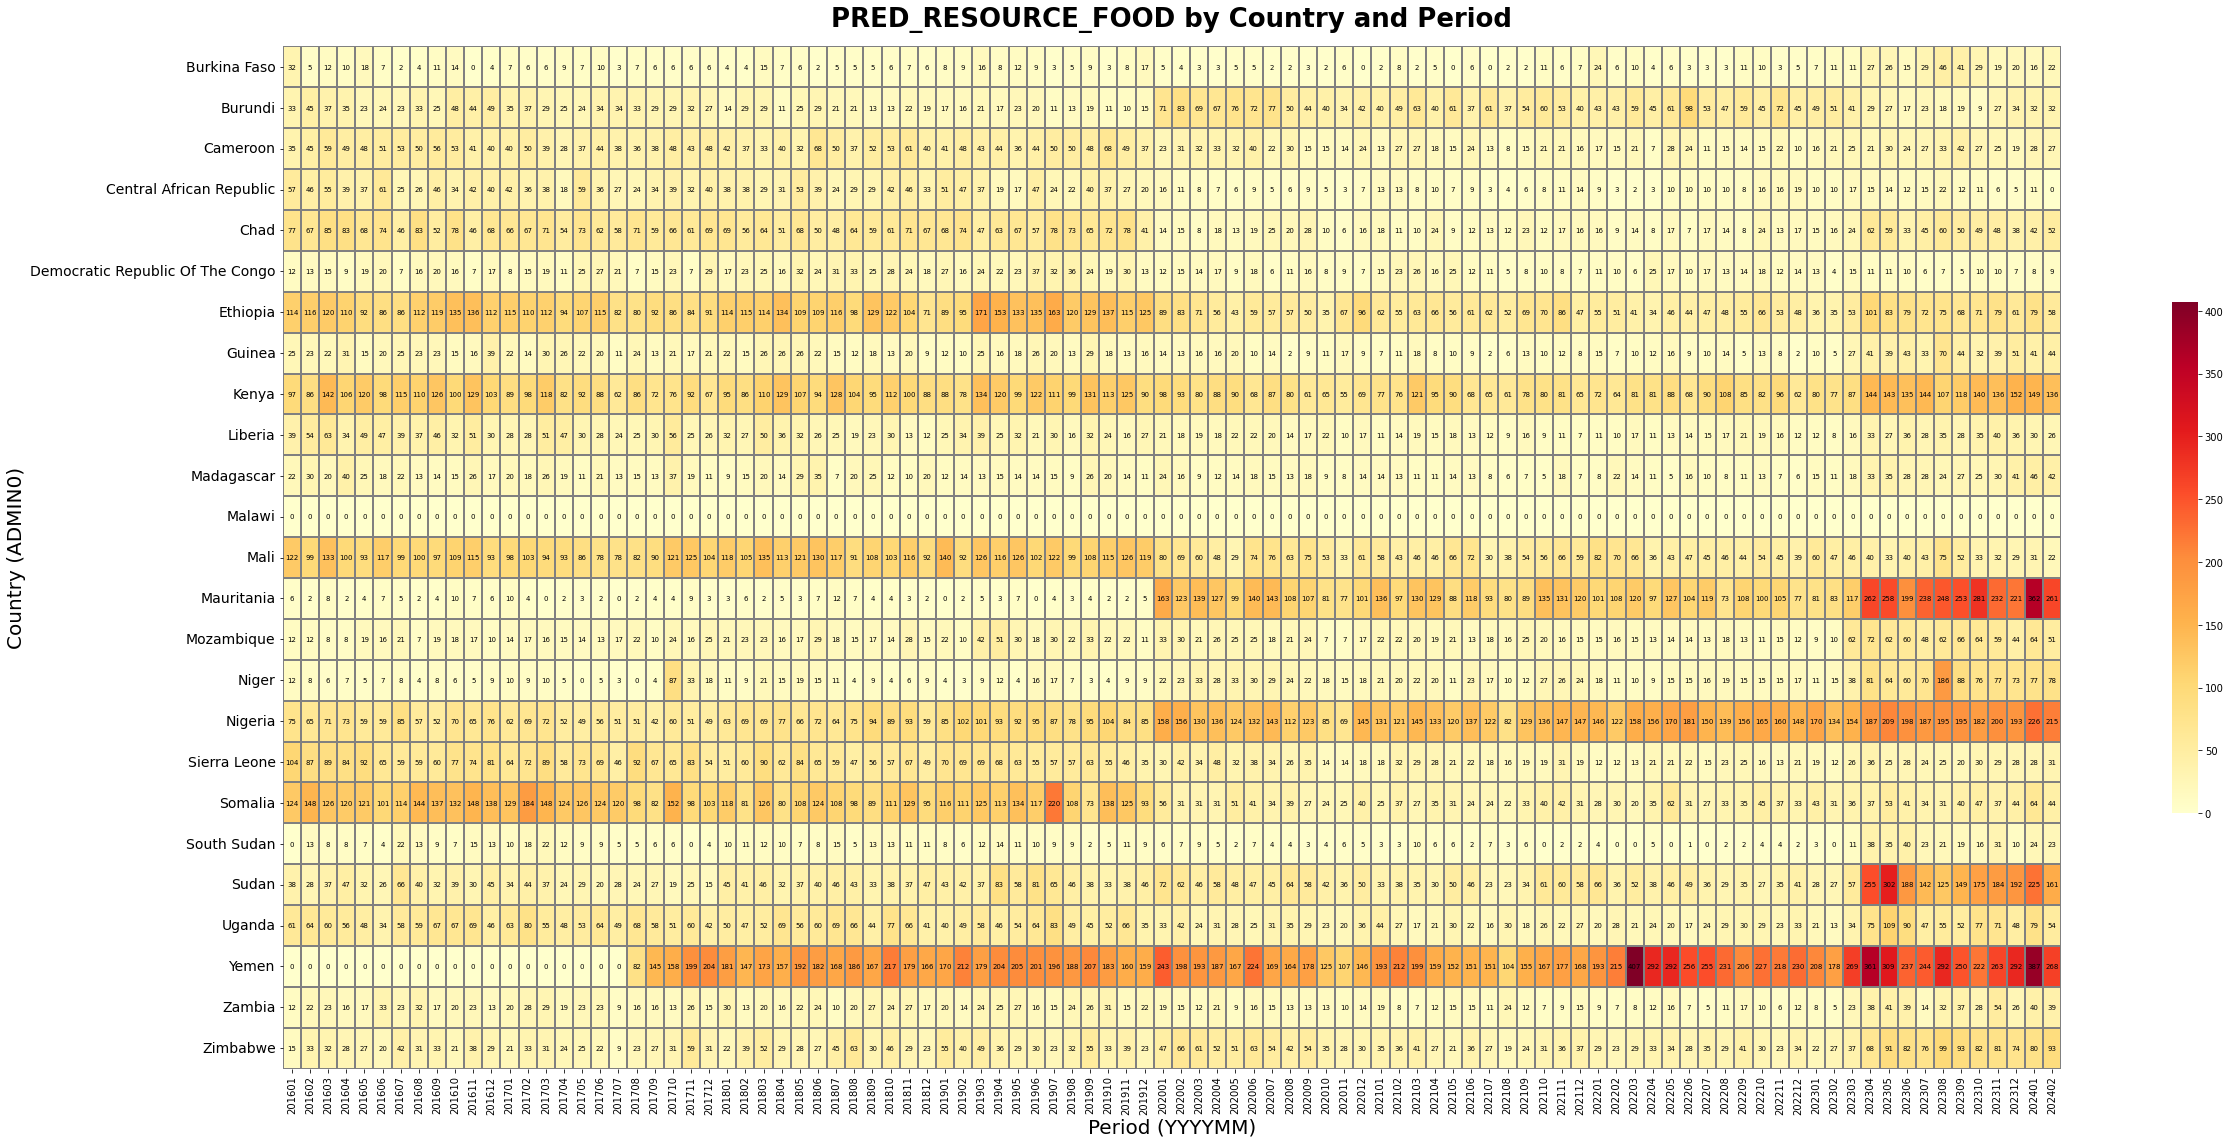
\includegraphics[width=\textwidth]{pred_resources_food_gkg.png}
    \caption{\textbf{S25:} Heatmap of predicted need for food aid (GKG). Strongest signals align with well-documented food emergencies.}
\end{figure}

\begin{figure}[H]
    \centering
    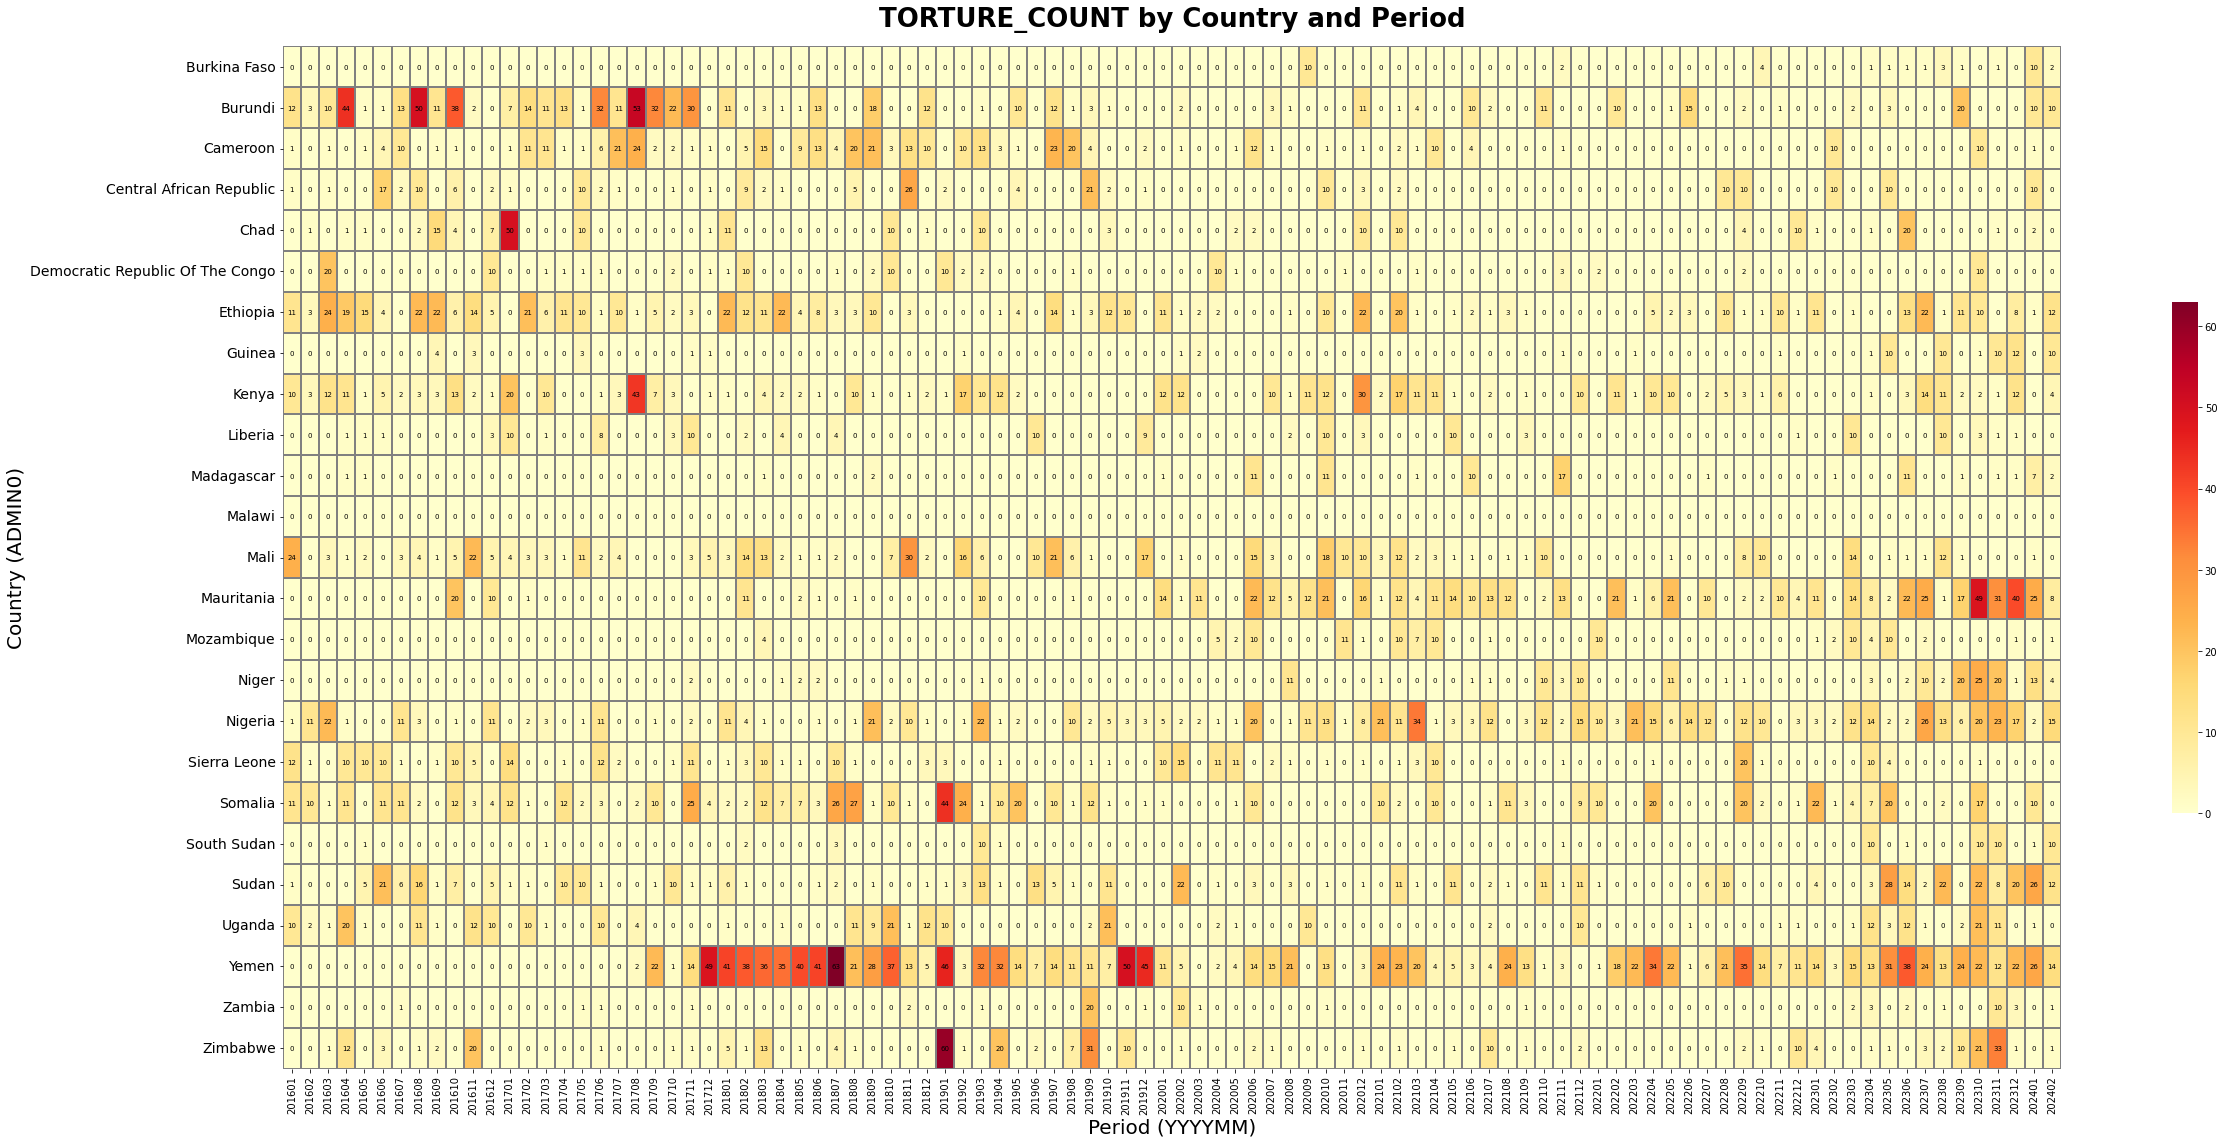
\includegraphics[width=\textwidth]{torture_count_gkg.png}
    \caption{\textbf{S26:} Heatmap of torture event counts (GKG). Isolated but highly localized reports are visible.}
\end{figure}

\begin{figure}[H]
    \centering
    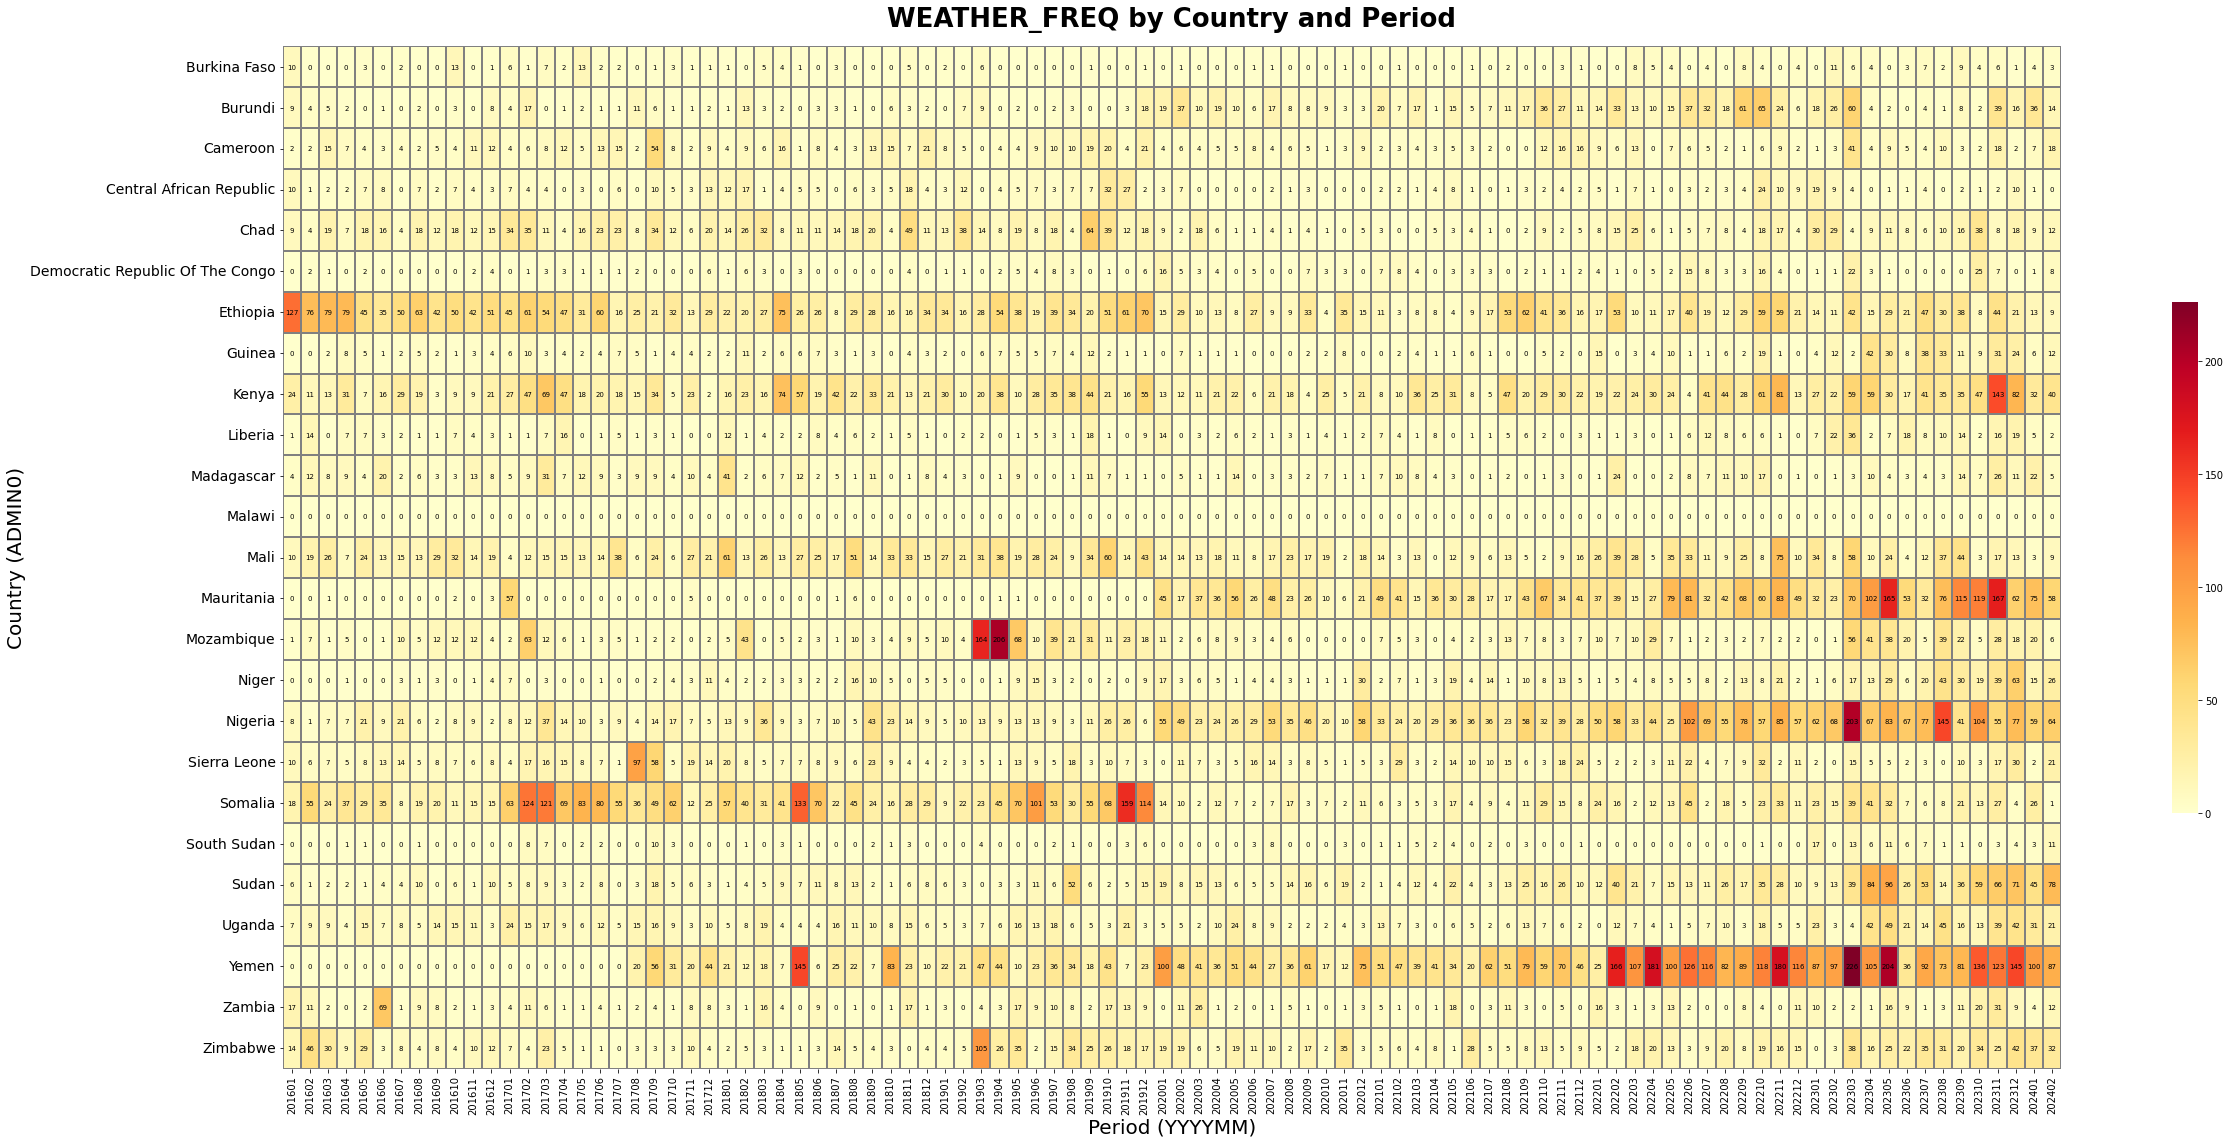
\includegraphics[width=\textwidth]{weather_freq_gkg.png}
    \caption{\textbf{S27:} Heatmap of weather event frequency (GKG). Peaks correspond to periods of climate-related reporting.}
\end{figure}

\end{document}
